\documentclass[12pt]{article}
\usepackage{graphicx}
\usepackage{booktabs}
\usepackage{geometry}
\usepackage{amsmath}
\geometry{margin=1in}
\title{Quantitative Analysis of Seasonal Decomposition and Monthly Returns in NEPSE Subindices}
\author{Your Research Team}
\date{July 29, 2025}
\begin{document}
\maketitle
\begin{abstract}
This report presents a comprehensive quantitative analysis of the monthly return seasonality and trend decomposition for major NEPSE subindices. Using time series decomposition, we extract and evaluate the trend, seasonal, and residual components of monthly returns for each sector. The findings reveal robust and statistically significant seasonal patterns, with actionable insights for tactical asset allocation and risk management in the Nepalese equity market.
\end{abstract}
\section{Introduction}
The Nepal Stock Exchange (NEPSE) comprises various sectoral indices, each reflecting the performance of a specific segment of the Nepalese capital market. Understanding the seasonal and cyclical behavior of these indices is crucial for investors seeking to optimize returns and manage risk. This study applies additive seasonal decomposition to monthly returns of NEPSE subindices, aiming to uncover persistent patterns and inform investment strategy.
\section{Methodology}
\subsection{Data}
We use historical close prices for each NEPSE subindex, resampled to monthly frequency. The analysis covers all available data up to July 2025.
\subsection{Return Calculation}
Monthly returns are calculated as:
\[
R_{m} = \frac{P_{m, \text{last}} - P_{m, \text{first}}}{P_{m, \text{first}}} \times 100
\]
where $P_{m, \text{last}}$ and $P_{m, \text{first}}$ are the last and first close prices of month $m$.
\subsection{Decomposition}
We apply additive seasonal decomposition with a 12-month period to the monthly return series, extracting:
\begin{itemize}
    \item \textbf{Trend:} Long-term movement in returns.
    \item \textbf{Seasonal:} Repeating annual pattern.
    \item \textbf{Residual:} Unexplained, random component.
\end{itemize}
\subsection{Statistical Metrics}
For each sector, we compute:
\begin{itemize}
    \item Mean, median, and standard deviation of monthly returns.
    \item Month-wise average returns and seasonality.
    \item Frequency of positive/negative returns per month.
    \item Maximum drawdown and annualized volatility.
\end{itemize}
\section{Aggregate Market Seasonality}
Across all subindices, July consistently delivers the highest average returns, while August and September are typically the weakest months. Insurance and Investment sectors exhibit the highest volatility and seasonal amplitude. The annual cycle is a significant driver of monthly returns in most sectors.
\section{Sector-by-Sector Analysis}

\subsection{BANKING}
\textbf{Mean Monthly Return:} 1.16\% \\
\textbf{Median Monthly Return:} 0.54\% \\
\textbf{Standard Deviation:} 3.24\% \\
\textbf{Best Month:} Jul (9.30\%) \\
\textbf{Worst Month:} Mar (-2.16\%) \\
\textbf{Seasonal Amplitude:} 11.46\% \\
\textbf{August Return:} -1.77\% \\

\begin{figure}[h!]
    \centering
    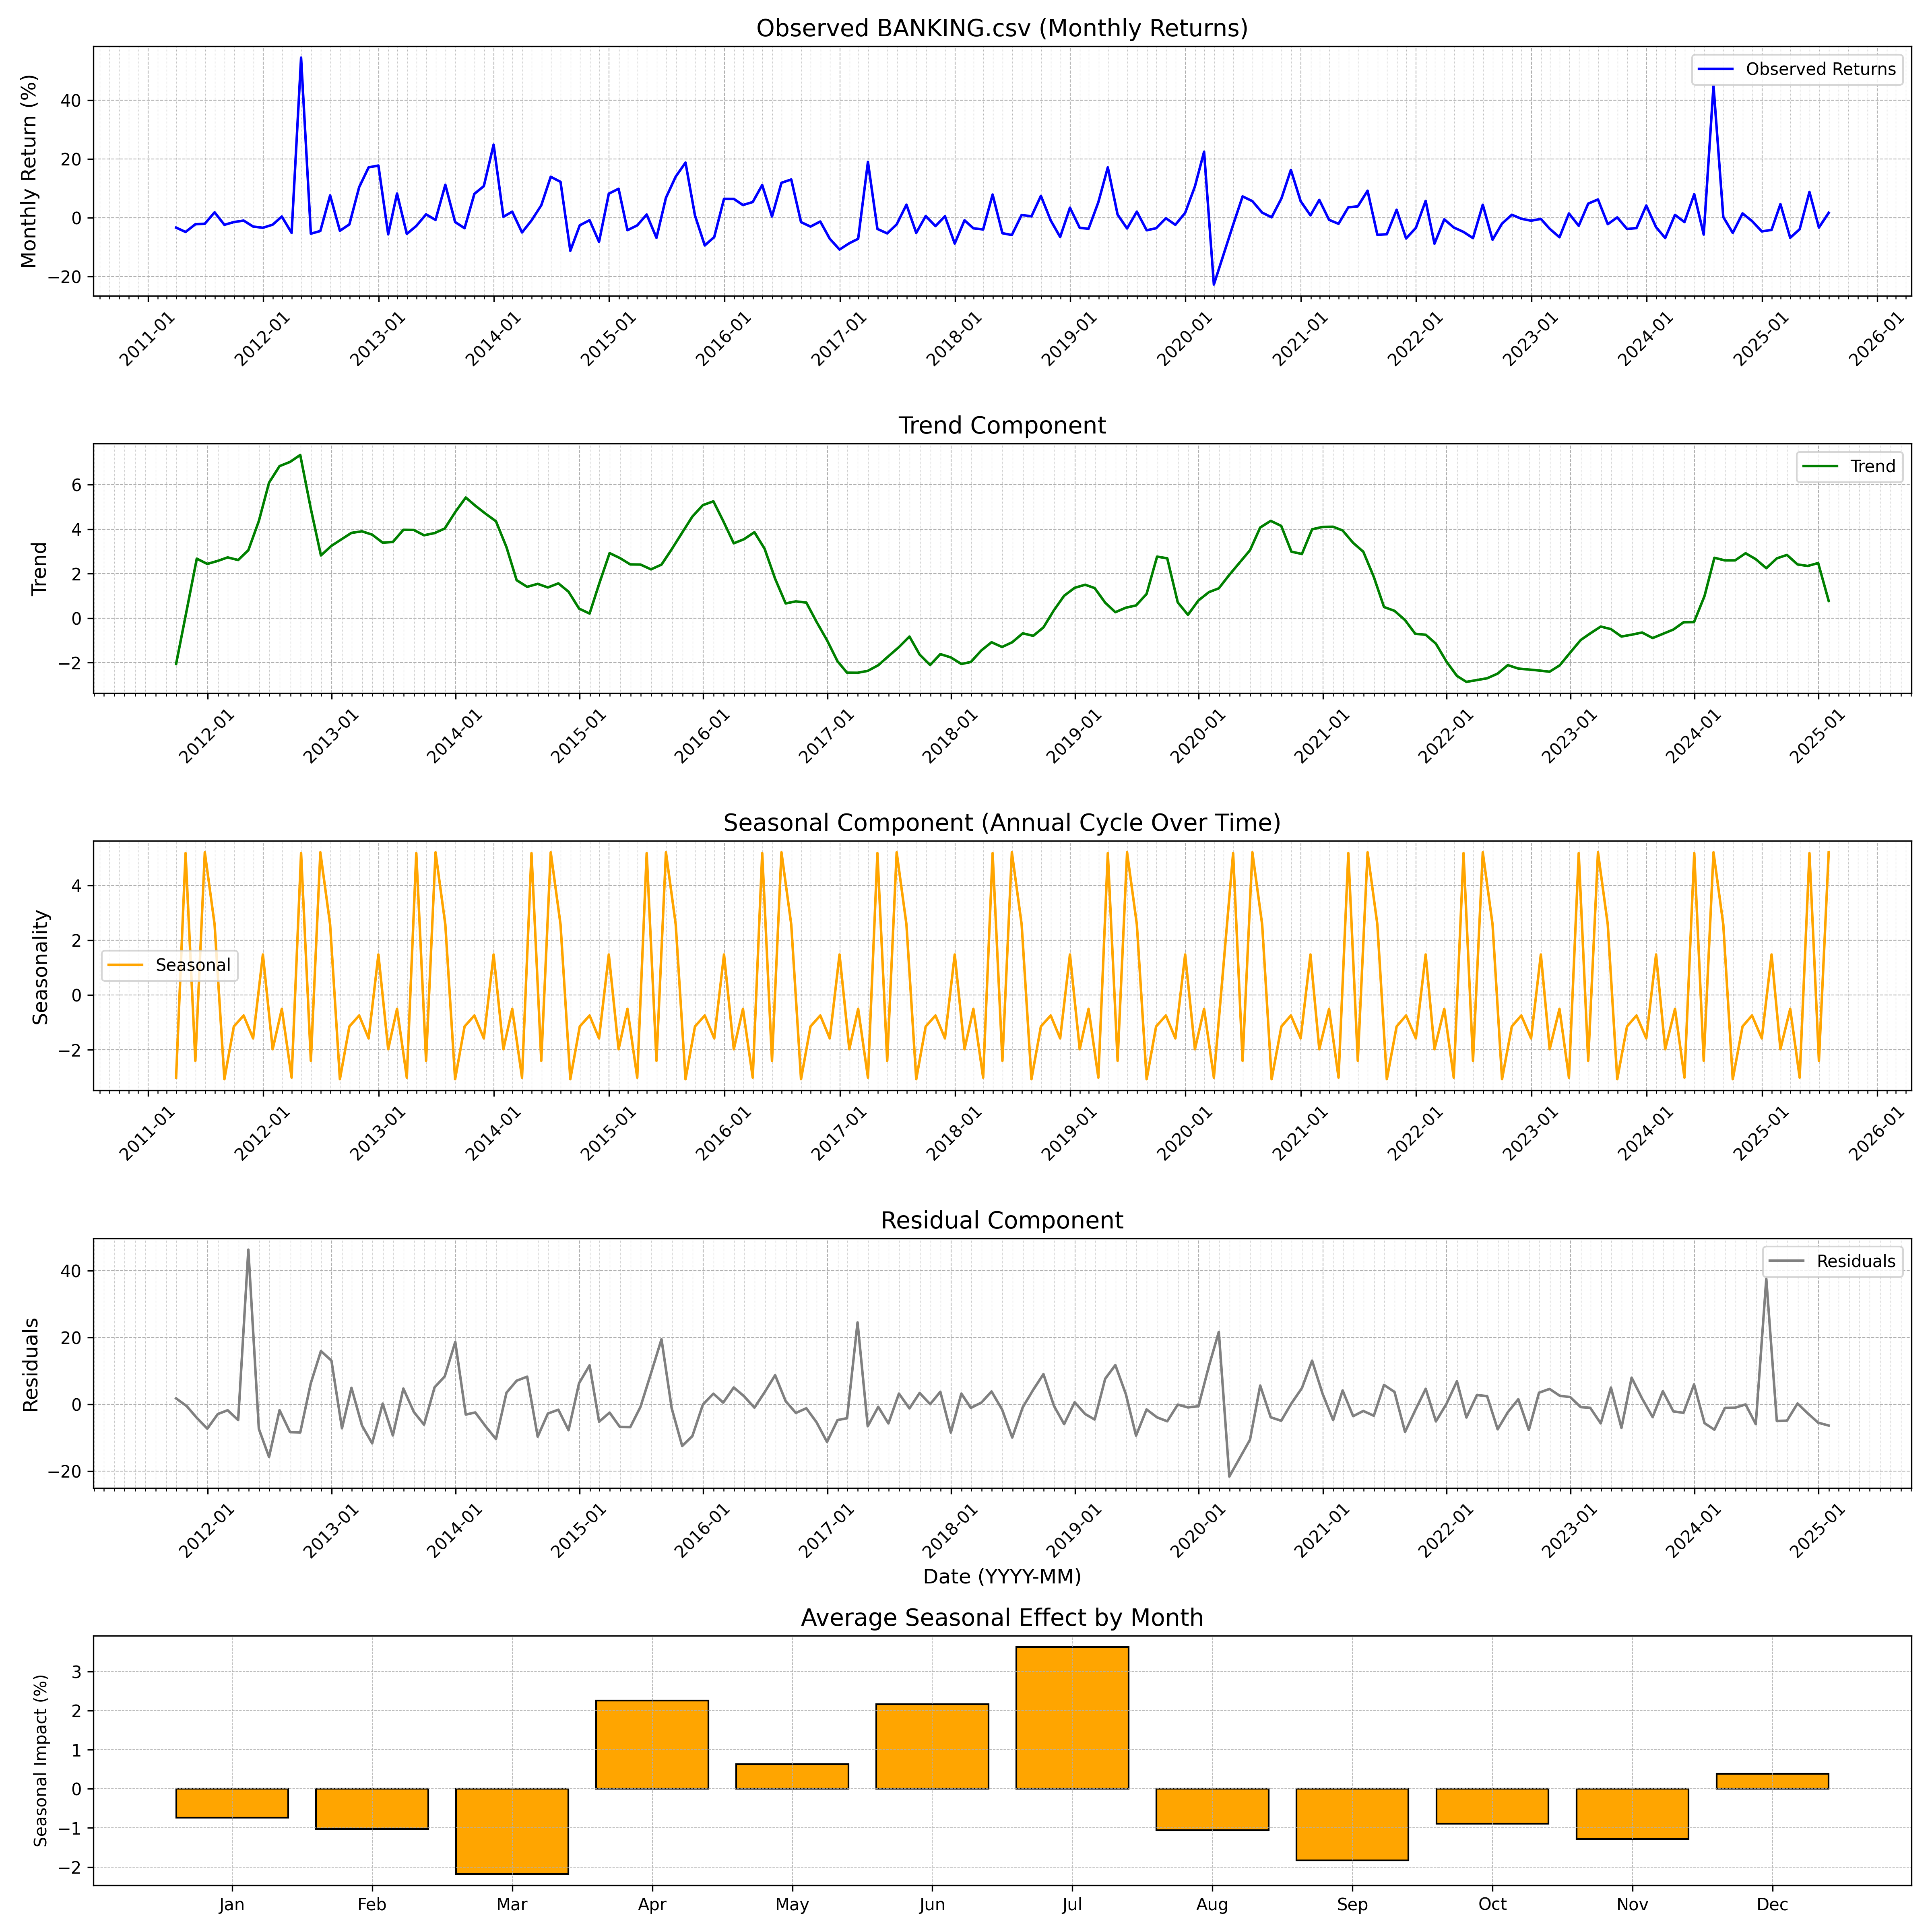
\includegraphics[width=0.9\textwidth]{decomposition_outputs/BANKING_seasonal_decomposition.png}
    \caption{Seasonal Decomposition of BANKING Index Monthly Returns}
\end{figure}

\begin{figure}[h!]
    \centering
    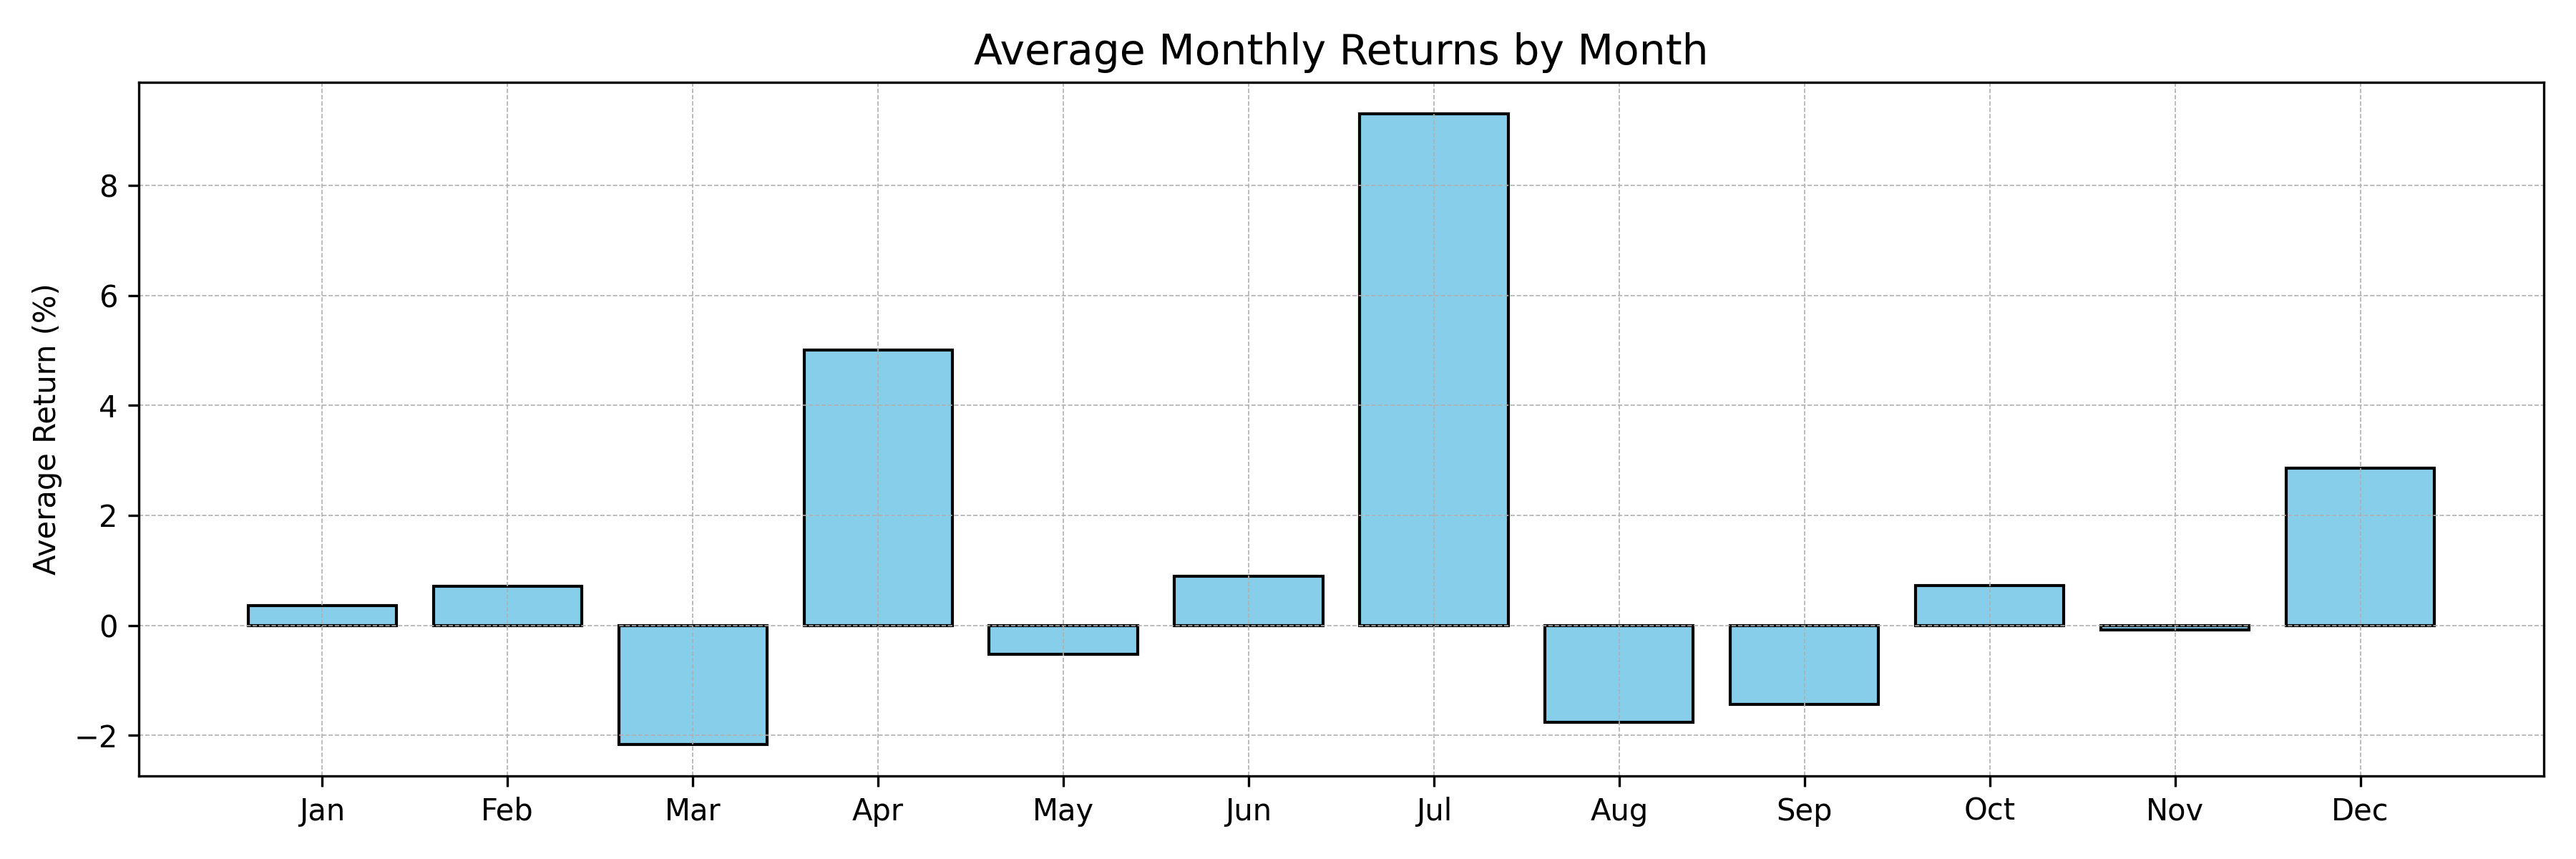
\includegraphics[width=0.7\textwidth]{decomposition_outputs/BANKING_avg_monthly_returns.png}
    \caption{Average Monthly Returns by Month -- BANKING}
\end{figure}

\begin{table}[h!]
\centering
\caption{Average Monthly Returns -- BANKING}
\begin{tabular}{l r}
\toprule
Month & Value (\%) \\
\midrule
Jan & 0.37 \\
Feb & 0.71 \\
Mar & -2.16 \\
Apr & 5.01 \\
May & -0.52 \\
Jun & 0.90 \\
Jul & 9.30 \\
Aug & -1.77 \\
Sep & -1.44 \\
Oct & 0.72 \\
Nov & -0.09 \\
Dec & 2.86 \\
\bottomrule
\end{tabular}
\end{table}

\begin{table}[h!]
\centering
\caption{Average Seasonality -- BANKING}
\begin{tabular}{l r}
\toprule
Month & Value (\%) \\
\midrule
Jan & -0.74 \\
Feb & -1.03 \\
Mar & -2.18 \\
Apr & 2.25 \\
May & 0.63 \\
Jun & 2.16 \\
Jul & 3.63 \\
Aug & -1.05 \\
Sep & -1.83 \\
Oct & -0.89 \\
Nov & -1.28 \\
Dec & 0.39 \\
\bottomrule
\end{tabular}
\end{table}


\clearpage

\subsection{DEVBANK}
\textbf{Mean Monthly Return:} 2.16\% \\
\textbf{Median Monthly Return:} 1.59\% \\
\textbf{Standard Deviation:} 3.31\% \\
\textbf{Best Month:} Jul (9.92\%) \\
\textbf{Worst Month:} Sep (-1.75\%) \\
\textbf{Seasonal Amplitude:} 11.67\% \\
\textbf{August Return:} -0.16\% \\

\begin{figure}[h!]
    \centering
    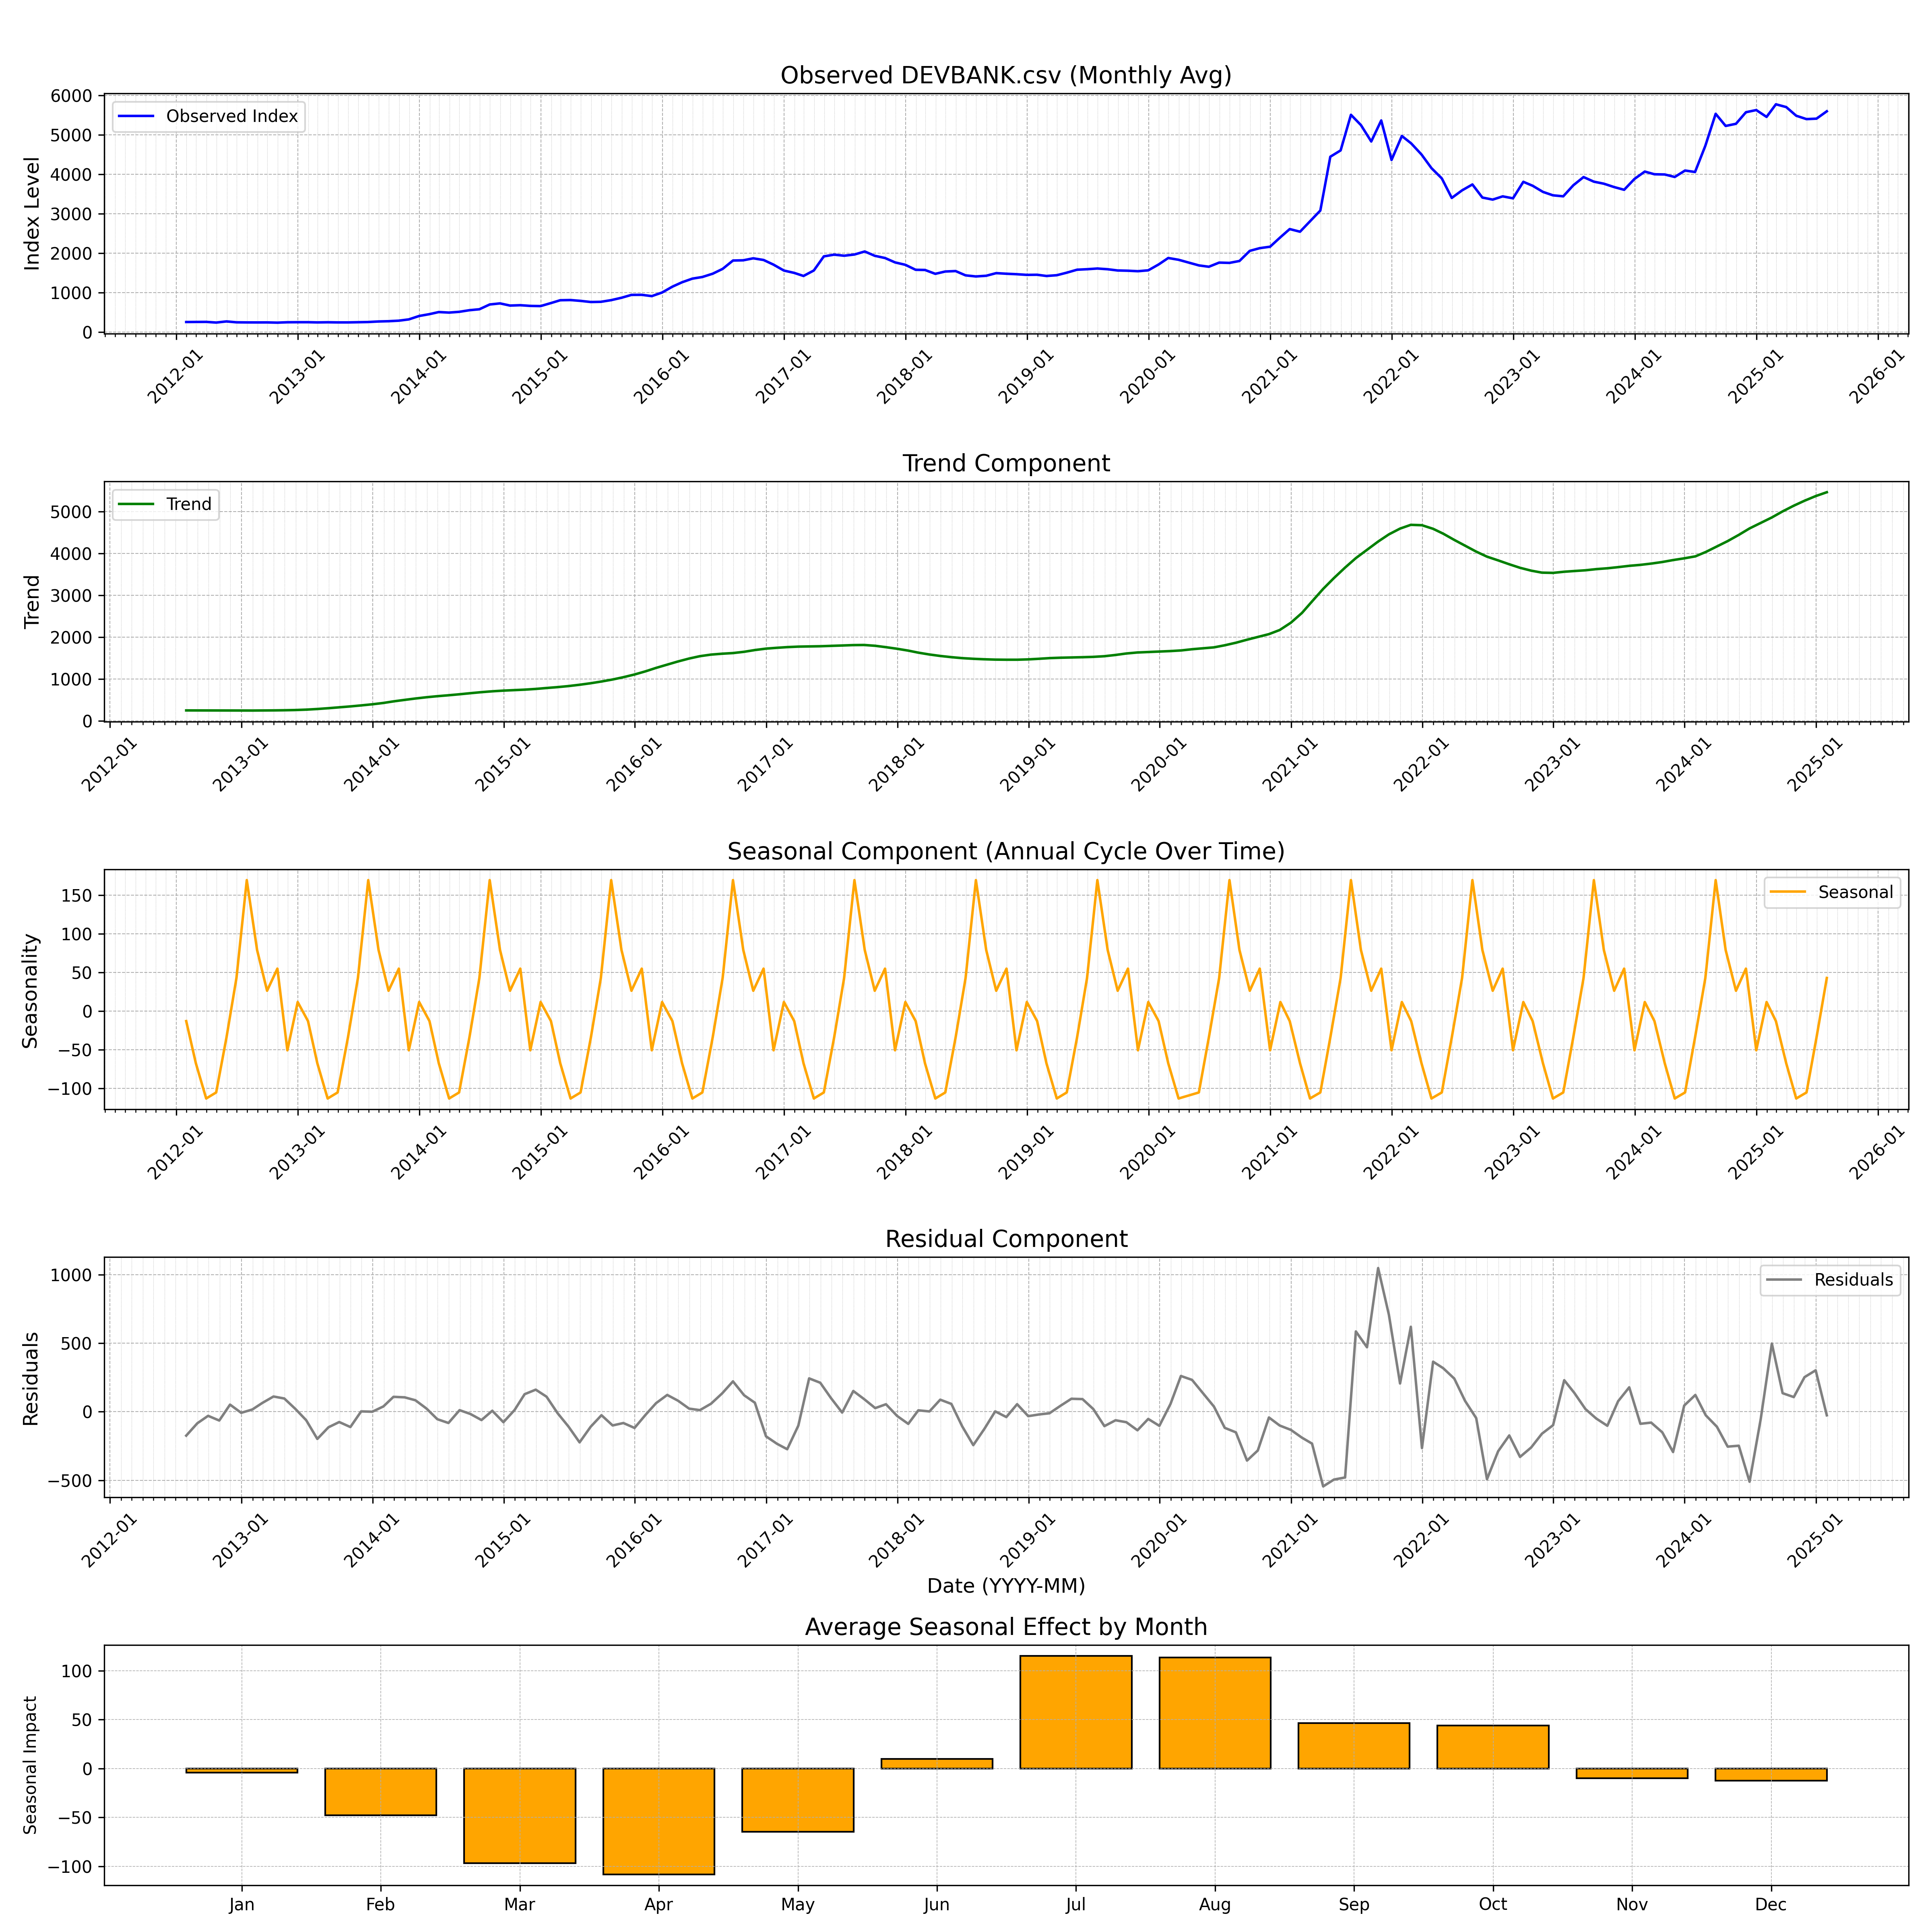
\includegraphics[width=0.9\textwidth]{decomposition_outputs/DEVBANK_seasonal_decomposition.png}
    \caption{Seasonal Decomposition of DEVBANK Index Monthly Returns}
\end{figure}

\begin{figure}[h!]
    \centering
    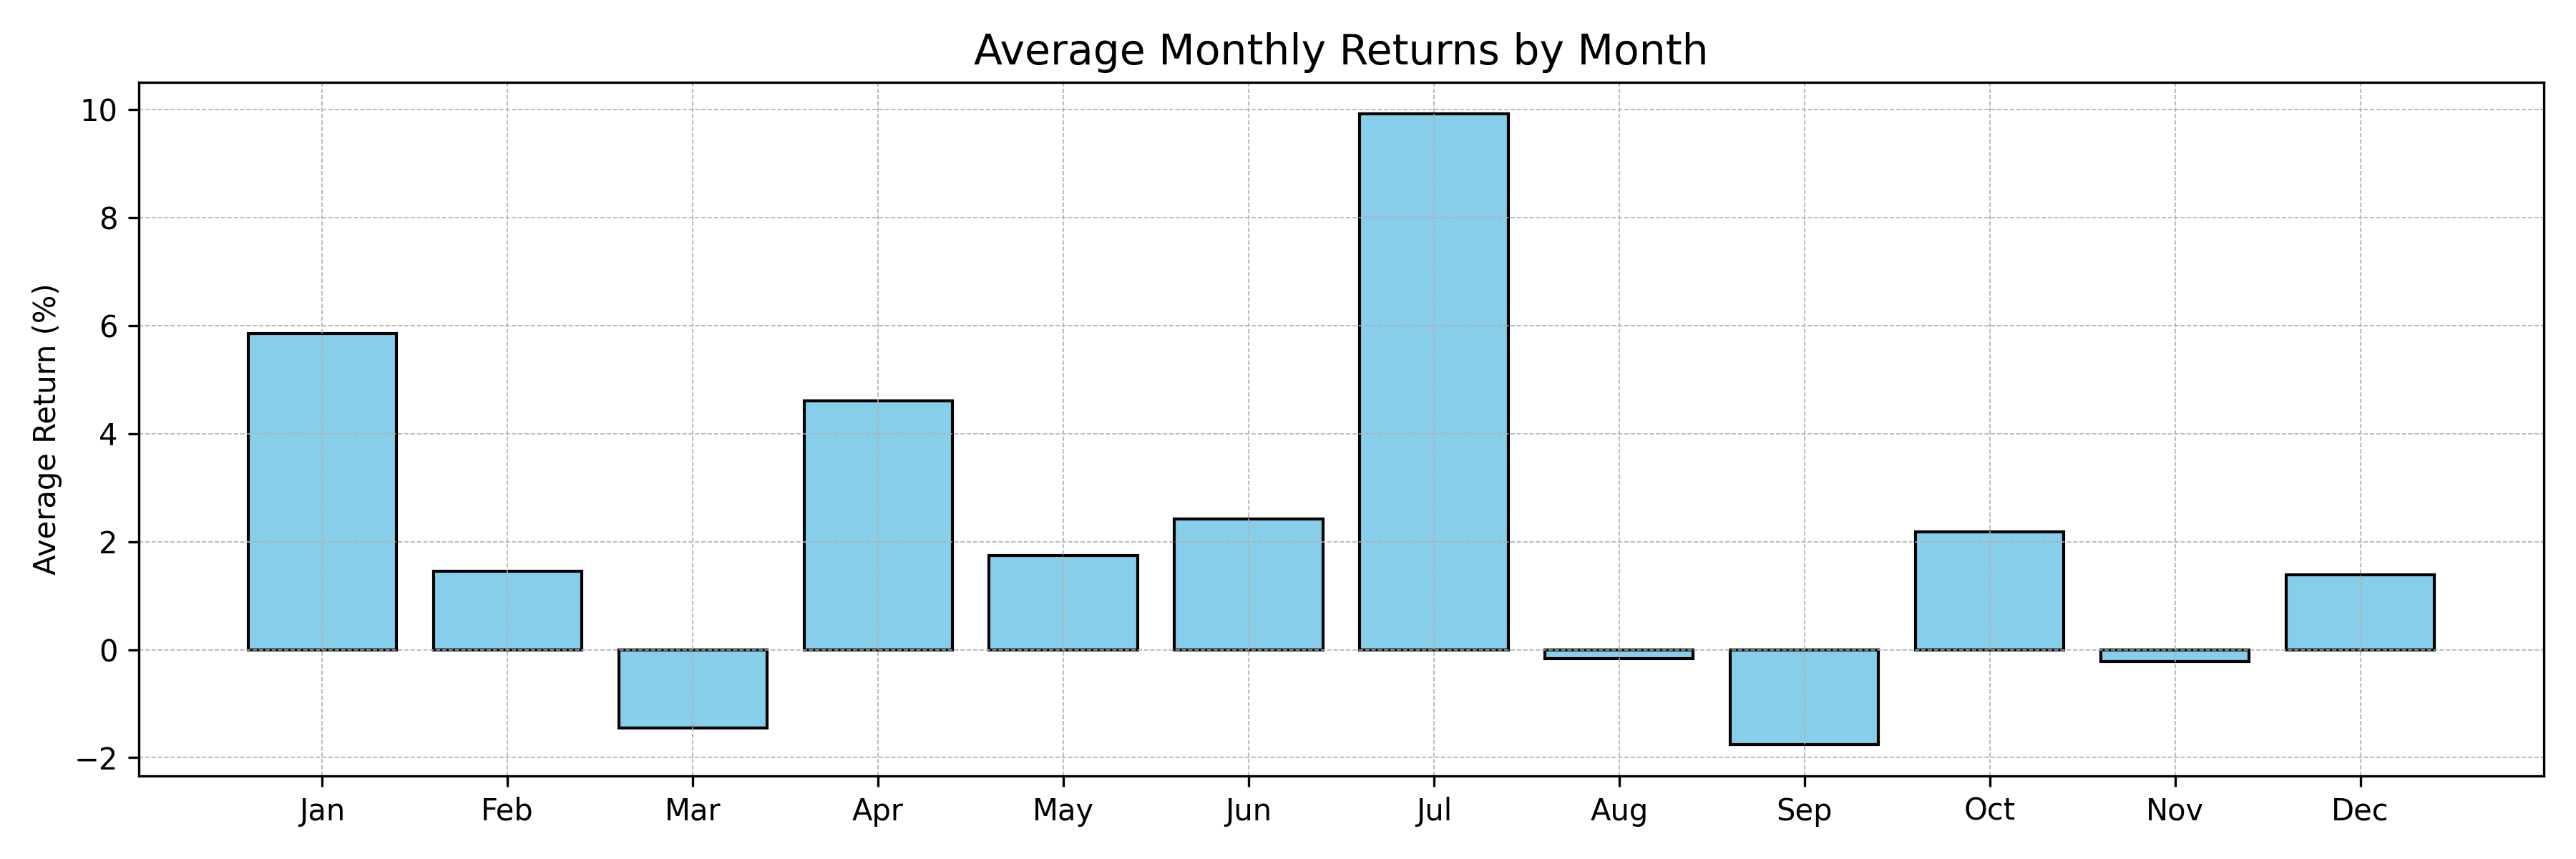
\includegraphics[width=0.7\textwidth]{decomposition_outputs/DEVBANK_avg_monthly_returns.png}
    \caption{Average Monthly Returns by Month -- DEVBANK}
\end{figure}

\begin{table}[h!]
\centering
\caption{Average Monthly Returns -- DEVBANK}
\begin{tabular}{l r}
\toprule
Month & Value (\%) \\
\midrule
Jan & 5.85 \\
Feb & 1.44 \\
Mar & -1.45 \\
Apr & 4.61 \\
May & 1.74 \\
Jun & 2.42 \\
Jul & 9.92 \\
Aug & -0.16 \\
Sep & -1.75 \\
Oct & 2.18 \\
Nov & -0.22 \\
Dec & 1.39 \\
\bottomrule
\end{tabular}
\end{table}

\begin{table}[h!]
\centering
\caption{Average Seasonality -- DEVBANK}
\begin{tabular}{l r}
\toprule
Month & Value (\%) \\
\midrule
Jan & 1.14 \\
Feb & -0.35 \\
Mar & -1.13 \\
Apr & 0.58 \\
May & 0.97 \\
Jun & 2.76 \\
Jul & 3.43 \\
Aug & -1.57 \\
Sep & -2.07 \\
Oct & -1.07 \\
Nov & -3.57 \\
Dec & 0.70 \\
\bottomrule
\end{tabular}
\end{table}


\clearpage

\subsection{FINANCE}
\textbf{Mean Monthly Return:} 1.48\% \\
\textbf{Median Monthly Return:} 0.84\% \\
\textbf{Standard Deviation:} 3.49\% \\
\textbf{Best Month:} Jul (10.05\%) \\
\textbf{Worst Month:} Sep (-2.78\%) \\
\textbf{Seasonal Amplitude:} 12.83\% \\
\textbf{August Return:} -1.93\% \\

\begin{figure}[h!]
    \centering
    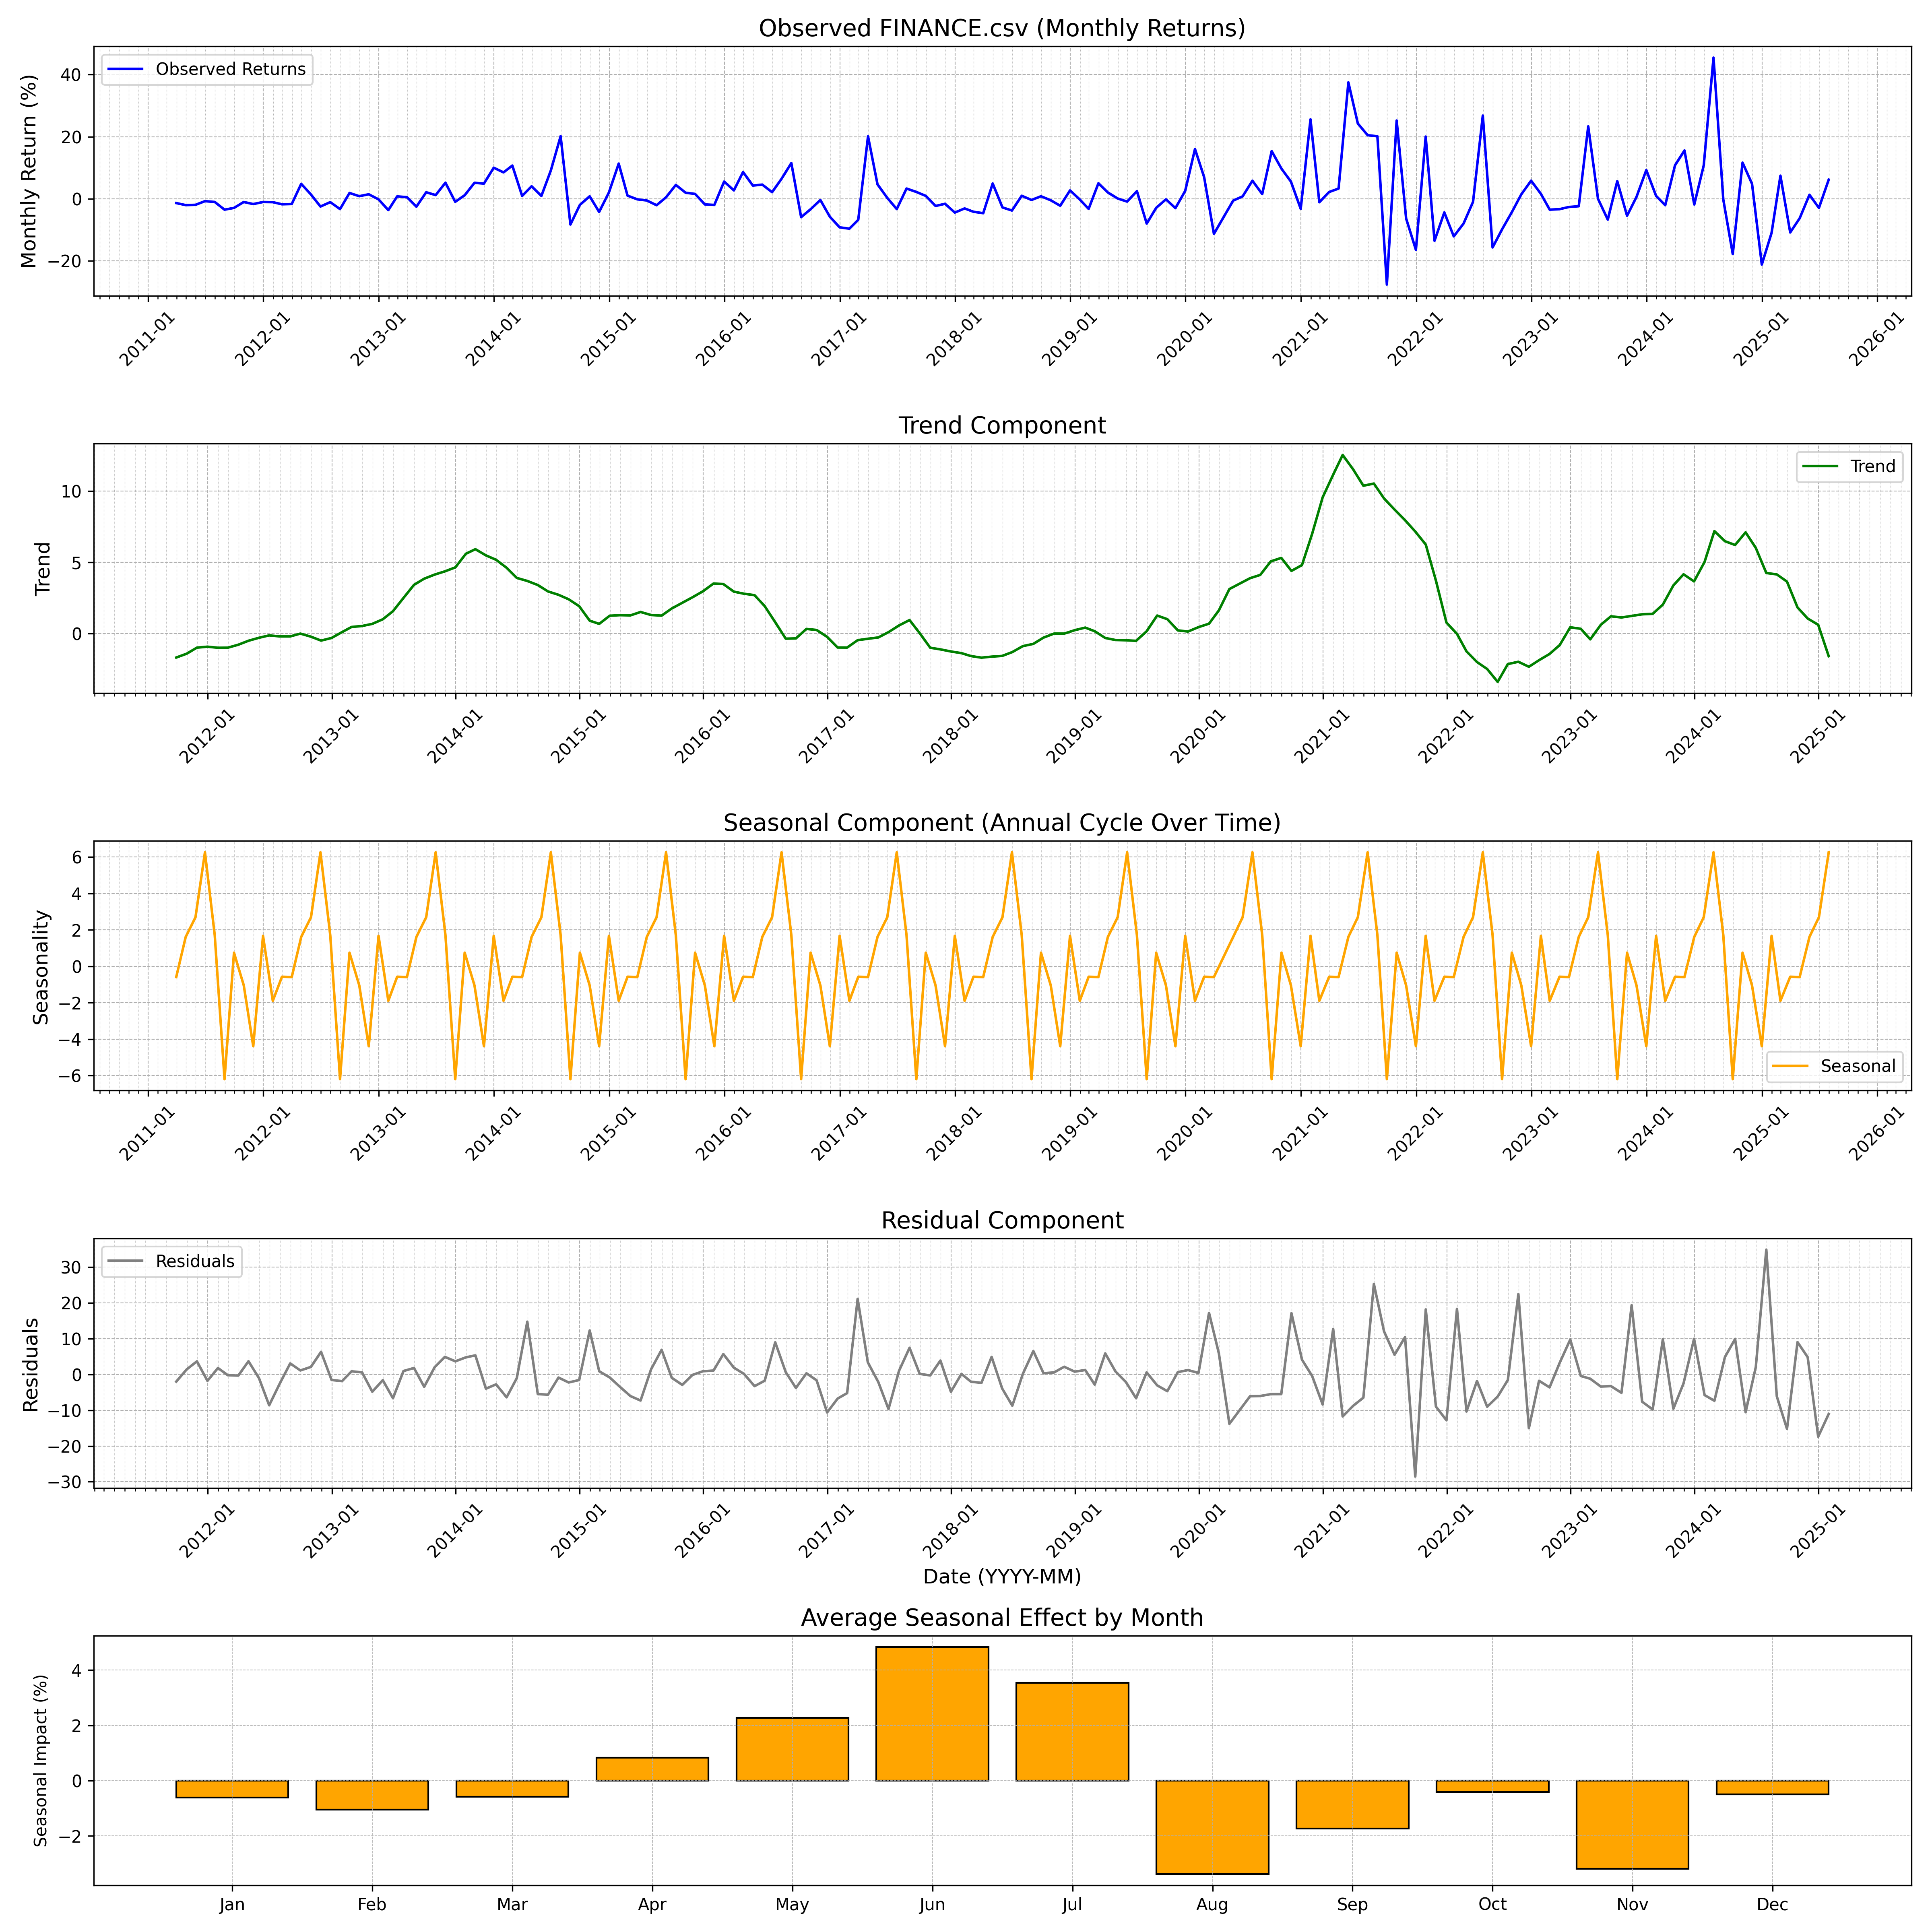
\includegraphics[width=0.9\textwidth]{decomposition_outputs/FINANCE_seasonal_decomposition.png}
    \caption{Seasonal Decomposition of FINANCE Index Monthly Returns}
\end{figure}

\begin{figure}[h!]
    \centering
    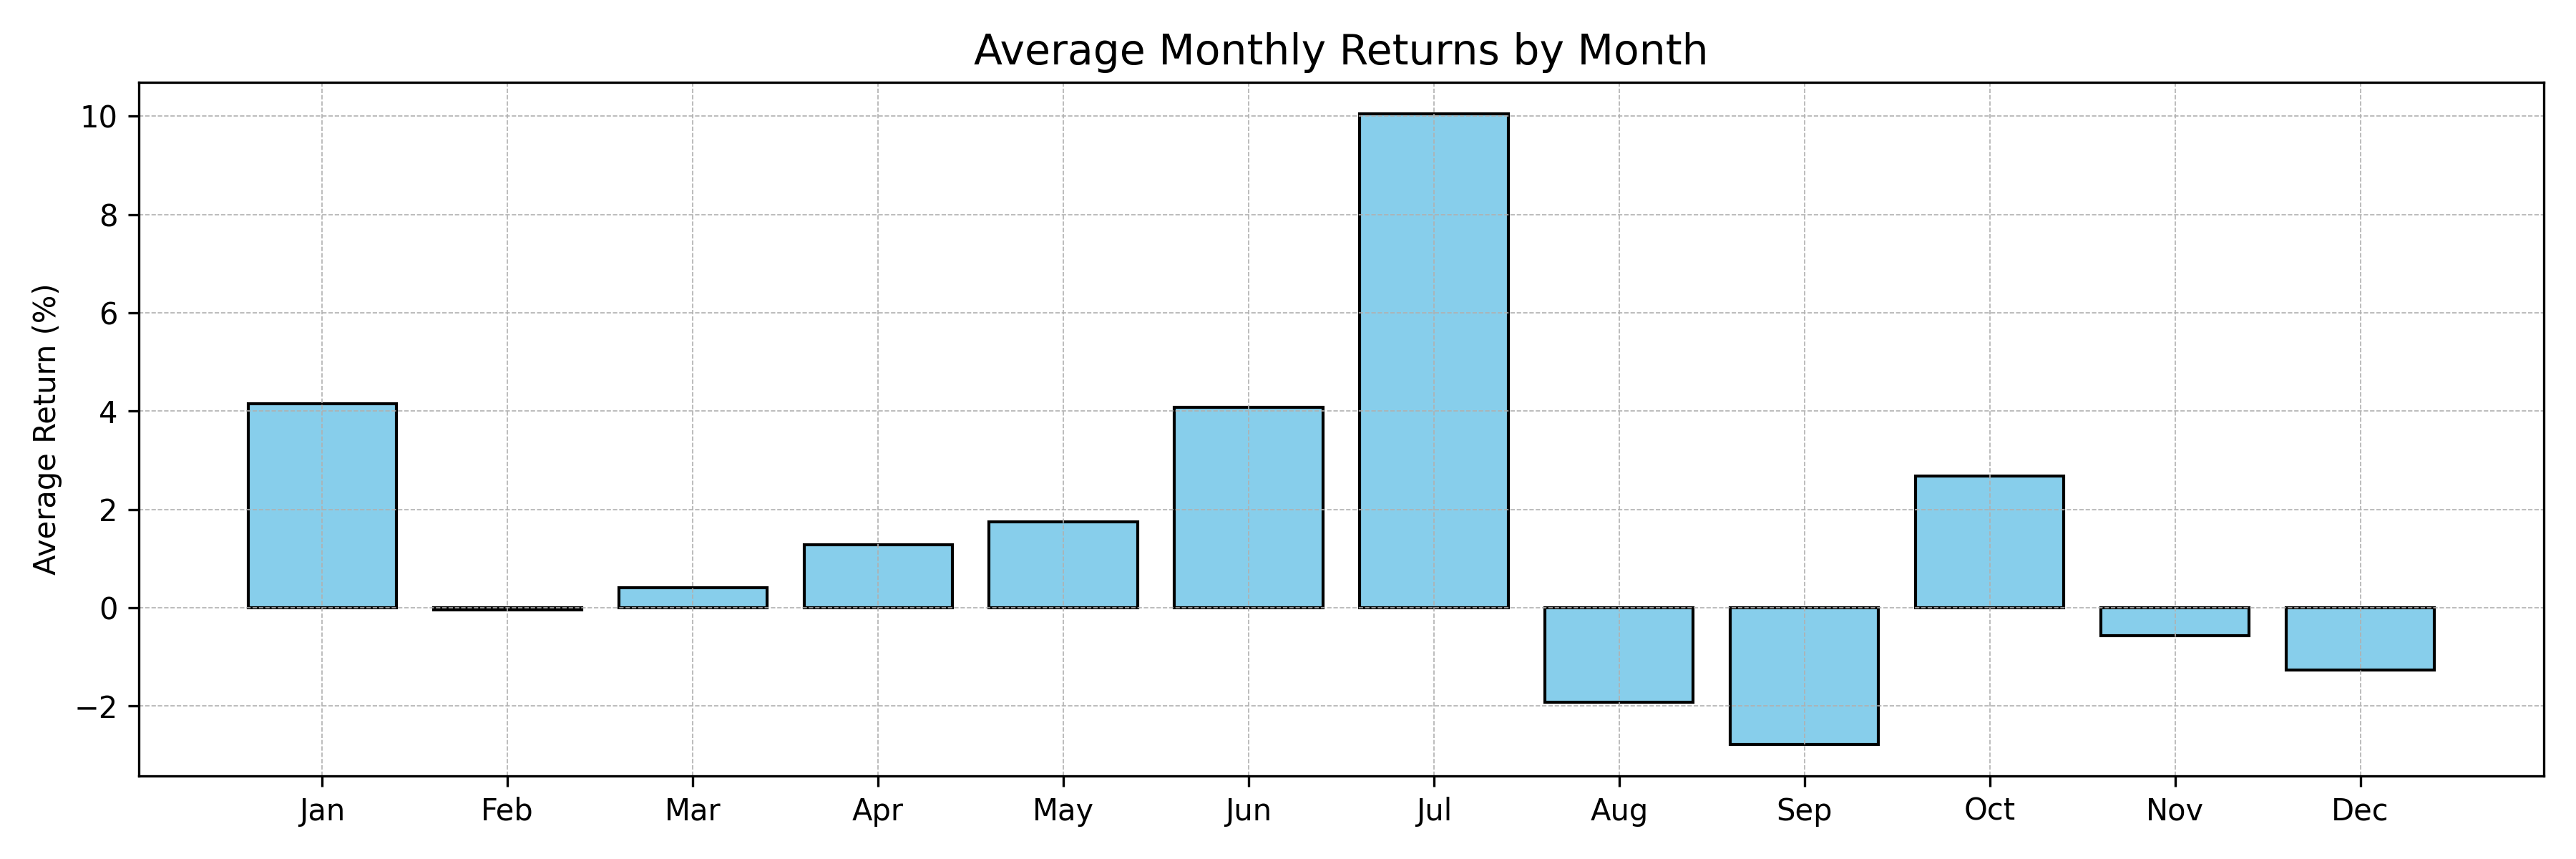
\includegraphics[width=0.7\textwidth]{decomposition_outputs/FINANCE_avg_monthly_returns.png}
    \caption{Average Monthly Returns by Month -- FINANCE}
\end{figure}

\begin{table}[h!]
\centering
\caption{Average Monthly Returns -- FINANCE}
\begin{tabular}{l r}
\toprule
Month & Value (\%) \\
\midrule
Jan & 4.15 \\
Feb & -0.04 \\
Mar & 0.41 \\
Apr & 1.28 \\
May & 1.75 \\
Jun & 4.08 \\
Jul & 10.05 \\
Aug & -1.93 \\
Sep & -2.78 \\
Oct & 2.68 \\
Nov & -0.57 \\
Dec & -1.26 \\
\bottomrule
\end{tabular}
\end{table}

\begin{table}[h!]
\centering
\caption{Average Seasonality -- FINANCE}
\begin{tabular}{l r}
\toprule
Month & Value (\%) \\
\midrule
Jan & -0.62 \\
Feb & -1.05 \\
Mar & -0.58 \\
Apr & 0.83 \\
May & 2.26 \\
Jun & 4.83 \\
Jul & 3.53 \\
Aug & -3.38 \\
Sep & -1.73 \\
Oct & -0.41 \\
Nov & -3.20 \\
Dec & -0.49 \\
\bottomrule
\end{tabular}
\end{table}


\clearpage

\subsection{HOTELS}
\textbf{Mean Monthly Return:} 1.76\% \\
\textbf{Median Monthly Return:} 1.84\% \\
\textbf{Standard Deviation:} 2.75\% \\
\textbf{Best Month:} Jul (6.40\%) \\
\textbf{Worst Month:} Aug (-2.52\%) \\
\textbf{Seasonal Amplitude:} 8.92\% \\
\textbf{August Return:} -2.52\% \\

\begin{figure}[h!]
    \centering
    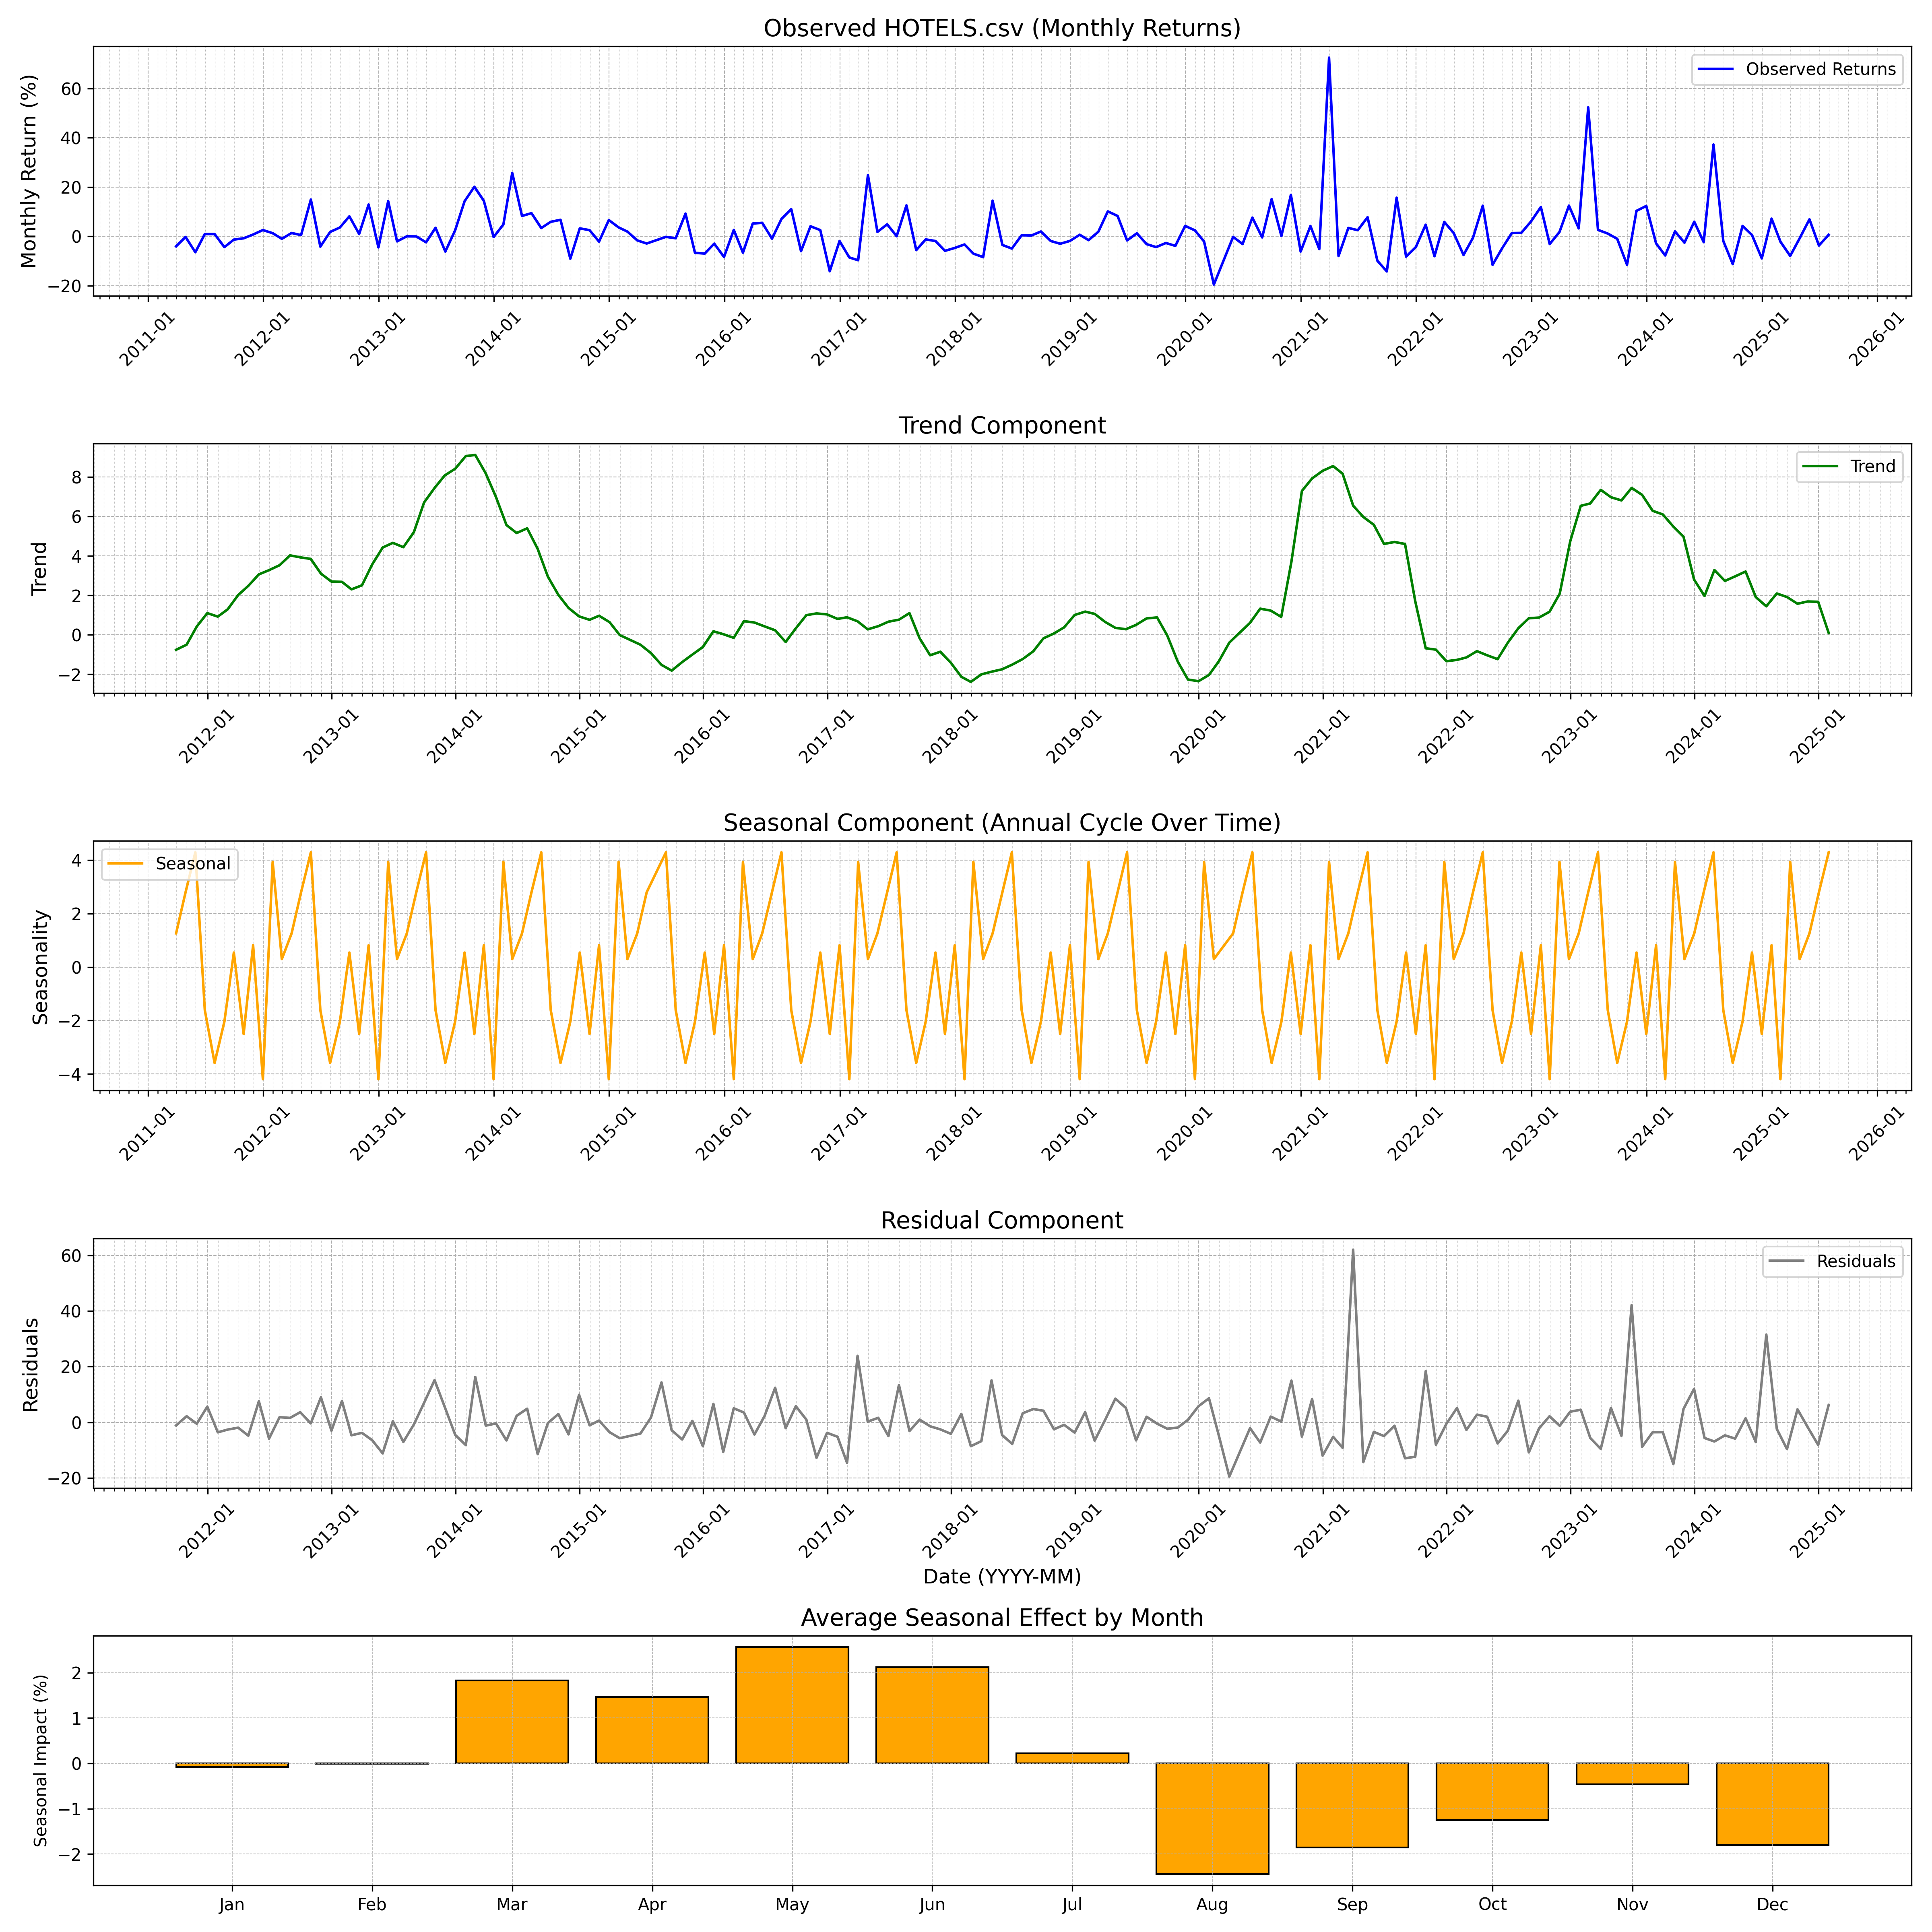
\includegraphics[width=0.9\textwidth]{decomposition_outputs/HOTELS_seasonal_decomposition.png}
    \caption{Seasonal Decomposition of HOTELS Index Monthly Returns}
\end{figure}

\begin{figure}[h!]
    \centering
    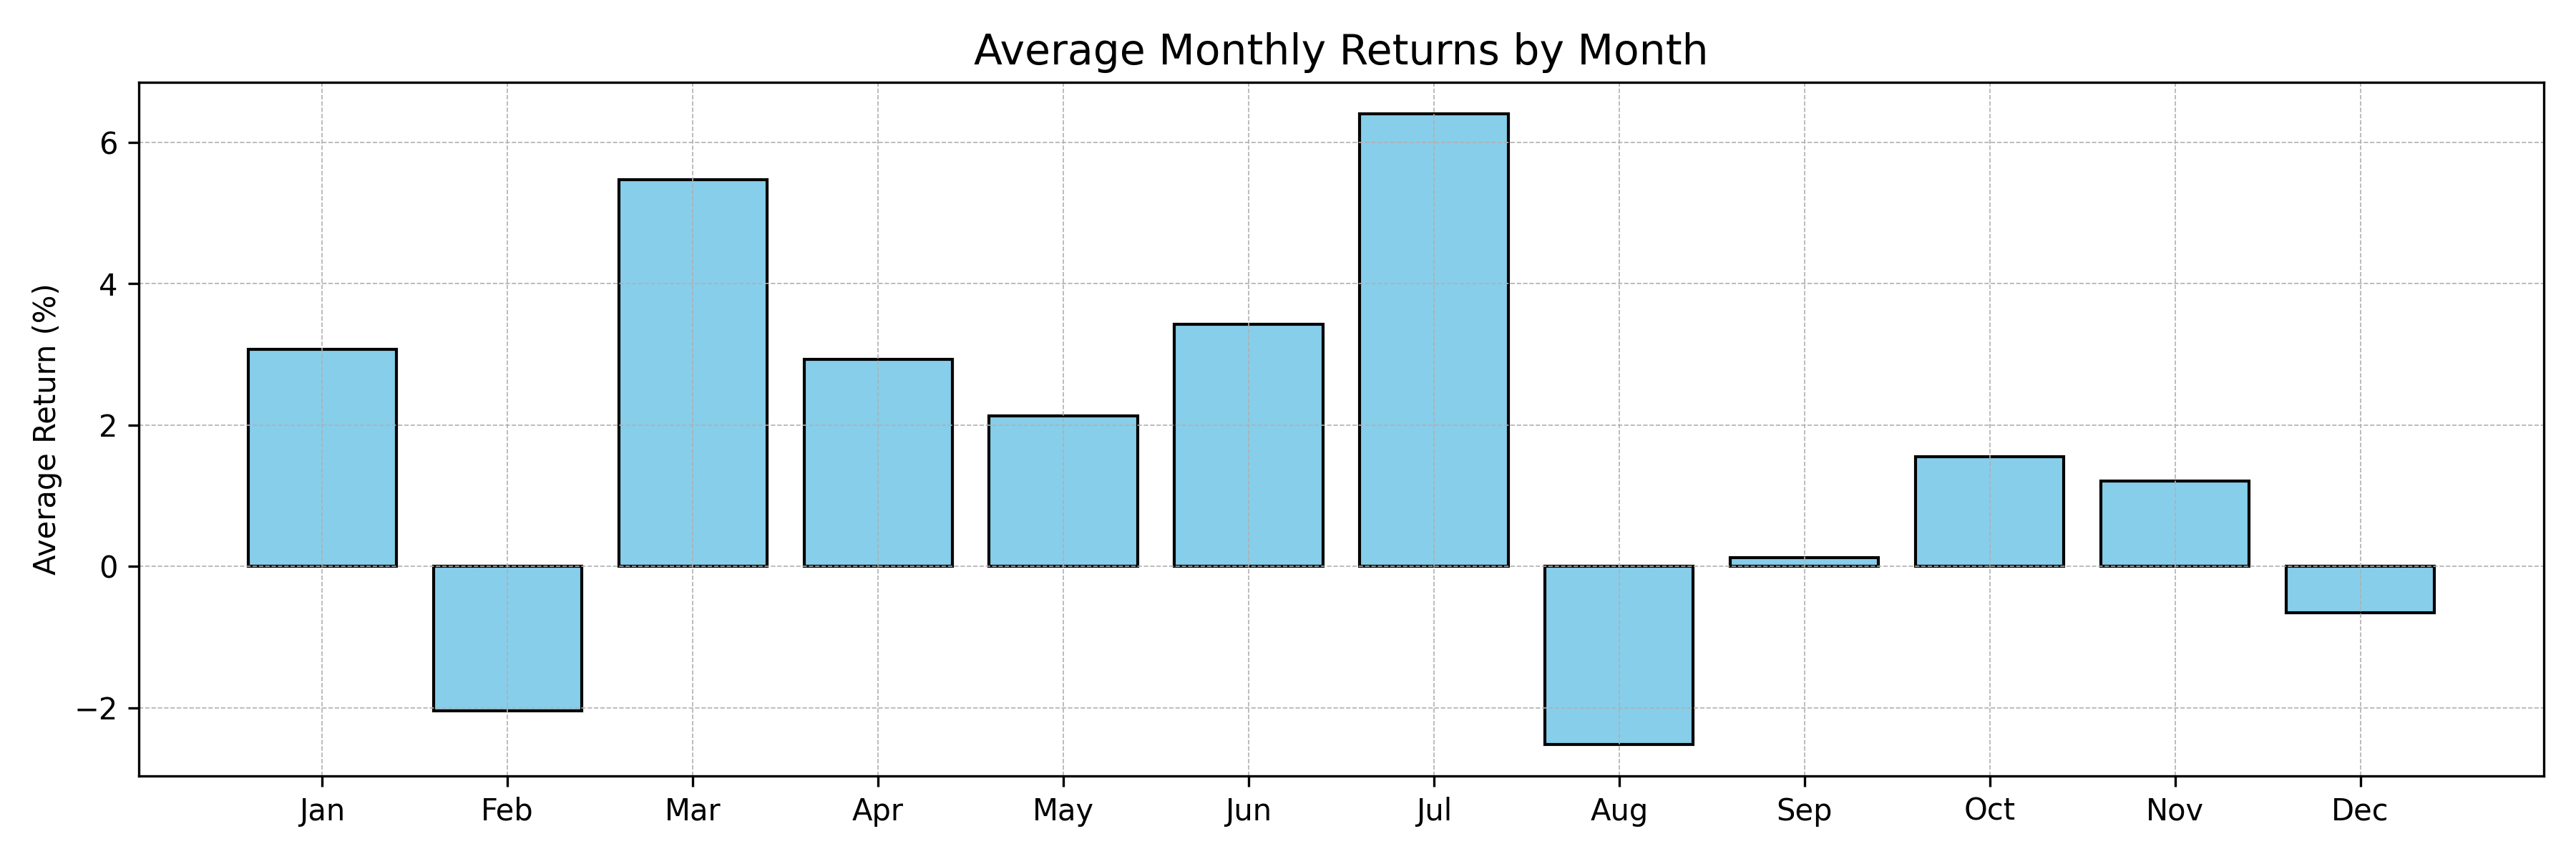
\includegraphics[width=0.7\textwidth]{decomposition_outputs/HOTELS_avg_monthly_returns.png}
    \caption{Average Monthly Returns by Month -- HOTELS}
\end{figure}

\begin{table}[h!]
\centering
\caption{Average Monthly Returns -- HOTELS}
\begin{tabular}{l r}
\toprule
Month & Value (\%) \\
\midrule
Jan & 3.07 \\
Feb & -2.05 \\
Mar & 5.47 \\
Apr & 2.93 \\
May & 2.13 \\
Jun & 3.43 \\
Jul & 6.40 \\
Aug & -2.52 \\
Sep & 0.12 \\
Oct & 1.55 \\
Nov & 1.21 \\
Dec & -0.66 \\
\bottomrule
\end{tabular}
\end{table}

\begin{table}[h!]
\centering
\caption{Average Seasonality -- HOTELS}
\begin{tabular}{l r}
\toprule
Month & Value (\%) \\
\midrule
Jan & -0.08 \\
Feb & -0.01 \\
Mar & 1.83 \\
Apr & 1.47 \\
May & 2.57 \\
Jun & 2.12 \\
Jul & 0.22 \\
Aug & -2.44 \\
Sep & -1.86 \\
Oct & -1.25 \\
Nov & -0.47 \\
Dec & -1.80 \\
\bottomrule
\end{tabular}
\end{table}


\clearpage

\subsection{HYDROPOWER}
\textbf{Mean Monthly Return:} 1.47\% \\
\textbf{Median Monthly Return:} 0.93\% \\
\textbf{Standard Deviation:} 2.93\% \\
\textbf{Best Month:} Jan (6.78\%) \\
\textbf{Worst Month:} Aug (-3.06\%) \\
\textbf{Seasonal Amplitude:} 9.84\% \\
\textbf{August Return:} -3.06\% \\

\begin{figure}[h!]
    \centering
    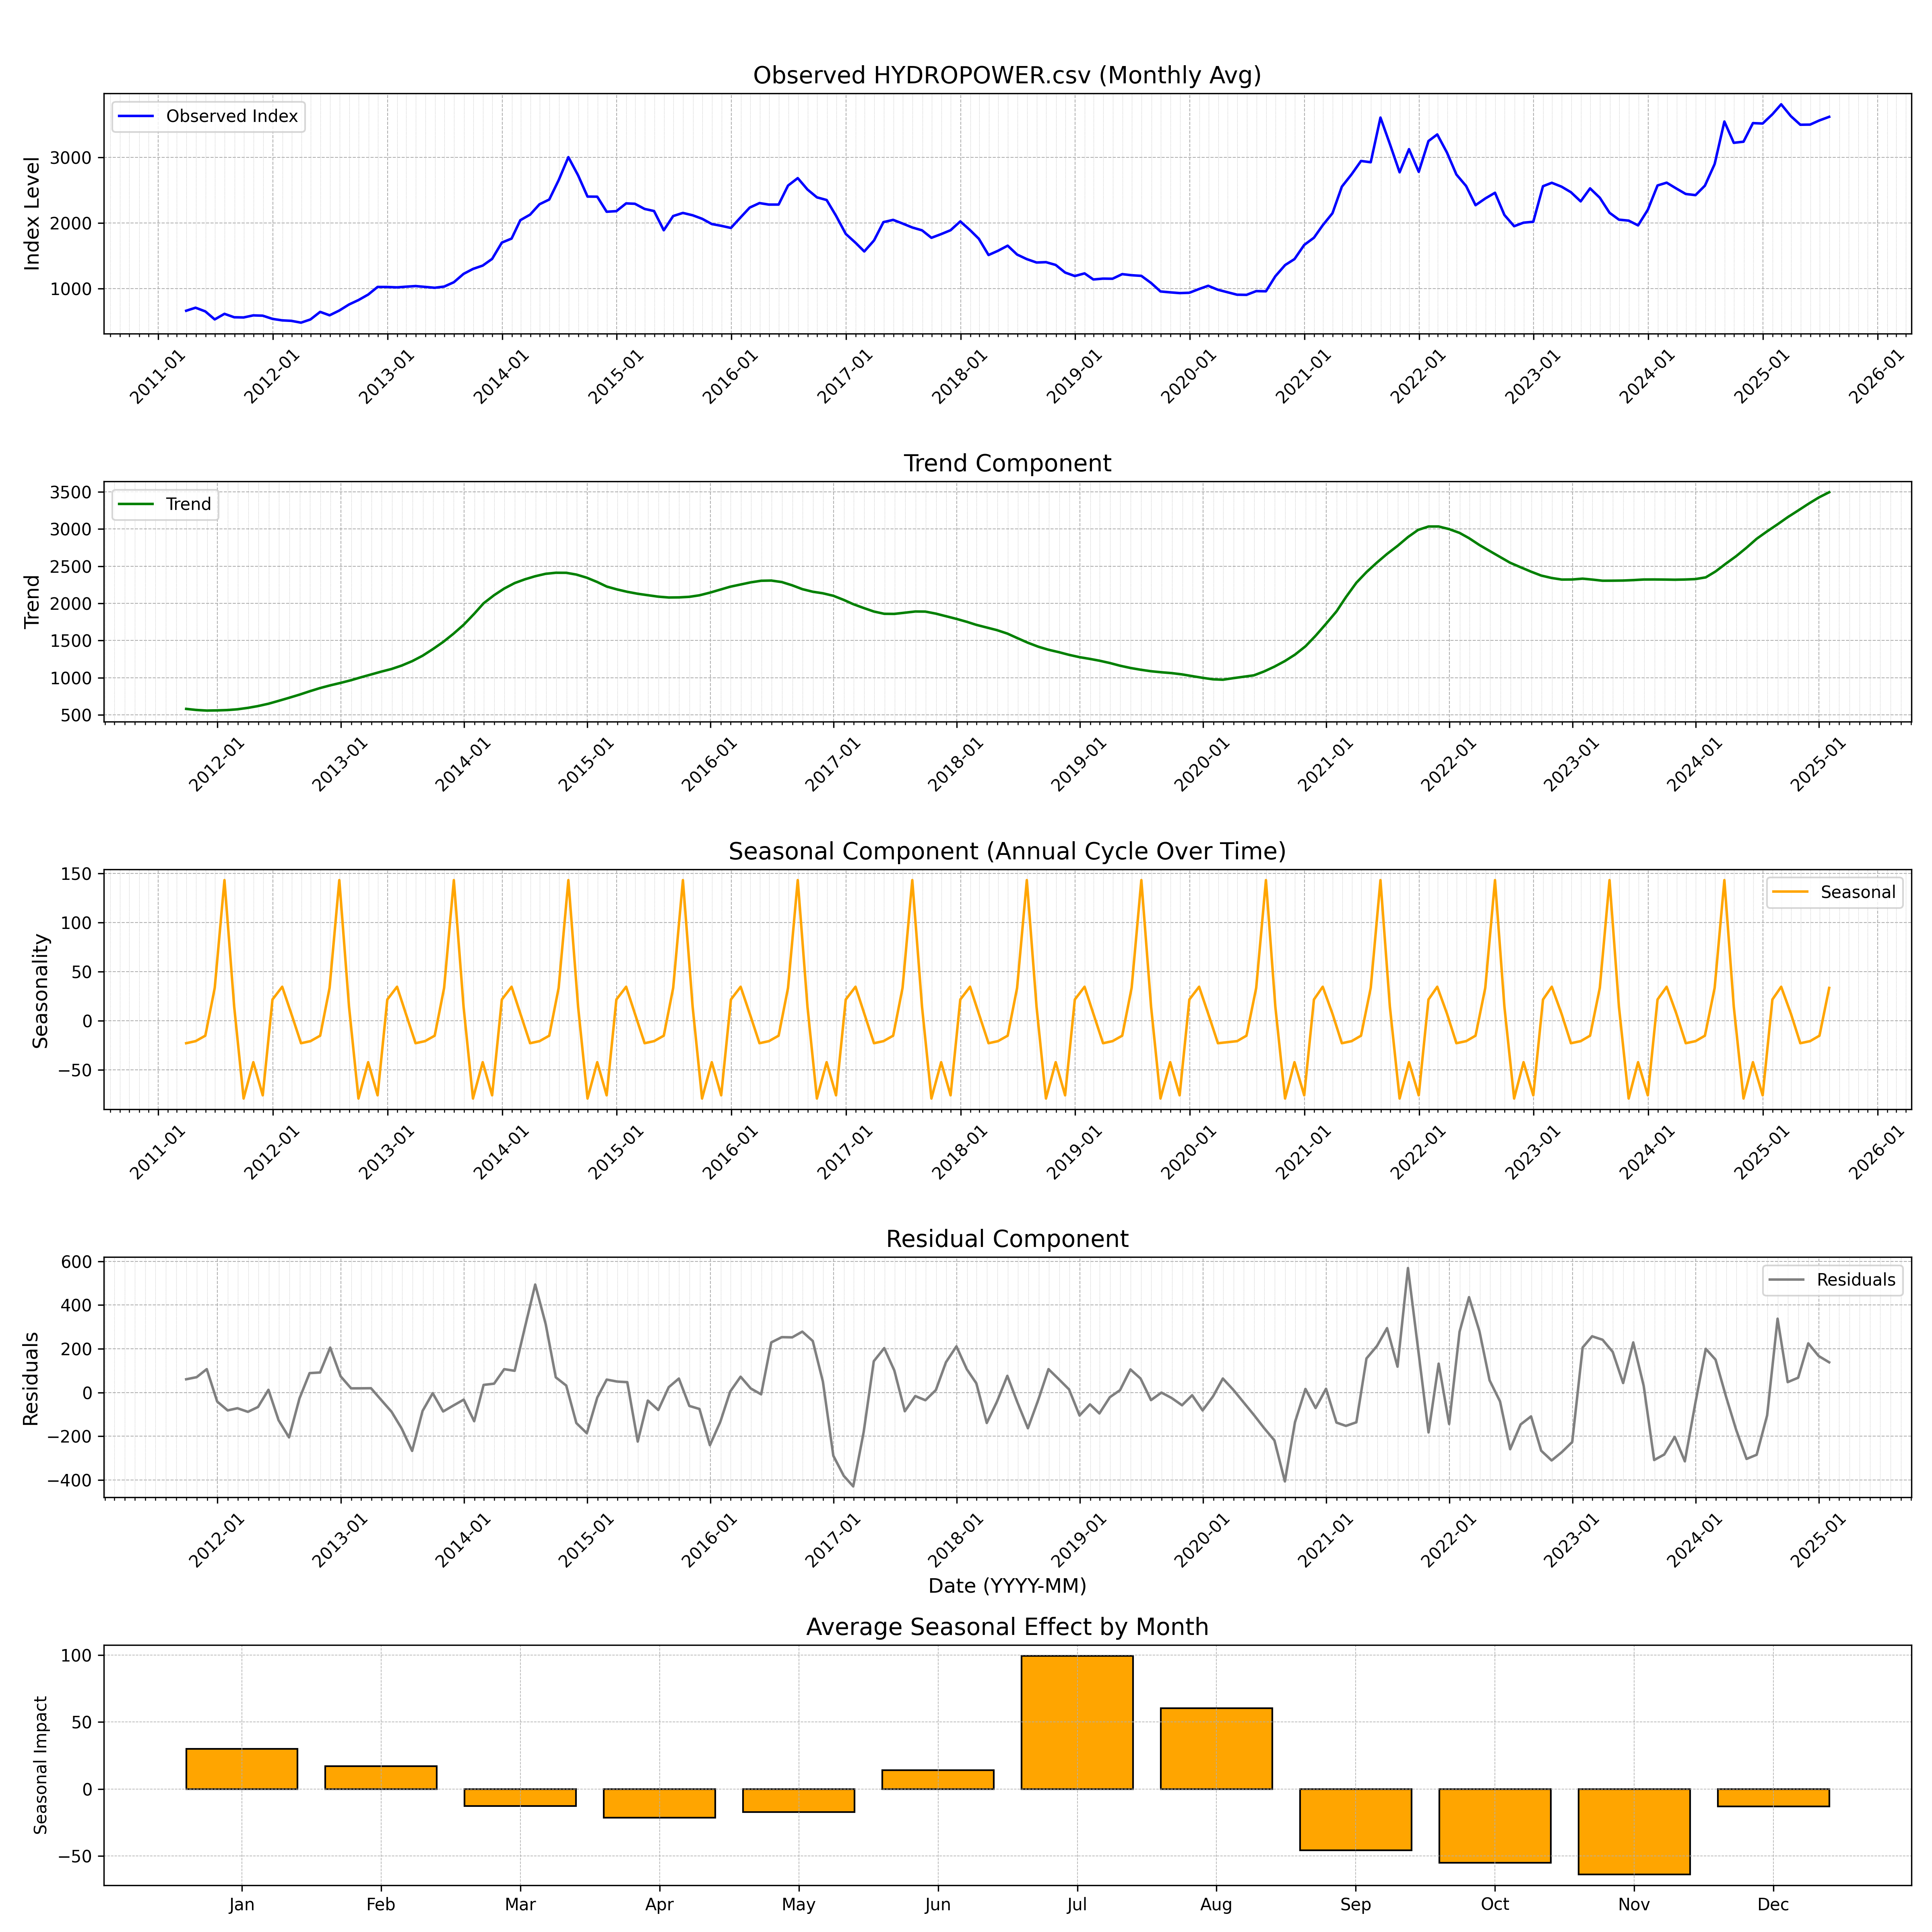
\includegraphics[width=0.9\textwidth]{decomposition_outputs/HYDROPOWER_seasonal_decomposition.png}
    \caption{Seasonal Decomposition of HYDROPOWER Index Monthly Returns}
\end{figure}

\begin{figure}[h!]
    \centering
    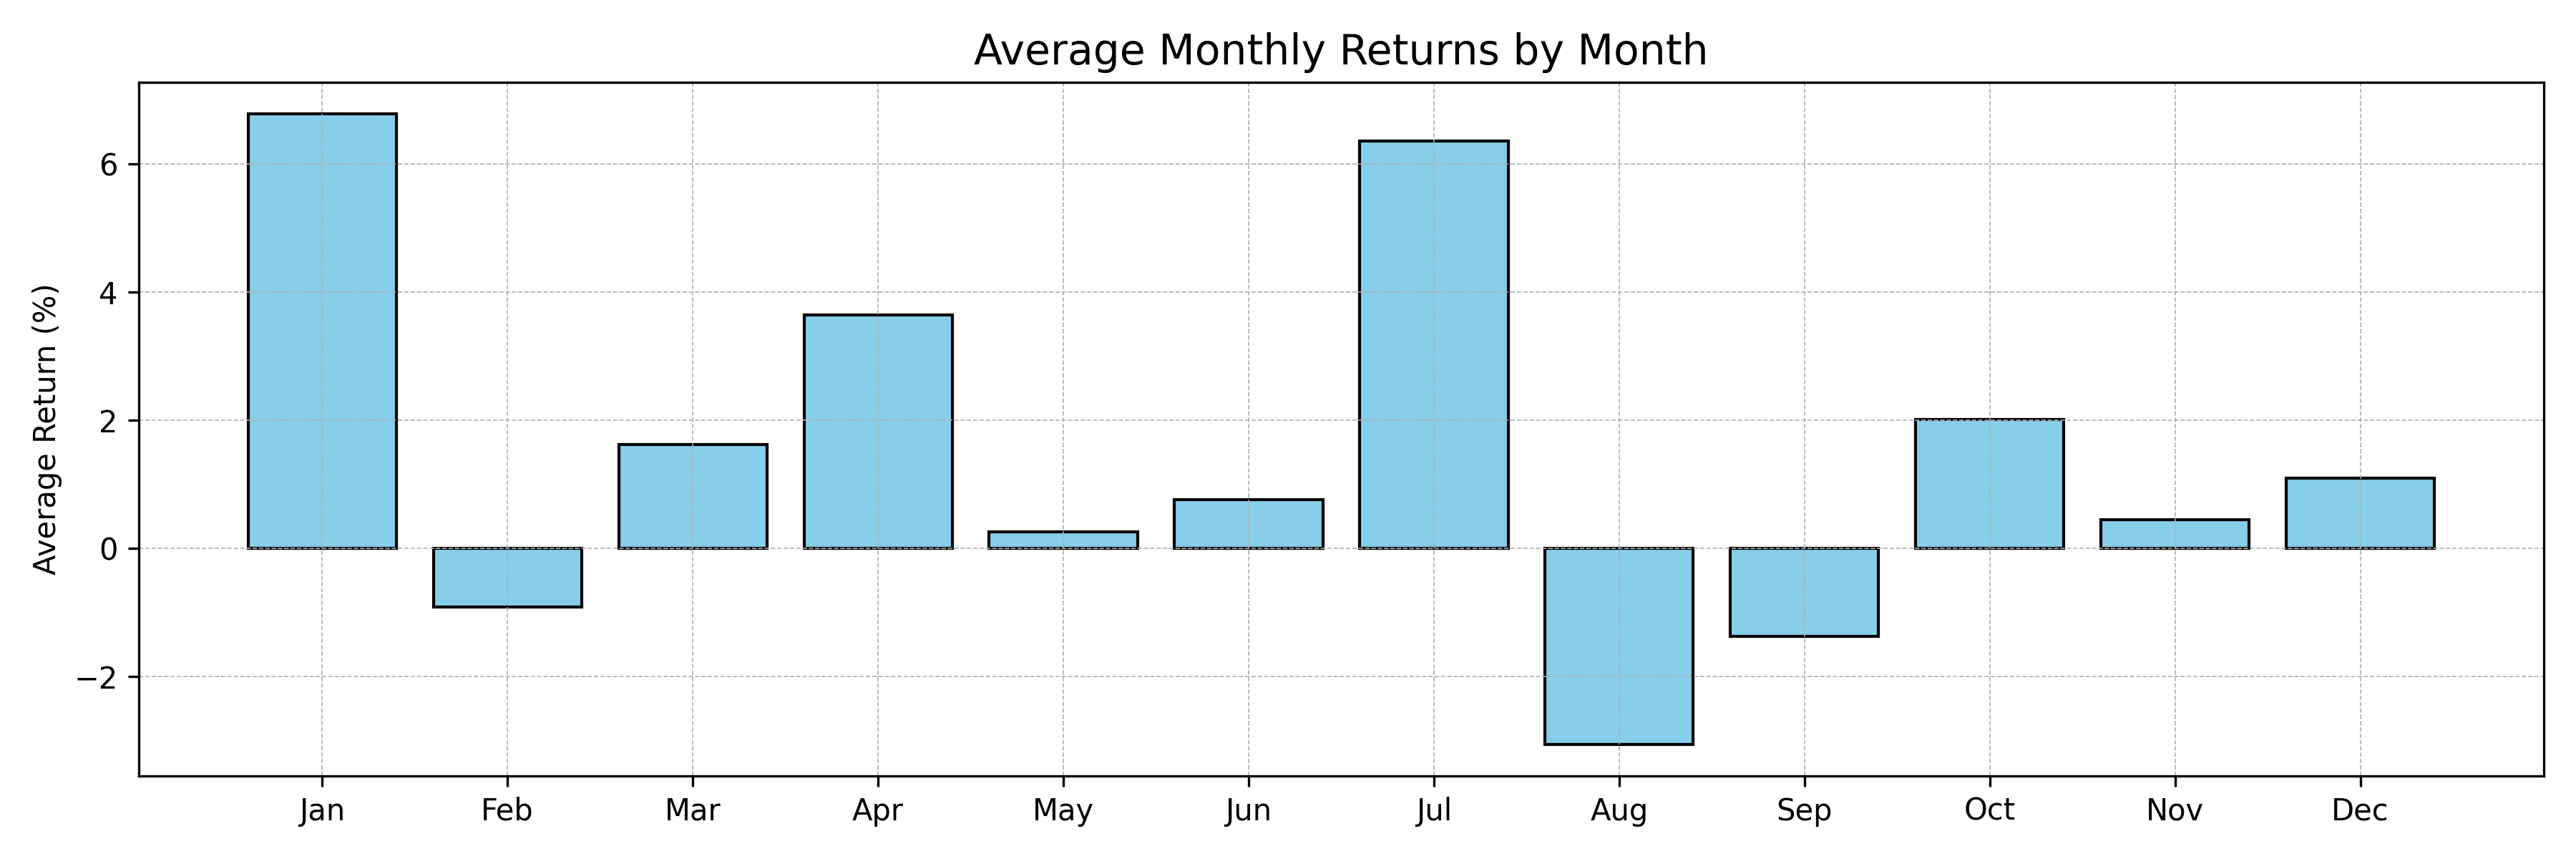
\includegraphics[width=0.7\textwidth]{decomposition_outputs/HYDROPOWER_avg_monthly_returns.png}
    \caption{Average Monthly Returns by Month -- HYDROPOWER}
\end{figure}

\begin{table}[h!]
\centering
\caption{Average Monthly Returns -- HYDROPOWER}
\begin{tabular}{l r}
\toprule
Month & Value (\%) \\
\midrule
Jan & 6.78 \\
Feb & -0.91 \\
Mar & 1.62 \\
Apr & 3.64 \\
May & 0.26 \\
Jun & 0.76 \\
Jul & 6.36 \\
Aug & -3.06 \\
Sep & -1.37 \\
Oct & 2.01 \\
Nov & 0.45 \\
Dec & 1.10 \\
\bottomrule
\end{tabular}
\end{table}

\begin{table}[h!]
\centering
\caption{Average Seasonality -- HYDROPOWER}
\begin{tabular}{l r}
\toprule
Month & Value (\%) \\
\midrule
Jan & 0.57 \\
Feb & -0.44 \\
Mar & -1.28 \\
Apr & 1.16 \\
May & 1.63 \\
Jun & 1.44 \\
Jul & 1.21 \\
Aug & -3.18 \\
Sep & -2.43 \\
Oct & 0.09 \\
Nov & -0.64 \\
Dec & 1.92 \\
\bottomrule
\end{tabular}
\end{table}


\clearpage

\subsection{INVESTMENT}
\textbf{Mean Monthly Return:} 0.39\% \\
\textbf{Median Monthly Return:} -0.01\% \\
\textbf{Standard Deviation:} 5.74\% \\
\textbf{Best Month:} Jul (11.63\%) \\
\textbf{Worst Month:} Sep (-9.31\%) \\
\textbf{Seasonal Amplitude:} 20.94\% \\
\textbf{August Return:} -5.92\% \\

\begin{figure}[h!]
    \centering
    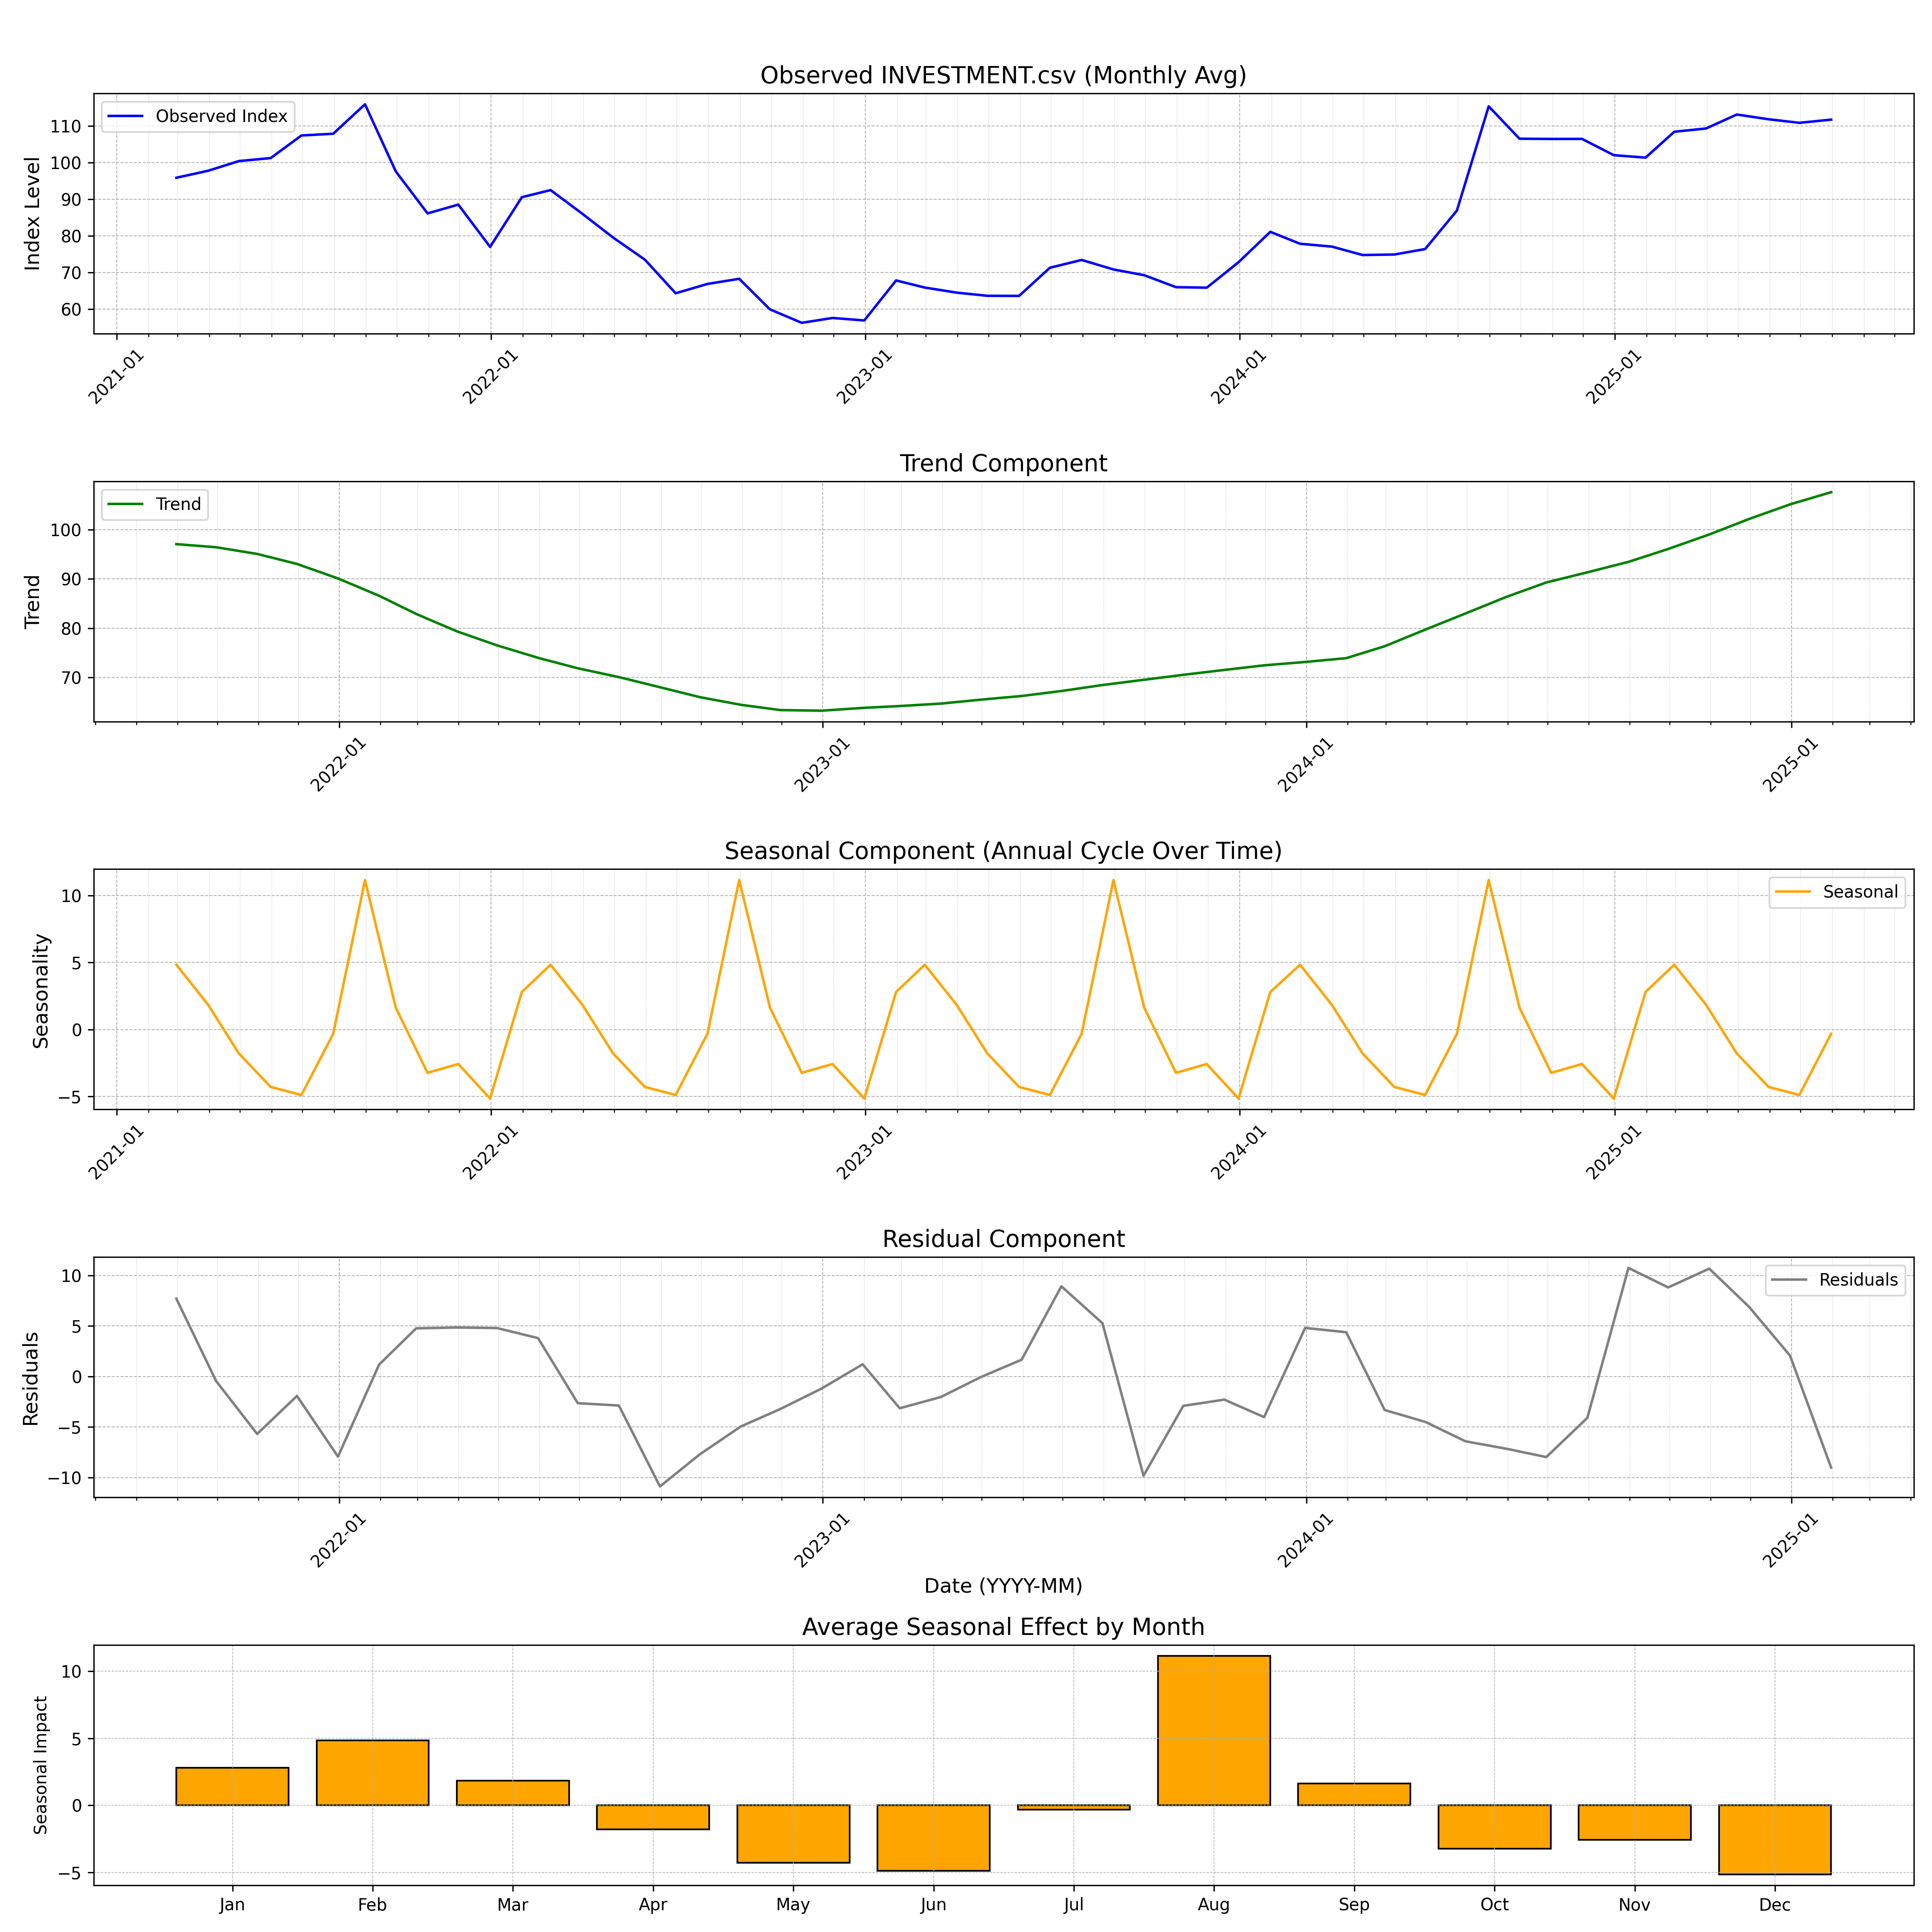
\includegraphics[width=0.9\textwidth]{decomposition_outputs/INVESTMENT_seasonal_decomposition.png}
    \caption{Seasonal Decomposition of INVESTMENT Index Monthly Returns}
\end{figure}

\begin{figure}[h!]
    \centering
    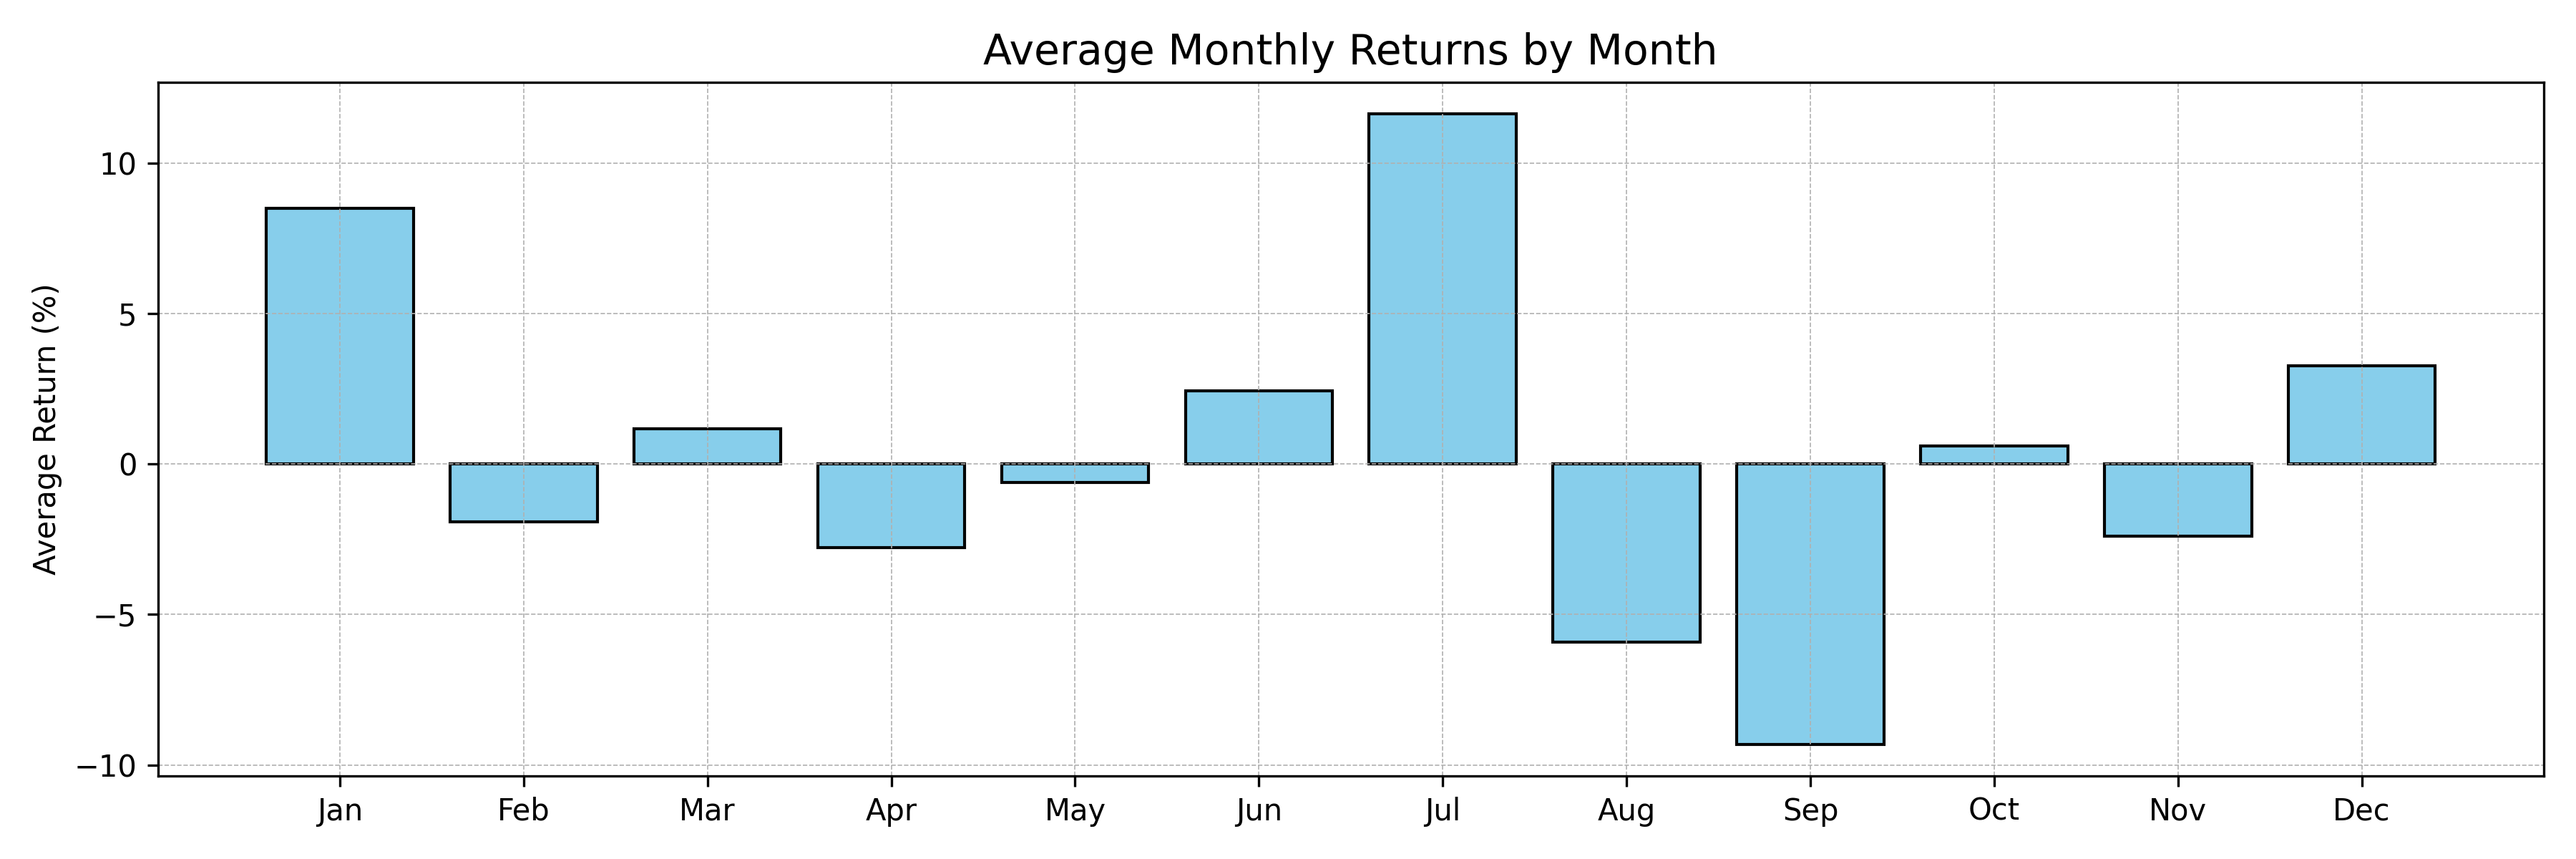
\includegraphics[width=0.7\textwidth]{decomposition_outputs/INVESTMENT_avg_monthly_returns.png}
    \caption{Average Monthly Returns by Month -- INVESTMENT}
\end{figure}

\begin{table}[h!]
\centering
\caption{Average Monthly Returns -- INVESTMENT}
\begin{tabular}{l r}
\toprule
Month & Value (\%) \\
\midrule
Jan & 8.49 \\
Feb & -1.93 \\
Mar & 1.16 \\
Apr & -2.78 \\
May & -0.61 \\
Jun & 2.43 \\
Jul & 11.63 \\
Aug & -5.92 \\
Sep & -9.31 \\
Oct & 0.60 \\
Nov & -2.39 \\
Dec & 3.25 \\
\bottomrule
\end{tabular}
\end{table}

\begin{table}[h!]
\centering
\caption{Average Seasonality -- INVESTMENT}
\begin{tabular}{l r}
\toprule
Month & Value (\%) \\
\midrule
Jan & 8.37 \\
Feb & -5.94 \\
Mar & 0.82 \\
Apr & -4.79 \\
May & -2.14 \\
Jun & 2.75 \\
Jul & 16.67 \\
Aug & -6.41 \\
Sep & -9.72 \\
Oct & 0.24 \\
Nov & -2.83 \\
Dec & 2.98 \\
\bottomrule
\end{tabular}
\end{table}


\clearpage

\subsection{LIFEINSU}
\textbf{Mean Monthly Return:} 1.23\% \\
\textbf{Median Monthly Return:} 0.17\% \\
\textbf{Standard Deviation:} 4.43\% \\
\textbf{Best Month:} Dec (9.06\%) \\
\textbf{Worst Month:} Sep (-3.70\%) \\
\textbf{Seasonal Amplitude:} 12.76\% \\
\textbf{August Return:} -3.17\% \\

\begin{figure}[h!]
    \centering
    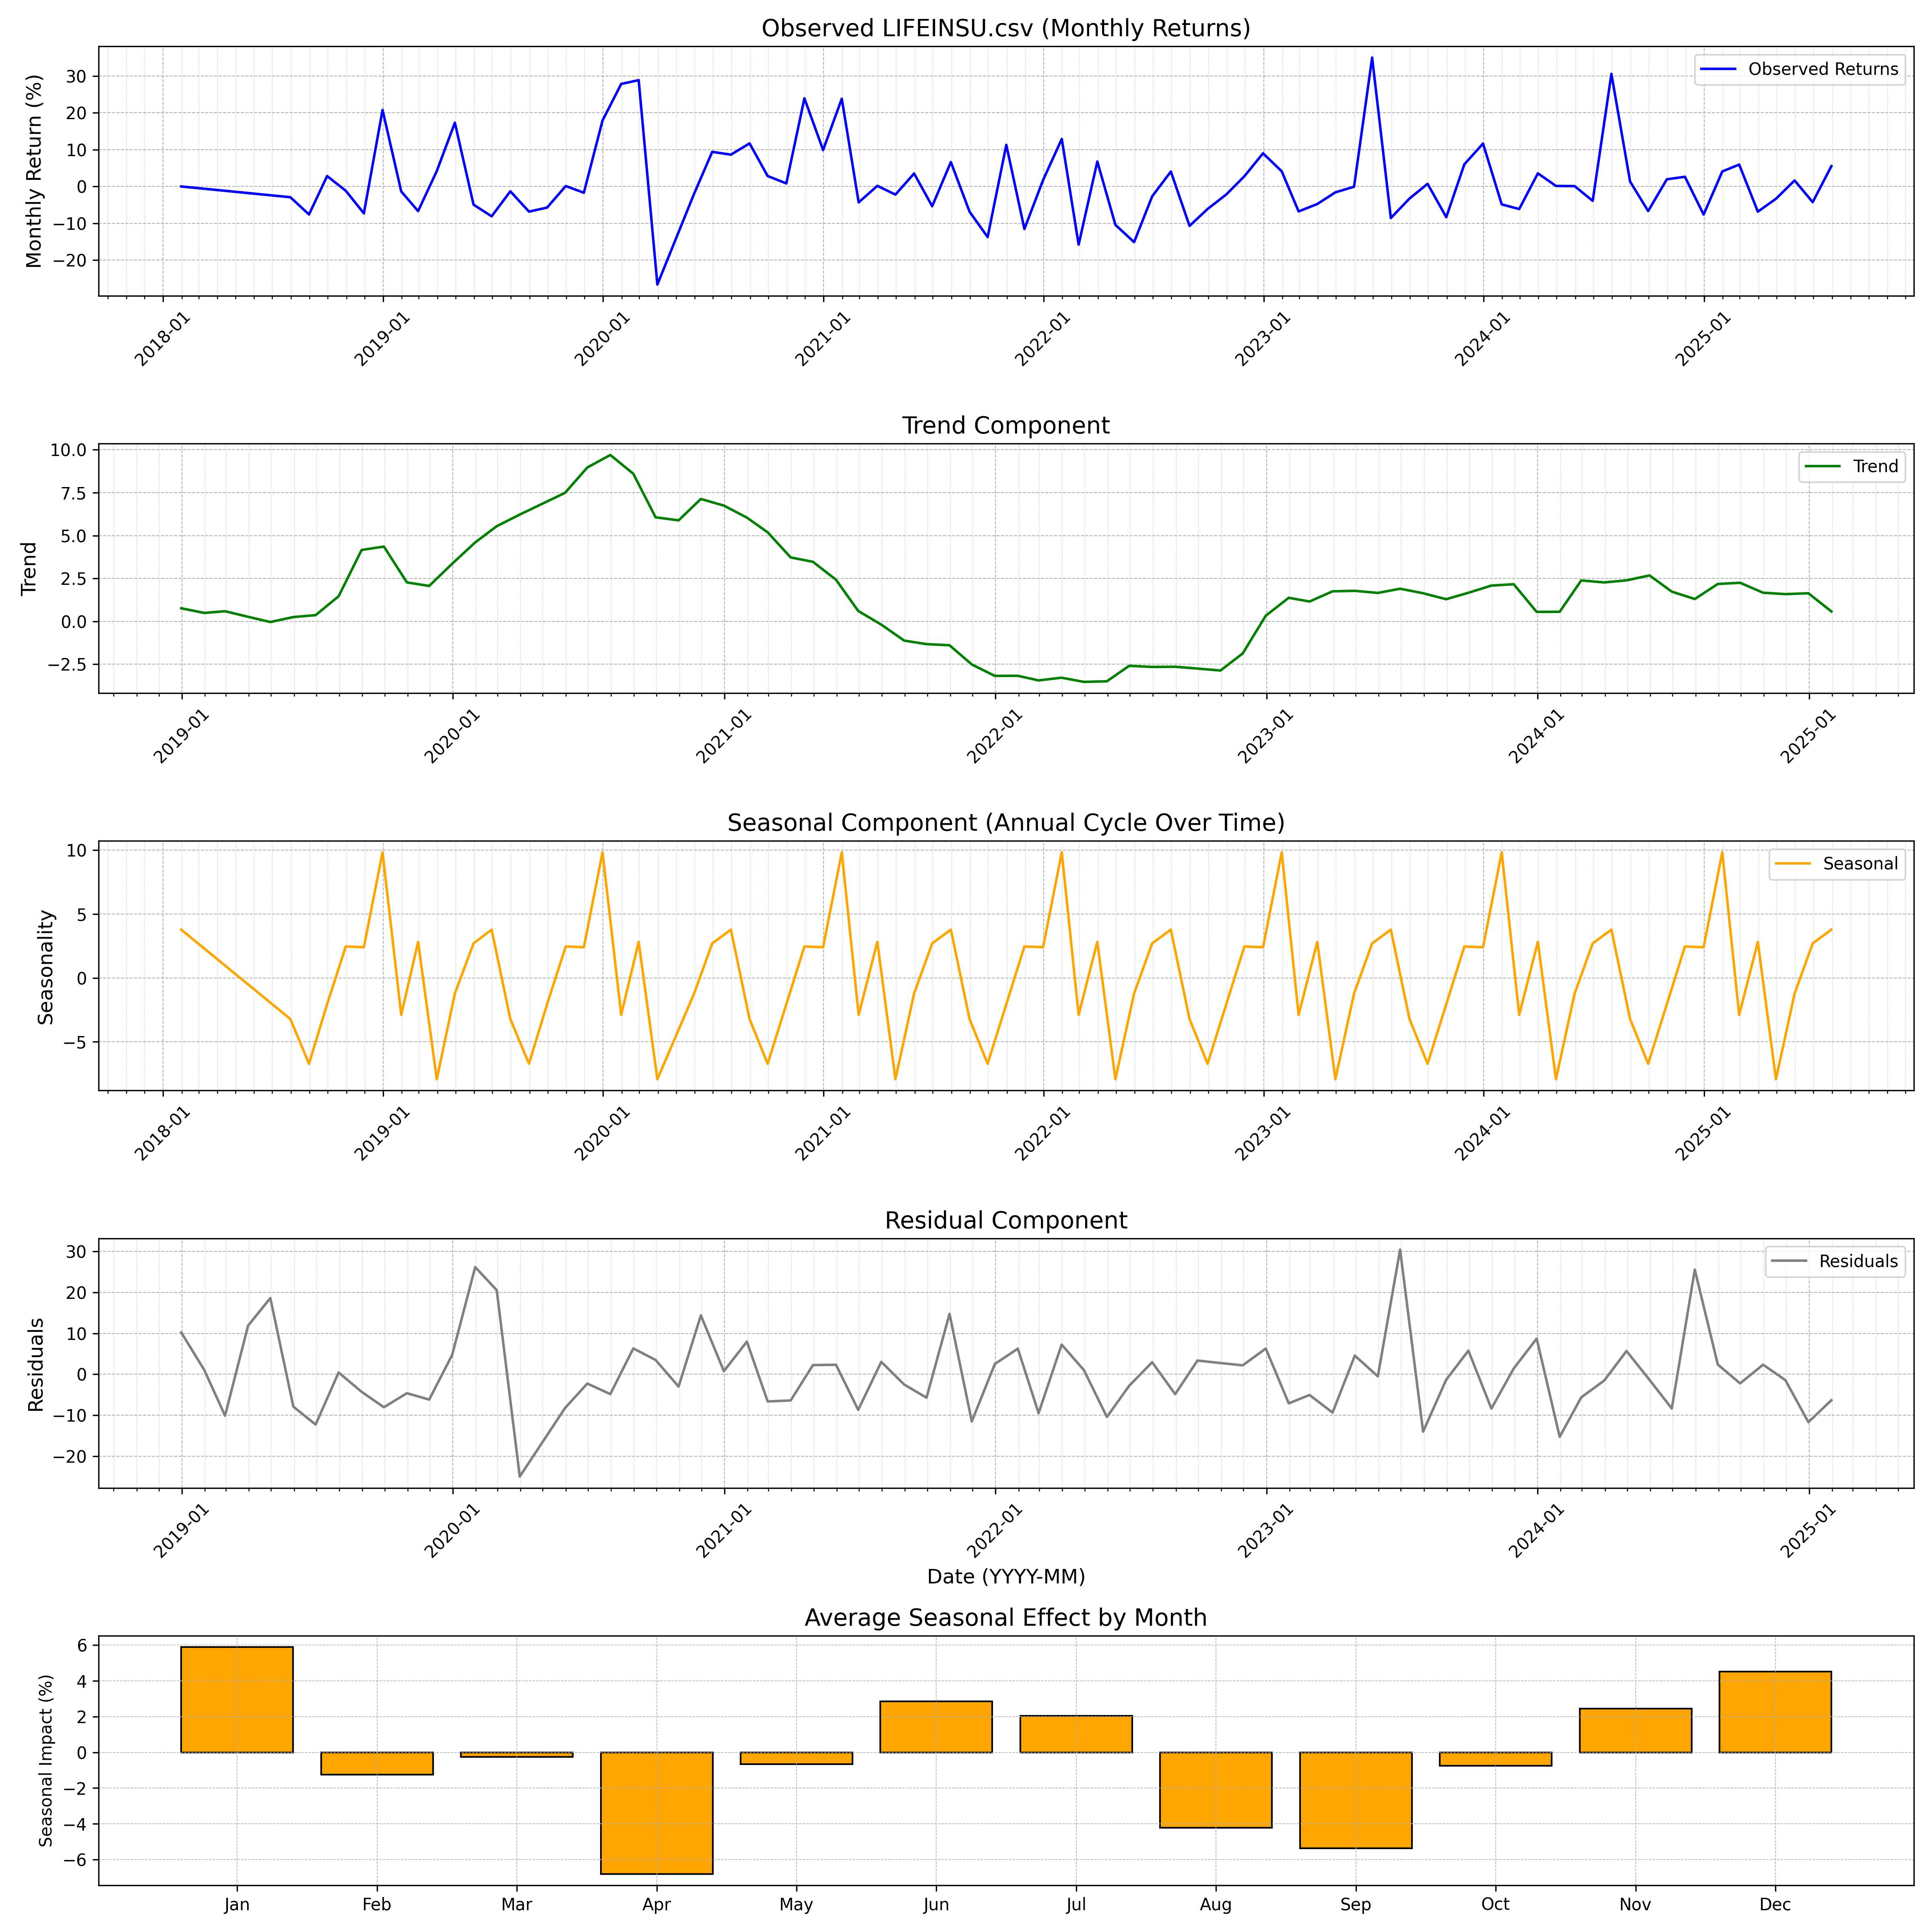
\includegraphics[width=0.9\textwidth]{decomposition_outputs/LIFEINSU_seasonal_decomposition.png}
    \caption{Seasonal Decomposition of LIFEINSU Index Monthly Returns}
\end{figure}

\begin{figure}[h!]
    \centering
    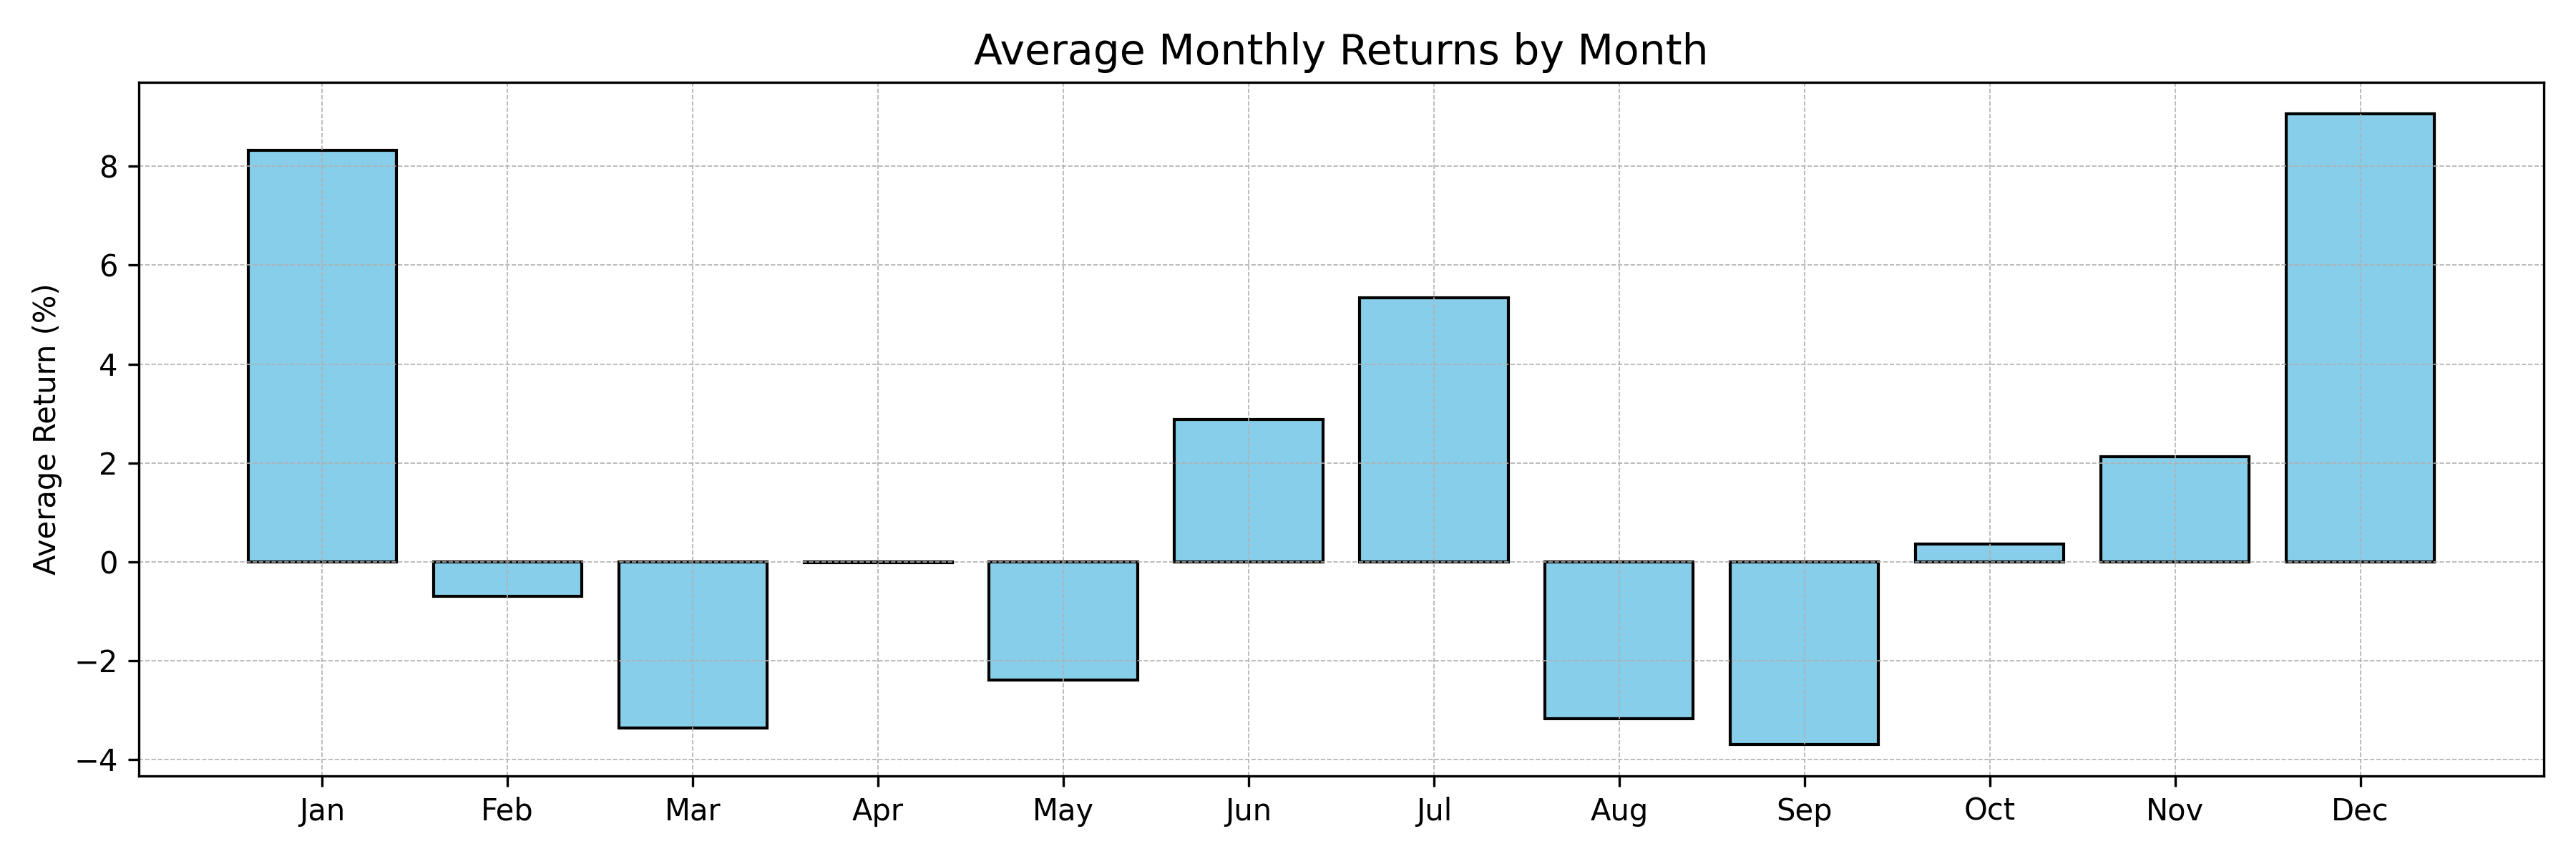
\includegraphics[width=0.7\textwidth]{decomposition_outputs/LIFEINSU_avg_monthly_returns.png}
    \caption{Average Monthly Returns by Month -- LIFEINSU}
\end{figure}

\begin{table}[h!]
\centering
\caption{Average Monthly Returns -- LIFEINSU}
\begin{tabular}{l r}
\toprule
Month & Value (\%) \\
\midrule
Jan & 8.33 \\
Feb & -0.70 \\
Mar & -3.36 \\
Apr & -0.01 \\
May & -2.40 \\
Jun & 2.87 \\
Jul & 5.33 \\
Aug & -3.17 \\
Sep & -3.70 \\
Oct & 0.36 \\
Nov & 2.12 \\
Dec & 9.06 \\
\bottomrule
\end{tabular}
\end{table}

\begin{table}[h!]
\centering
\caption{Average Seasonality -- LIFEINSU}
\begin{tabular}{l r}
\toprule
Month & Value (\%) \\
\midrule
Jan & 5.90 \\
Feb & -1.26 \\
Mar & -0.25 \\
Apr & -6.81 \\
May & -0.66 \\
Jun & 2.86 \\
Jul & 2.03 \\
Aug & -4.21 \\
Sep & -5.38 \\
Oct & -0.76 \\
Nov & 2.45 \\
Dec & 4.53 \\
\bottomrule
\end{tabular}
\end{table}


\clearpage

\subsection{MANUFACTURE}
\textbf{Mean Monthly Return:} 1.71\% \\
\textbf{Median Monthly Return:} 1.86\% \\
\textbf{Standard Deviation:} 2.52\% \\
\textbf{Best Month:} Jul (5.72\%) \\
\textbf{Worst Month:} Mar (-2.69\%) \\
\textbf{Seasonal Amplitude:} 8.41\% \\
\textbf{August Return:} 0.49\% \\

\begin{figure}[h!]
    \centering
    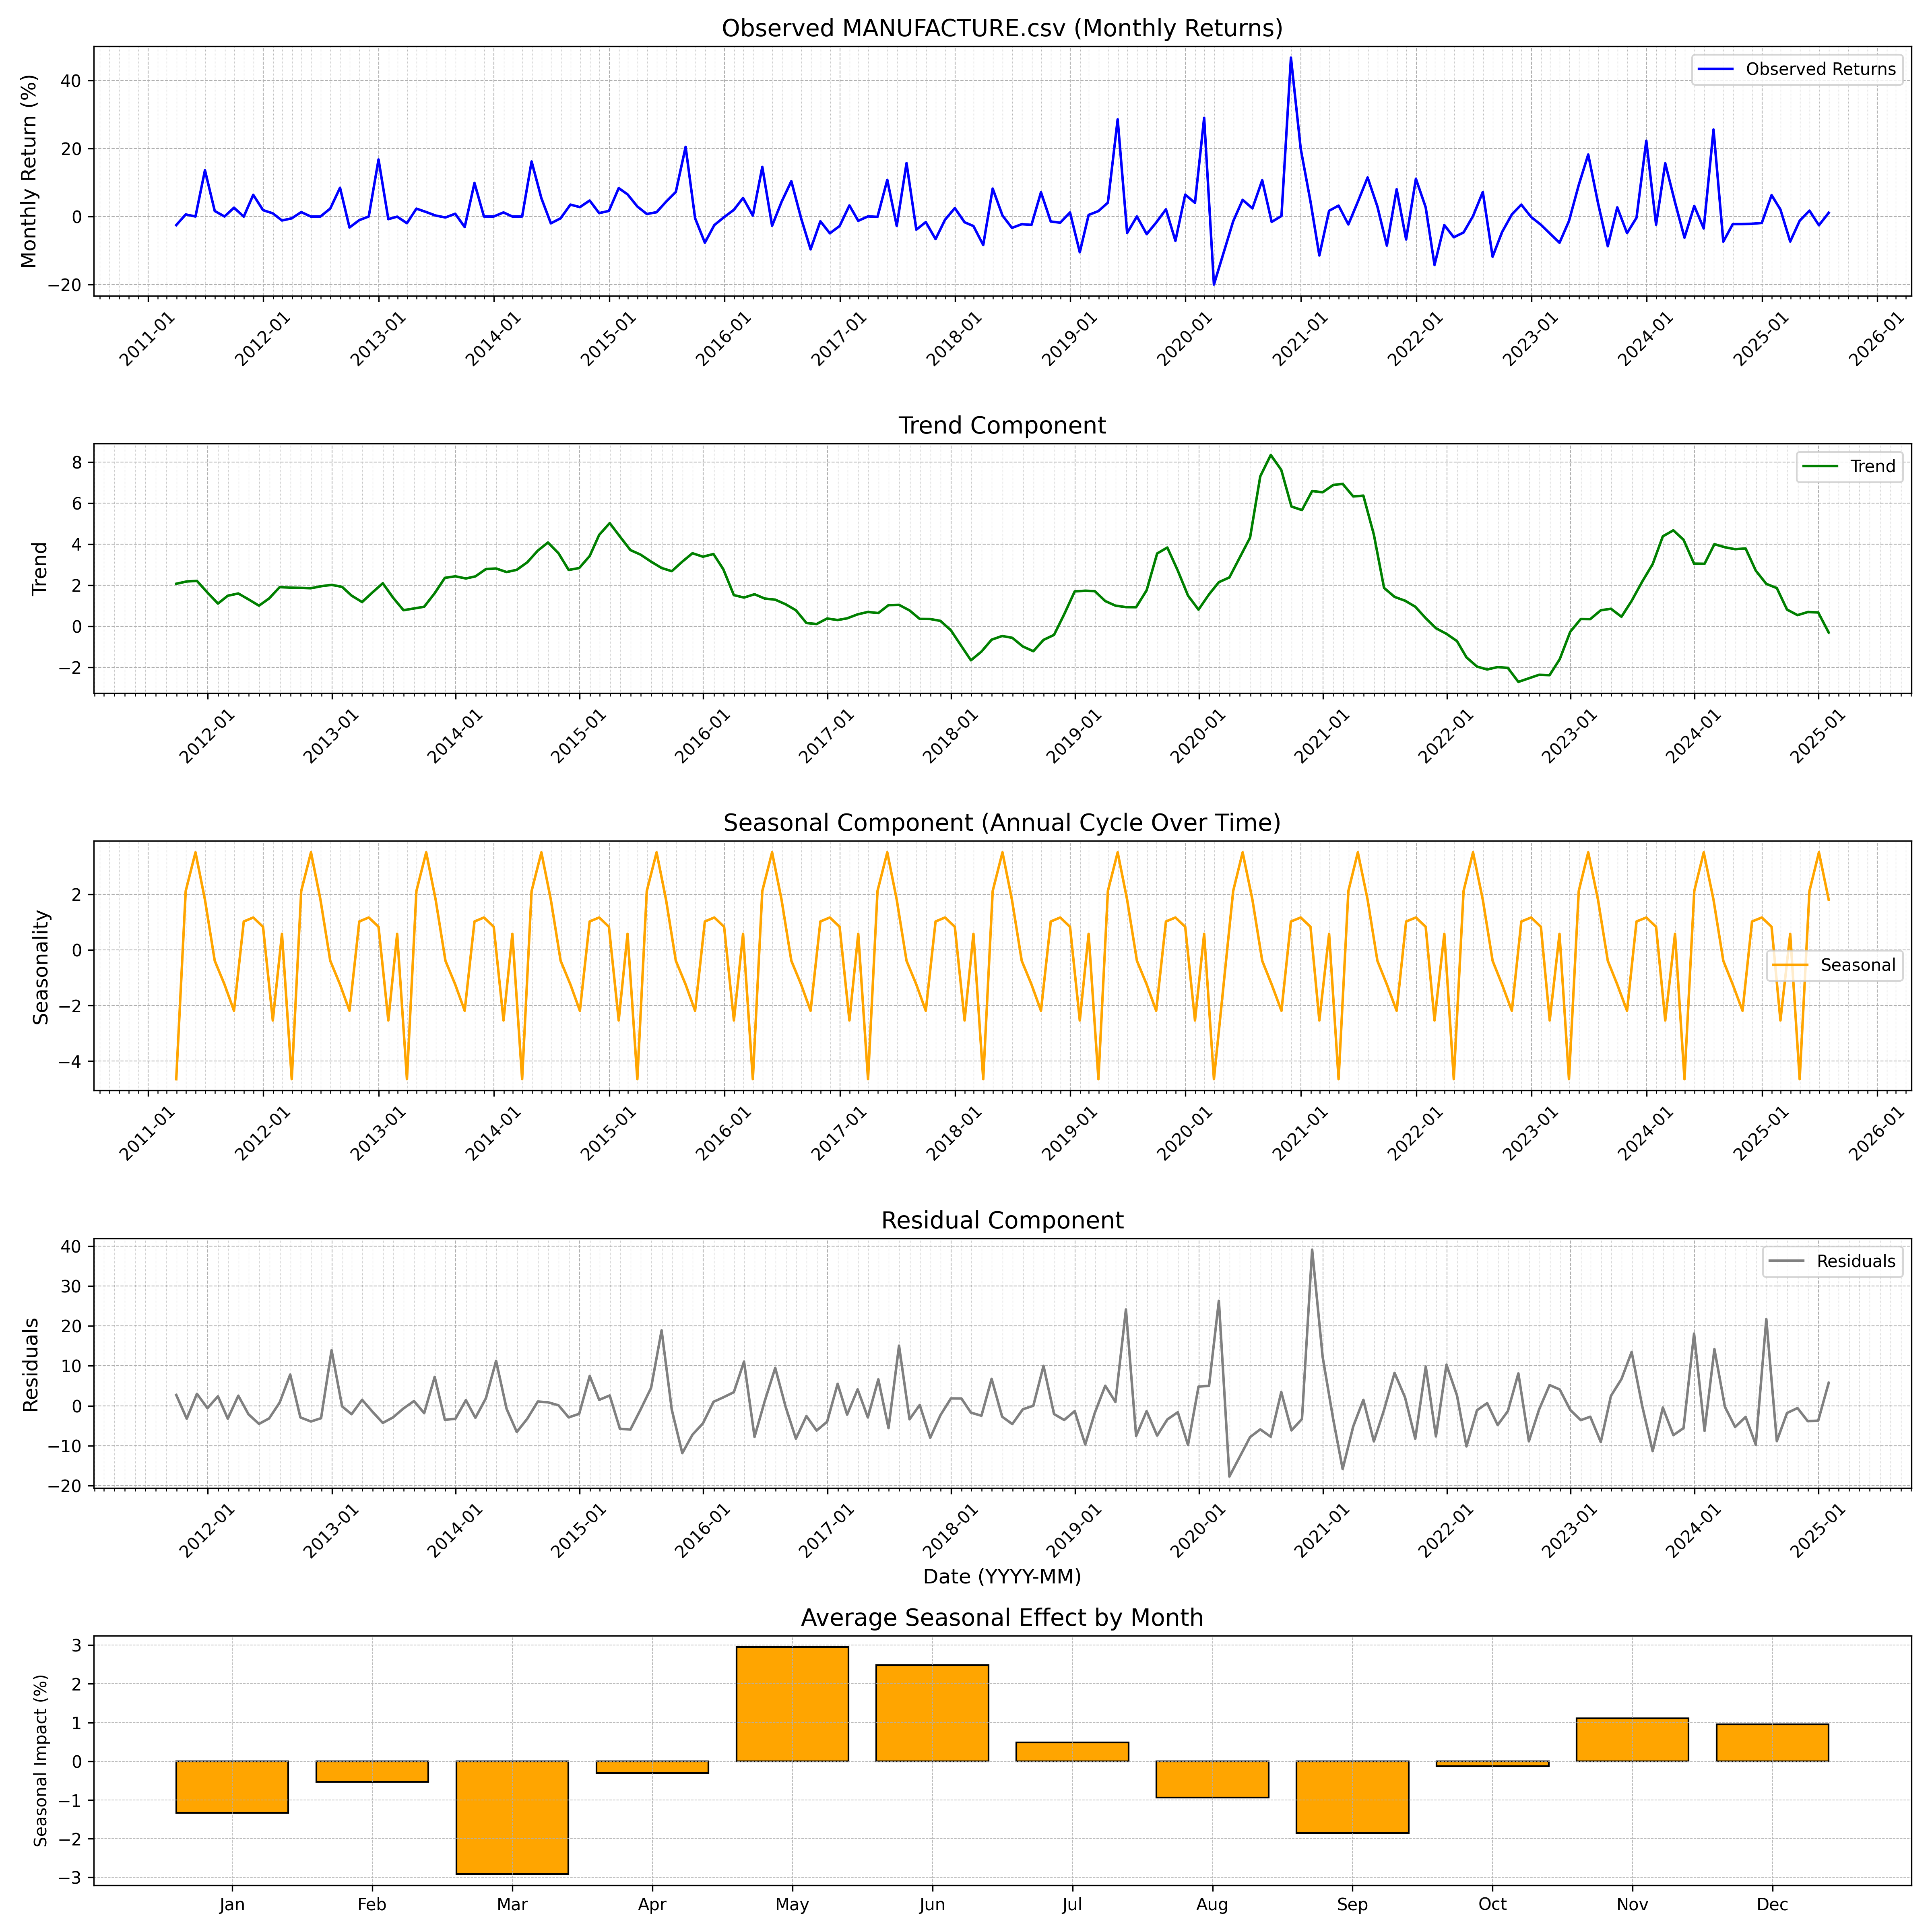
\includegraphics[width=0.9\textwidth]{decomposition_outputs/MANUFACTURE_seasonal_decomposition.png}
    \caption{Seasonal Decomposition of MANUFACTURE Index Monthly Returns}
\end{figure}

\begin{figure}[h!]
    \centering
    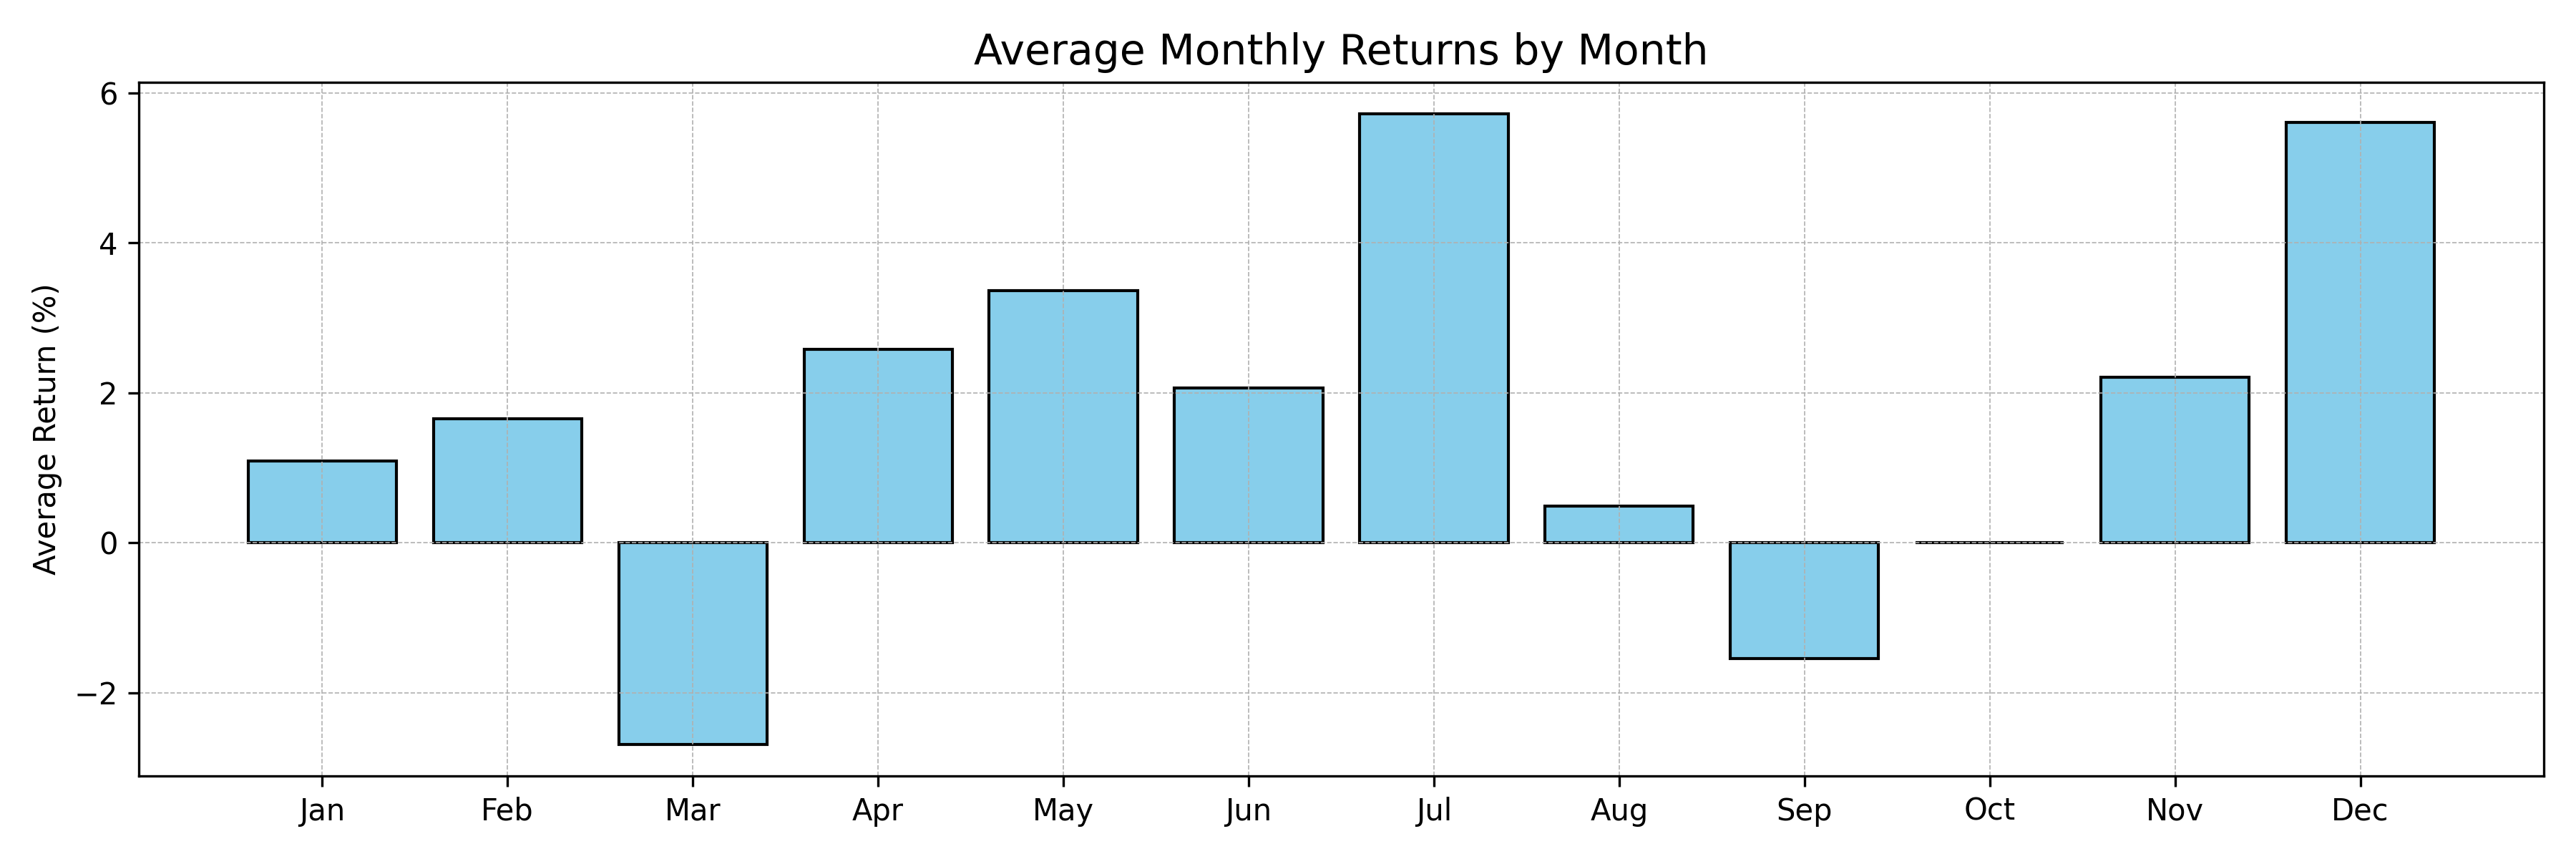
\includegraphics[width=0.7\textwidth]{decomposition_outputs/MANUFACTURE_avg_monthly_returns.png}
    \caption{Average Monthly Returns by Month -- MANUFACTURE}
\end{figure}

\begin{table}[h!]
\centering
\caption{Average Monthly Returns -- MANUFACTURE}
\begin{tabular}{l r}
\toprule
Month & Value (\%) \\
\midrule
Jan & 1.09 \\
Feb & 1.66 \\
Mar & -2.69 \\
Apr & 2.58 \\
May & 3.36 \\
Jun & 2.07 \\
Jul & 5.72 \\
Aug & 0.49 \\
Sep & -1.55 \\
Oct & -0.00 \\
Nov & 2.21 \\
Dec & 5.61 \\
\bottomrule
\end{tabular}
\end{table}

\begin{table}[h!]
\centering
\caption{Average Seasonality -- MANUFACTURE}
\begin{tabular}{l r}
\toprule
Month & Value (\%) \\
\midrule
Jan & -1.34 \\
Feb & -0.54 \\
Mar & -2.91 \\
Apr & -0.30 \\
May & 2.95 \\
Jun & 2.49 \\
Jul & 0.49 \\
Aug & -0.94 \\
Sep & -1.85 \\
Oct & -0.13 \\
Nov & 1.11 \\
Dec & 0.95 \\
\bottomrule
\end{tabular}
\end{table}


\clearpage

\subsection{MICROFINANCE}
\textbf{Mean Monthly Return:} 1.75\% \\
\textbf{Median Monthly Return:} 0.62\% \\
\textbf{Standard Deviation:} 4.80\% \\
\textbf{Best Month:} Jan (11.78\%) \\
\textbf{Worst Month:} Mar (-3.46\%) \\
\textbf{Seasonal Amplitude:} 15.24\% \\
\textbf{August Return:} -3.46\% \\

\begin{figure}[h!]
    \centering
    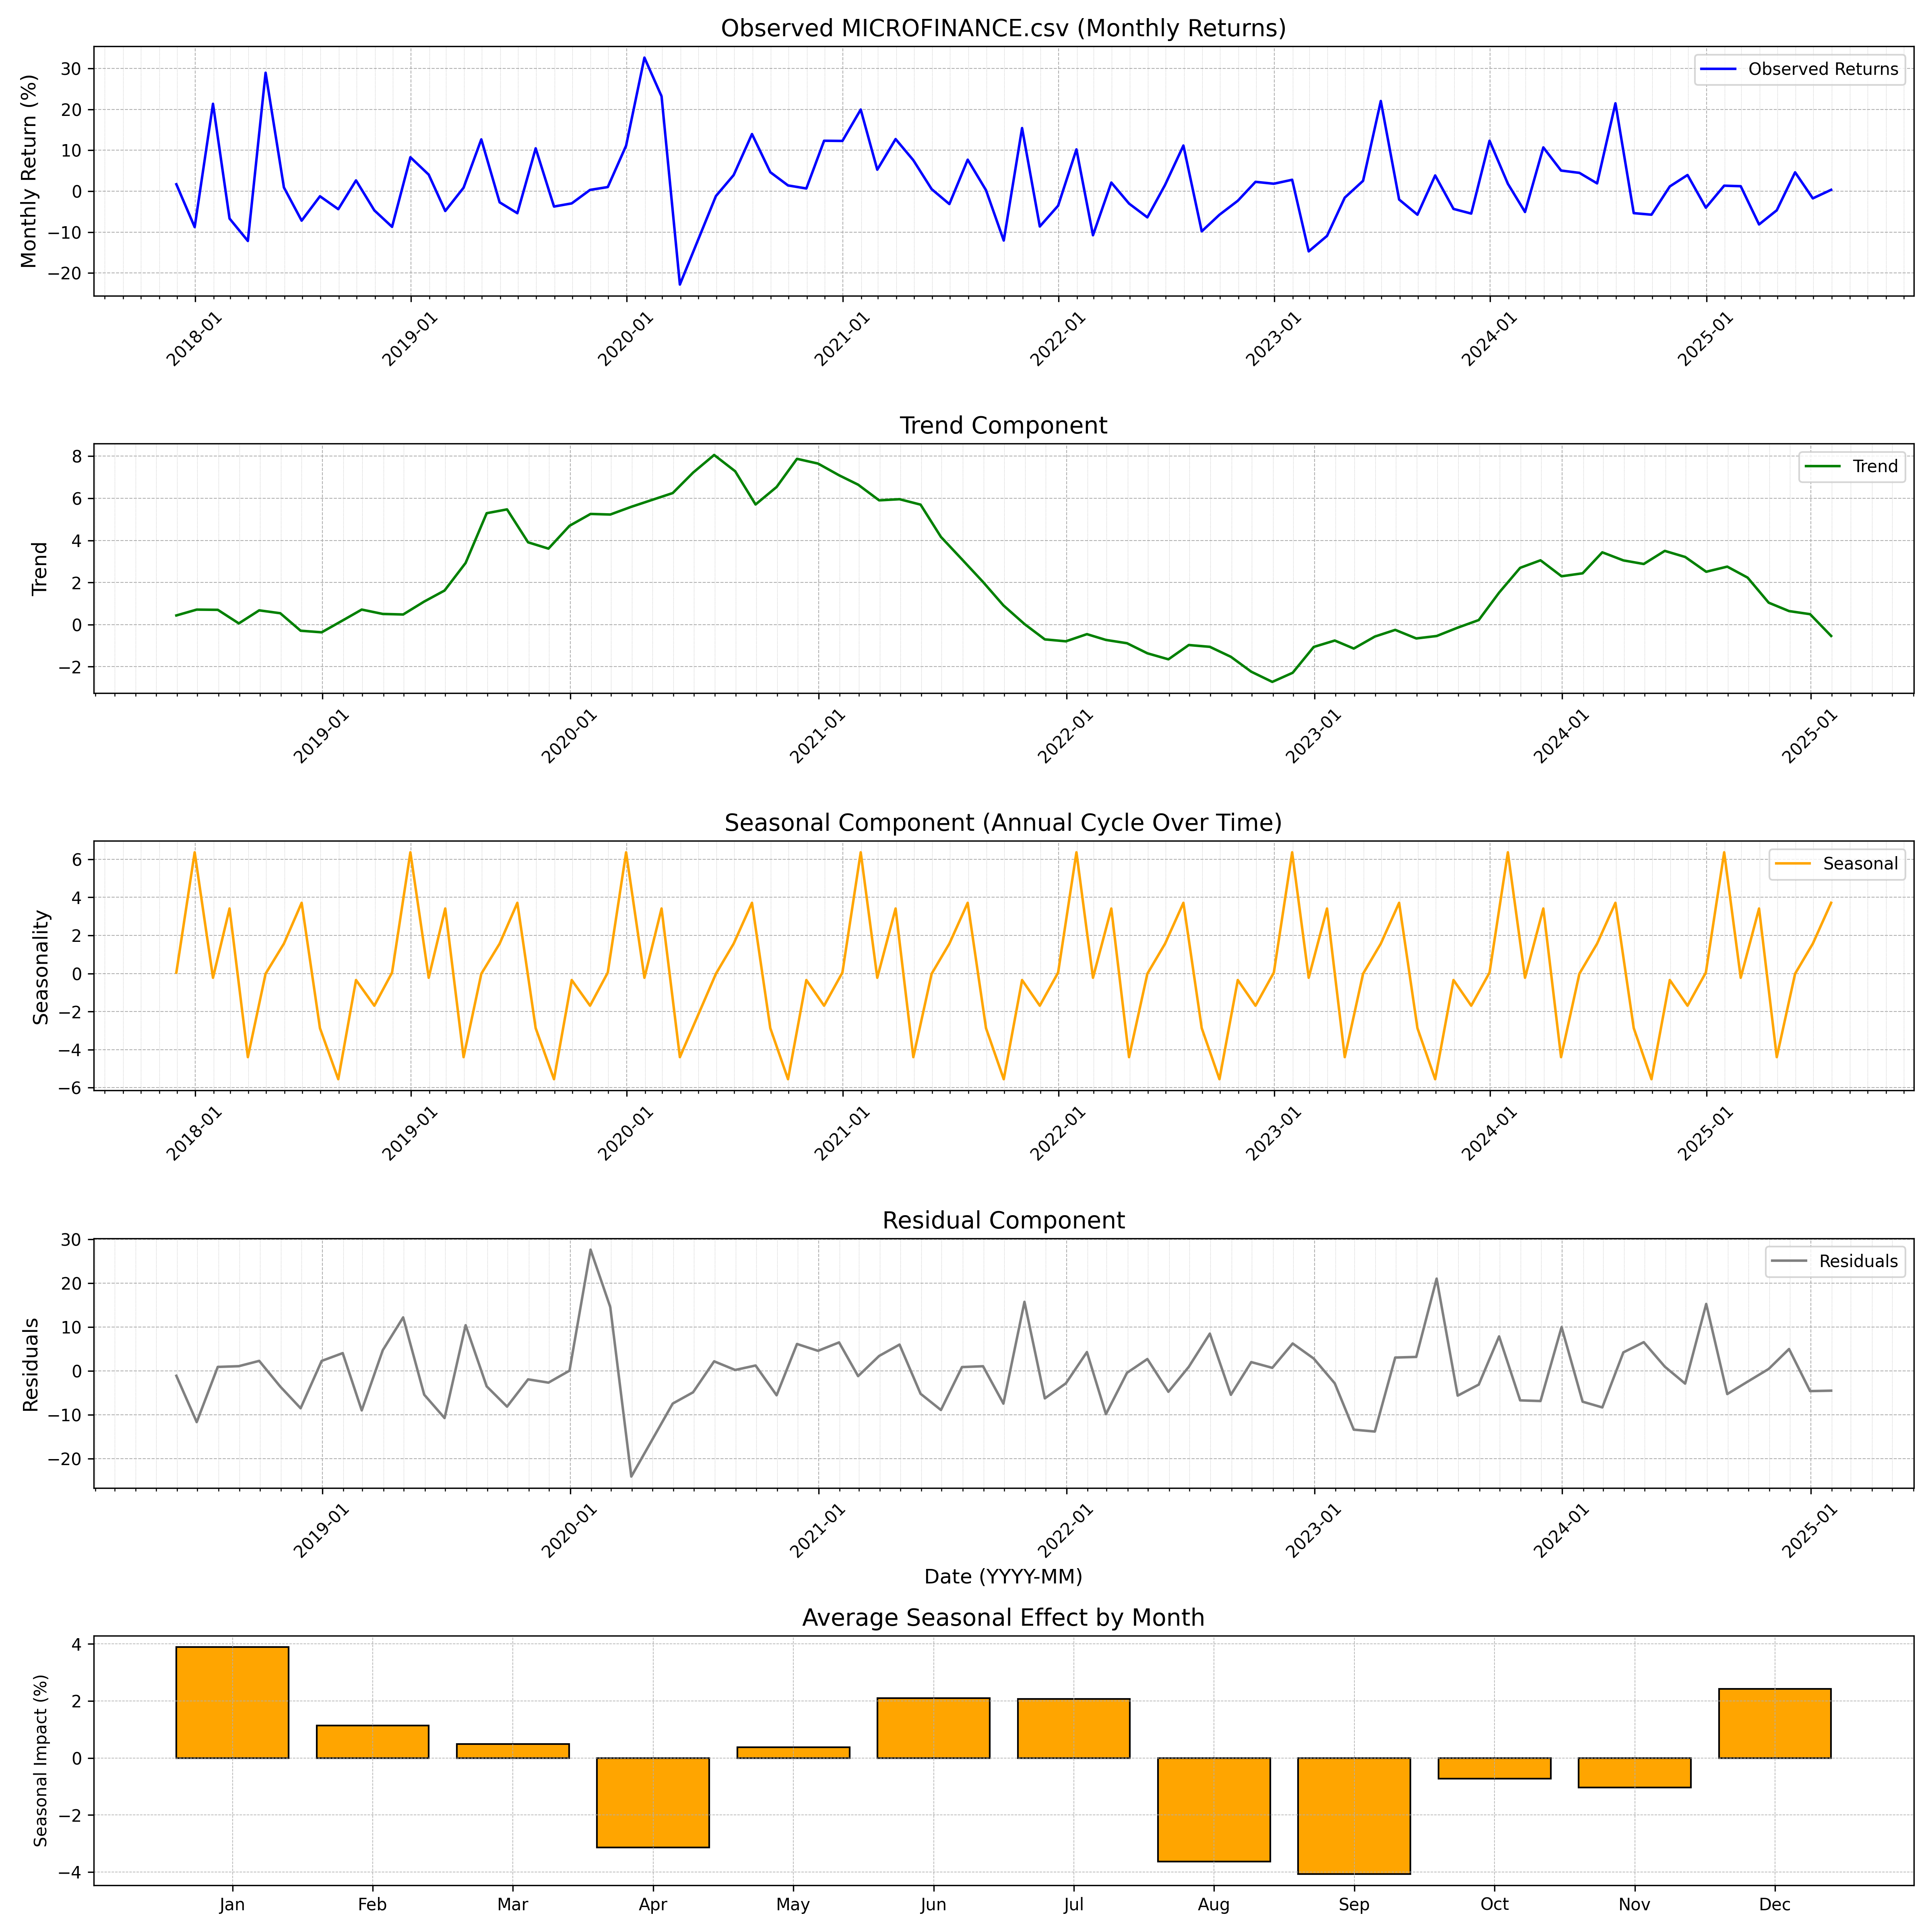
\includegraphics[width=0.9\textwidth]{decomposition_outputs/MICROFINANCE_seasonal_decomposition.png}
    \caption{Seasonal Decomposition of MICROFINANCE Index Monthly Returns}
\end{figure}

\begin{figure}[h!]
    \centering
    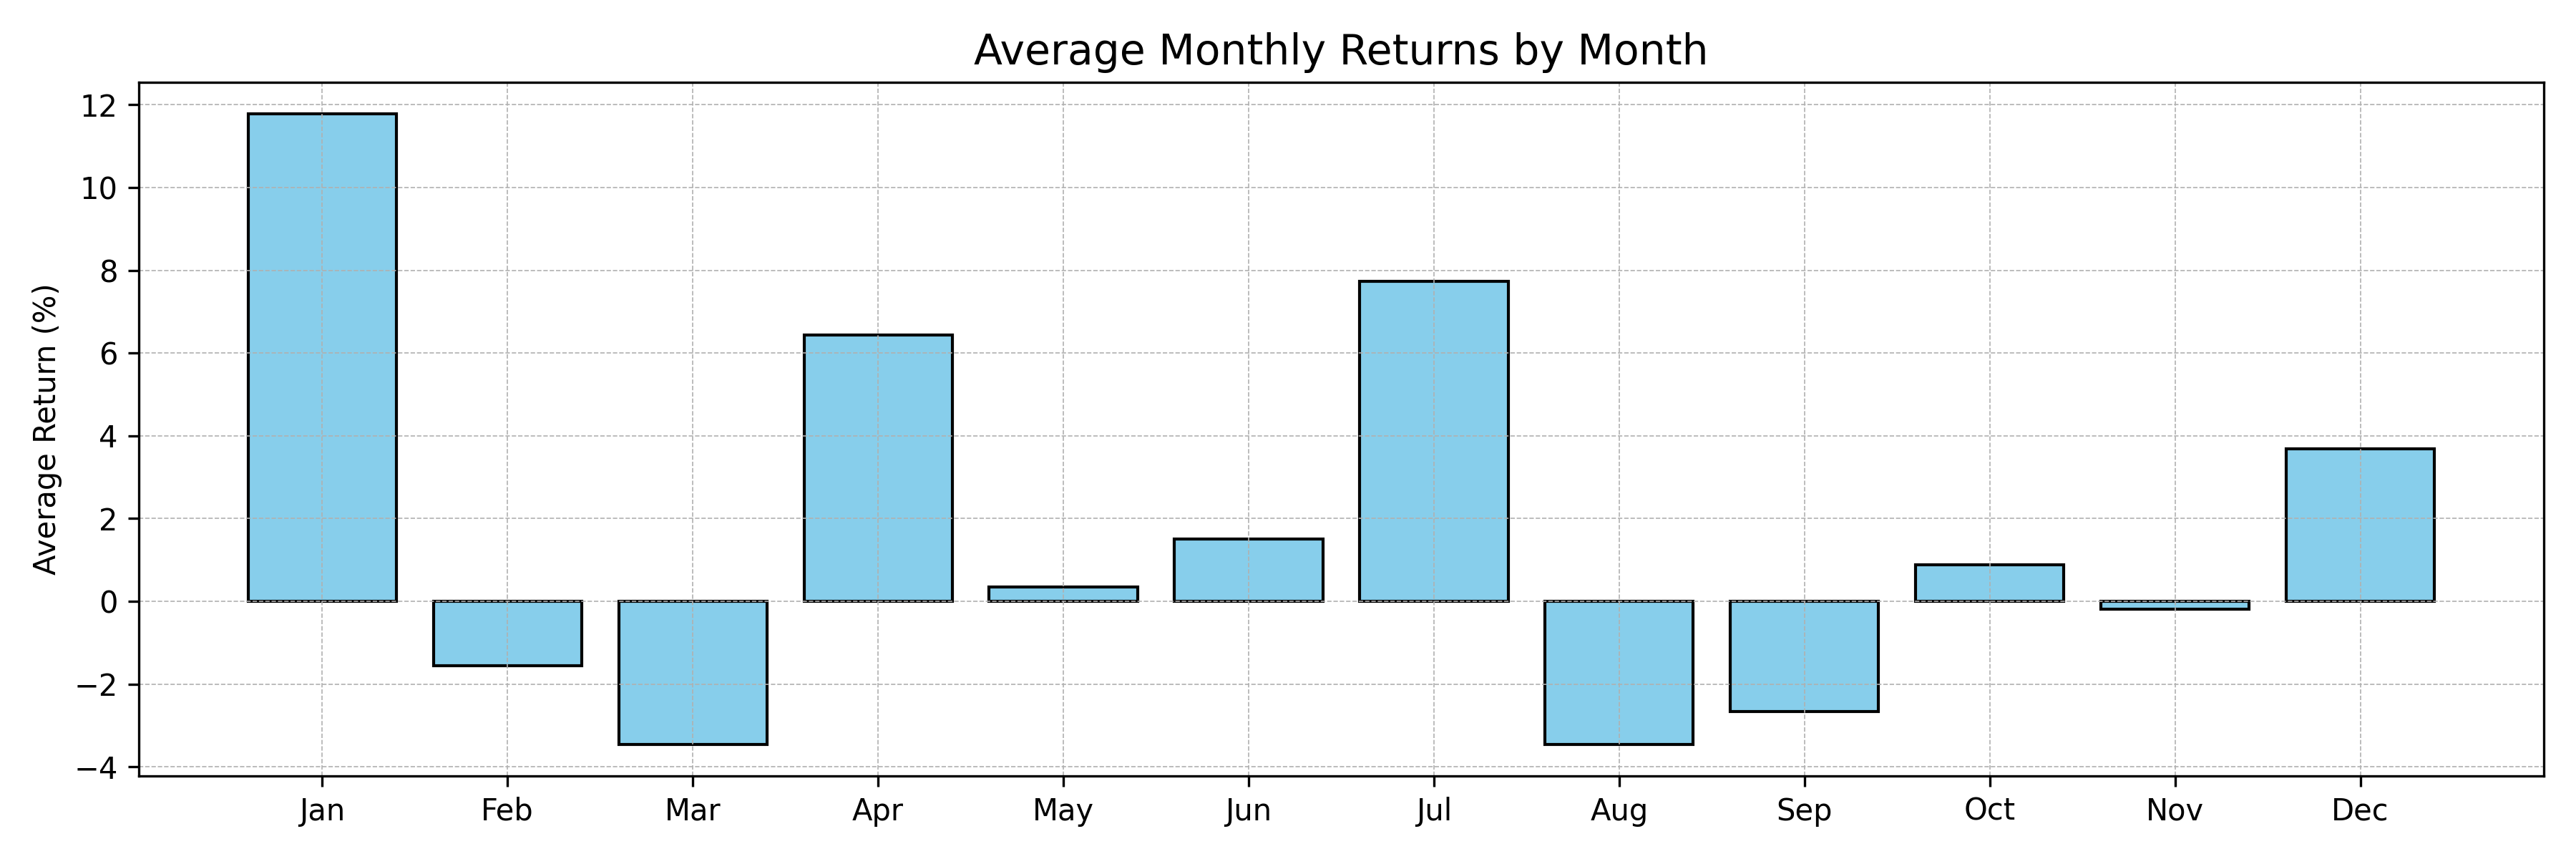
\includegraphics[width=0.7\textwidth]{decomposition_outputs/MICROFINANCE_avg_monthly_returns.png}
    \caption{Average Monthly Returns by Month -- MICROFINANCE}
\end{figure}

\begin{table}[h!]
\centering
\caption{Average Monthly Returns -- MICROFINANCE}
\begin{tabular}{l r}
\toprule
Month & Value (\%) \\
\midrule
Jan & 11.78 \\
Feb & -1.55 \\
Mar & -3.46 \\
Apr & 6.43 \\
May & 0.35 \\
Jun & 1.50 \\
Jul & 7.74 \\
Aug & -3.46 \\
Sep & -2.67 \\
Oct & 0.89 \\
Nov & -0.19 \\
Dec & 3.69 \\
\bottomrule
\end{tabular}
\end{table}

\begin{table}[h!]
\centering
\caption{Average Seasonality -- MICROFINANCE}
\begin{tabular}{l r}
\toprule
Month & Value (\%) \\
\midrule
Jan & 3.89 \\
Feb & 1.14 \\
Mar & 0.48 \\
Apr & -3.14 \\
May & 0.38 \\
Jun & 2.10 \\
Jul & 2.06 \\
Aug & -3.64 \\
Sep & -4.07 \\
Oct & -0.73 \\
Nov & -1.04 \\
Dec & 2.42 \\
\bottomrule
\end{tabular}
\end{table}


\clearpage

\subsection{NONLIFEINSU}
\textbf{Mean Monthly Return:} 1.24\% \\
\textbf{Median Monthly Return:} 0.06\% \\
\textbf{Standard Deviation:} 4.20\% \\
\textbf{Best Month:} Jan (10.10\%) \\
\textbf{Worst Month:} Sep (-3.55\%) \\
\textbf{Seasonal Amplitude:} 13.65\% \\
\textbf{August Return:} -1.77\% \\

\begin{figure}[h!]
    \centering
    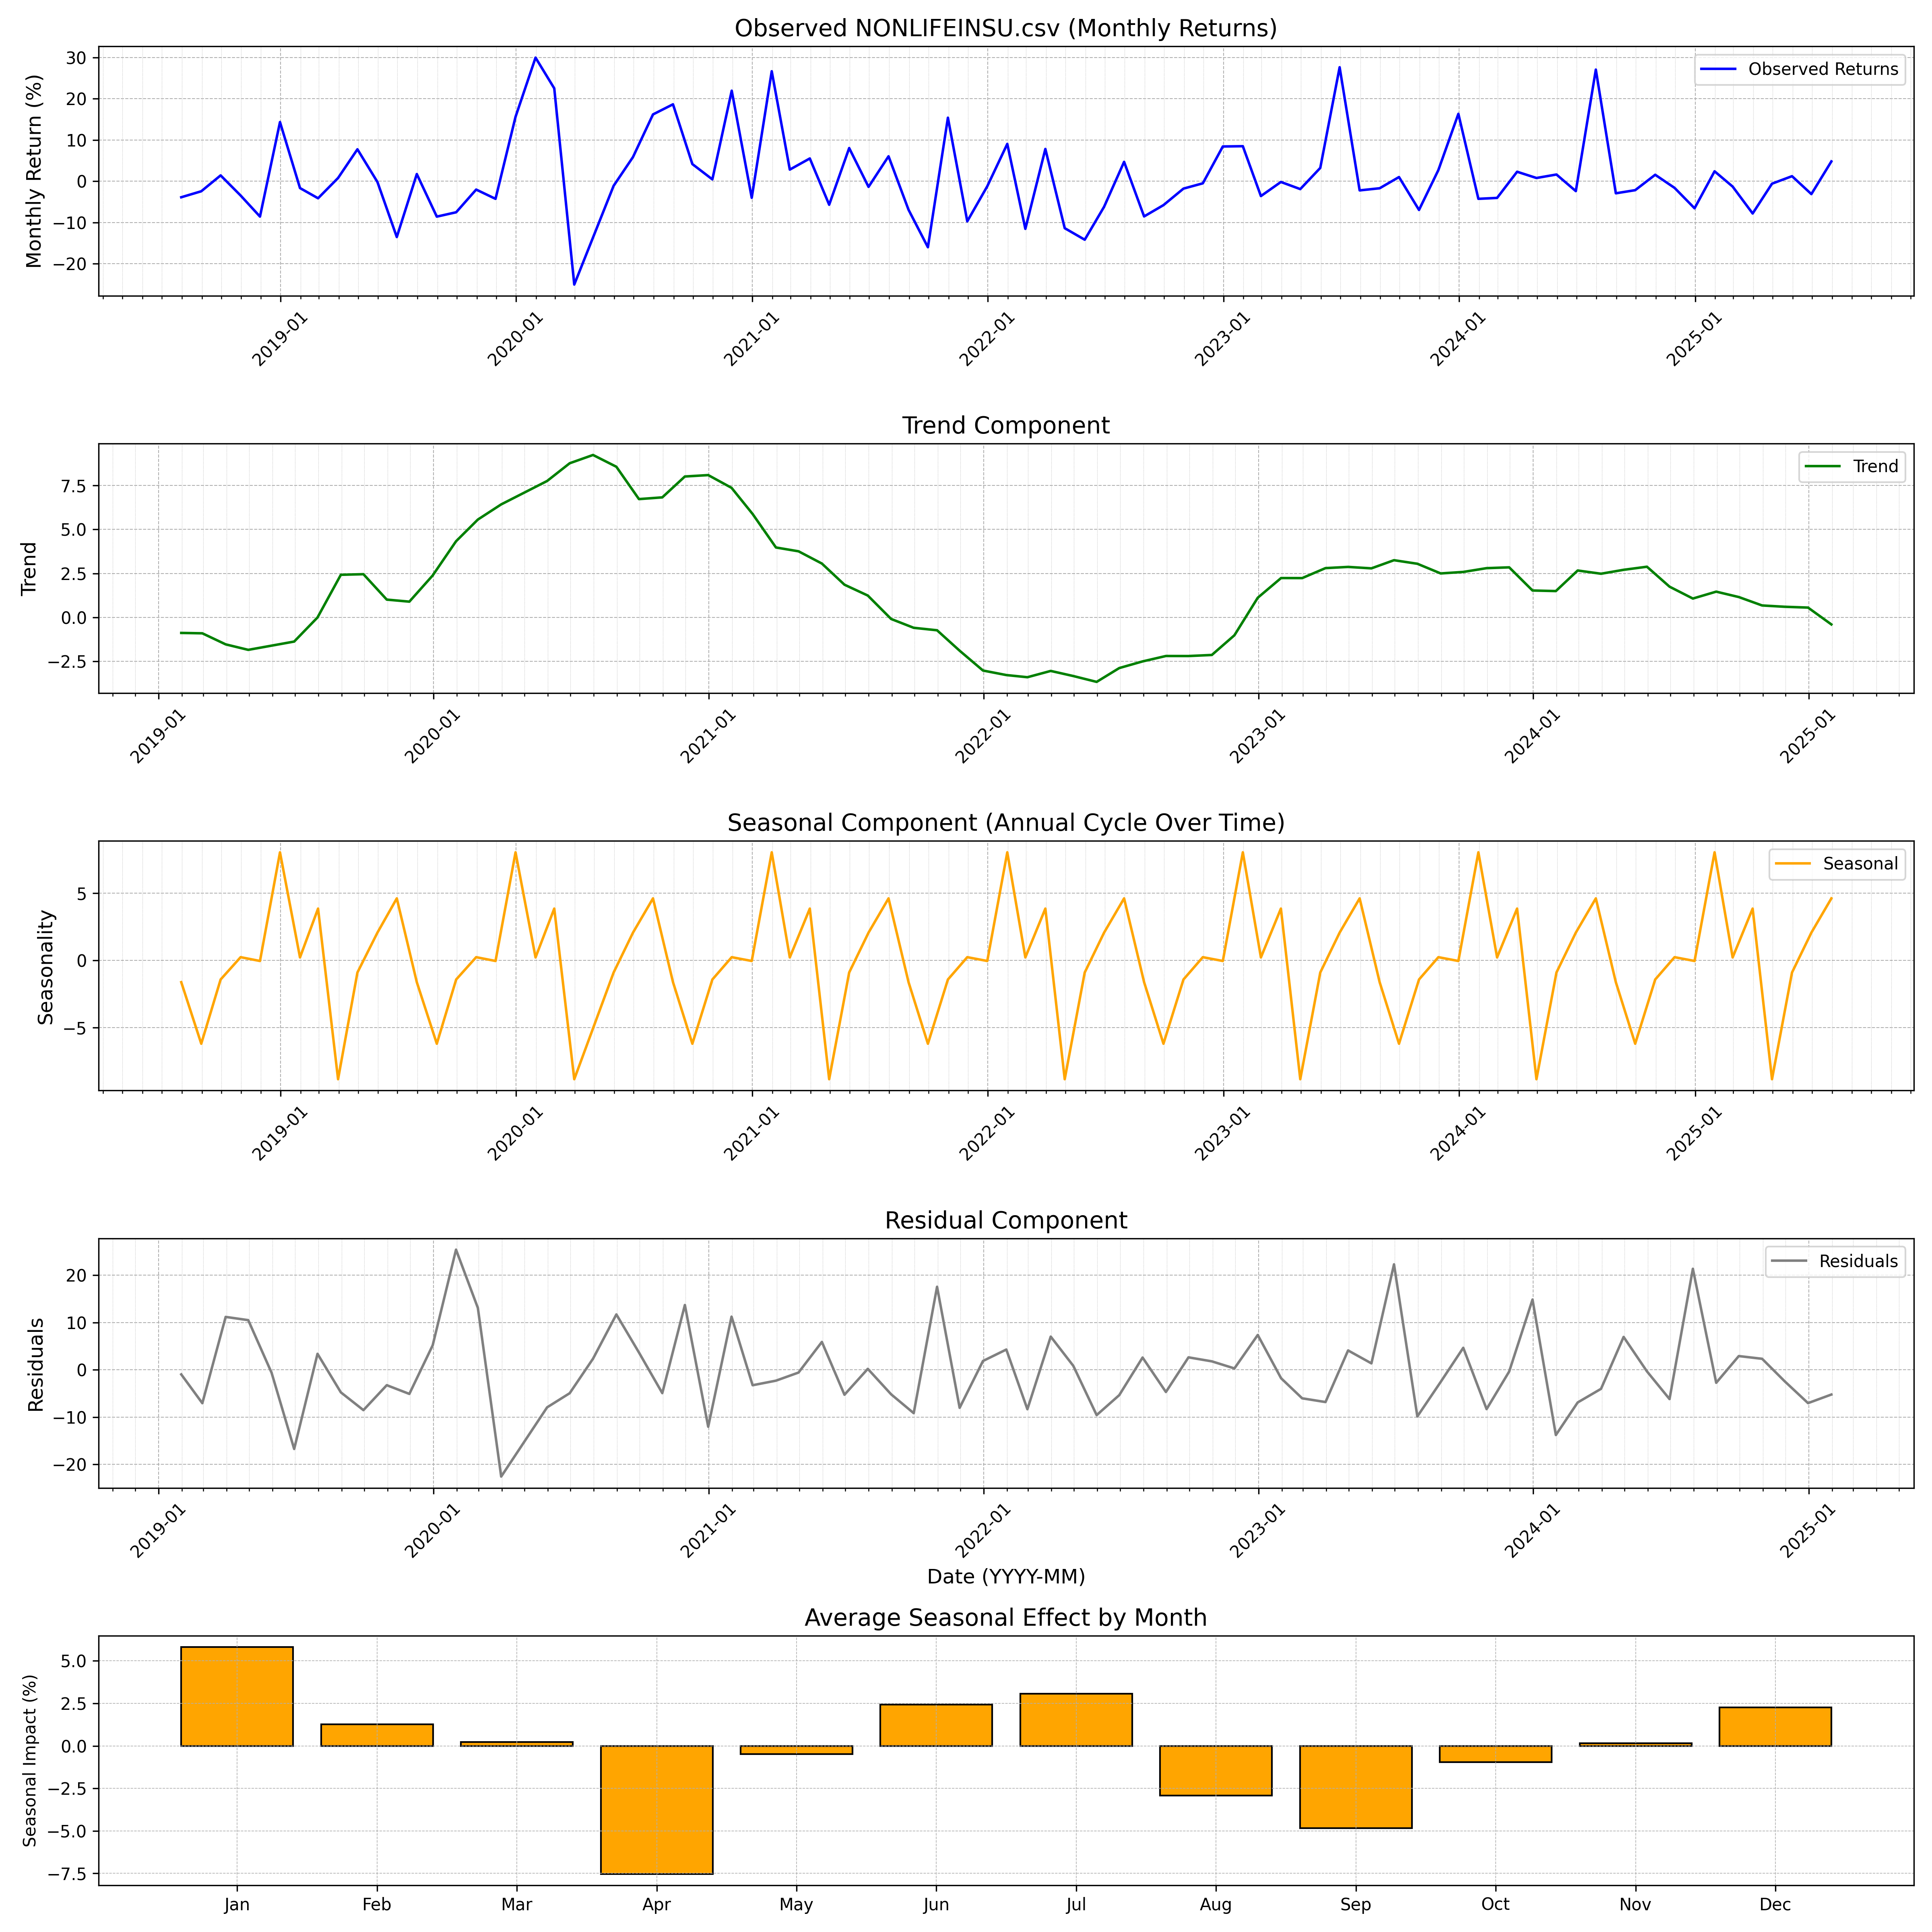
\includegraphics[width=0.9\textwidth]{decomposition_outputs/NONLIFEINSU_seasonal_decomposition.png}
    \caption{Seasonal Decomposition of NONLIFEINSU Index Monthly Returns}
\end{figure}

\begin{figure}[h!]
    \centering
    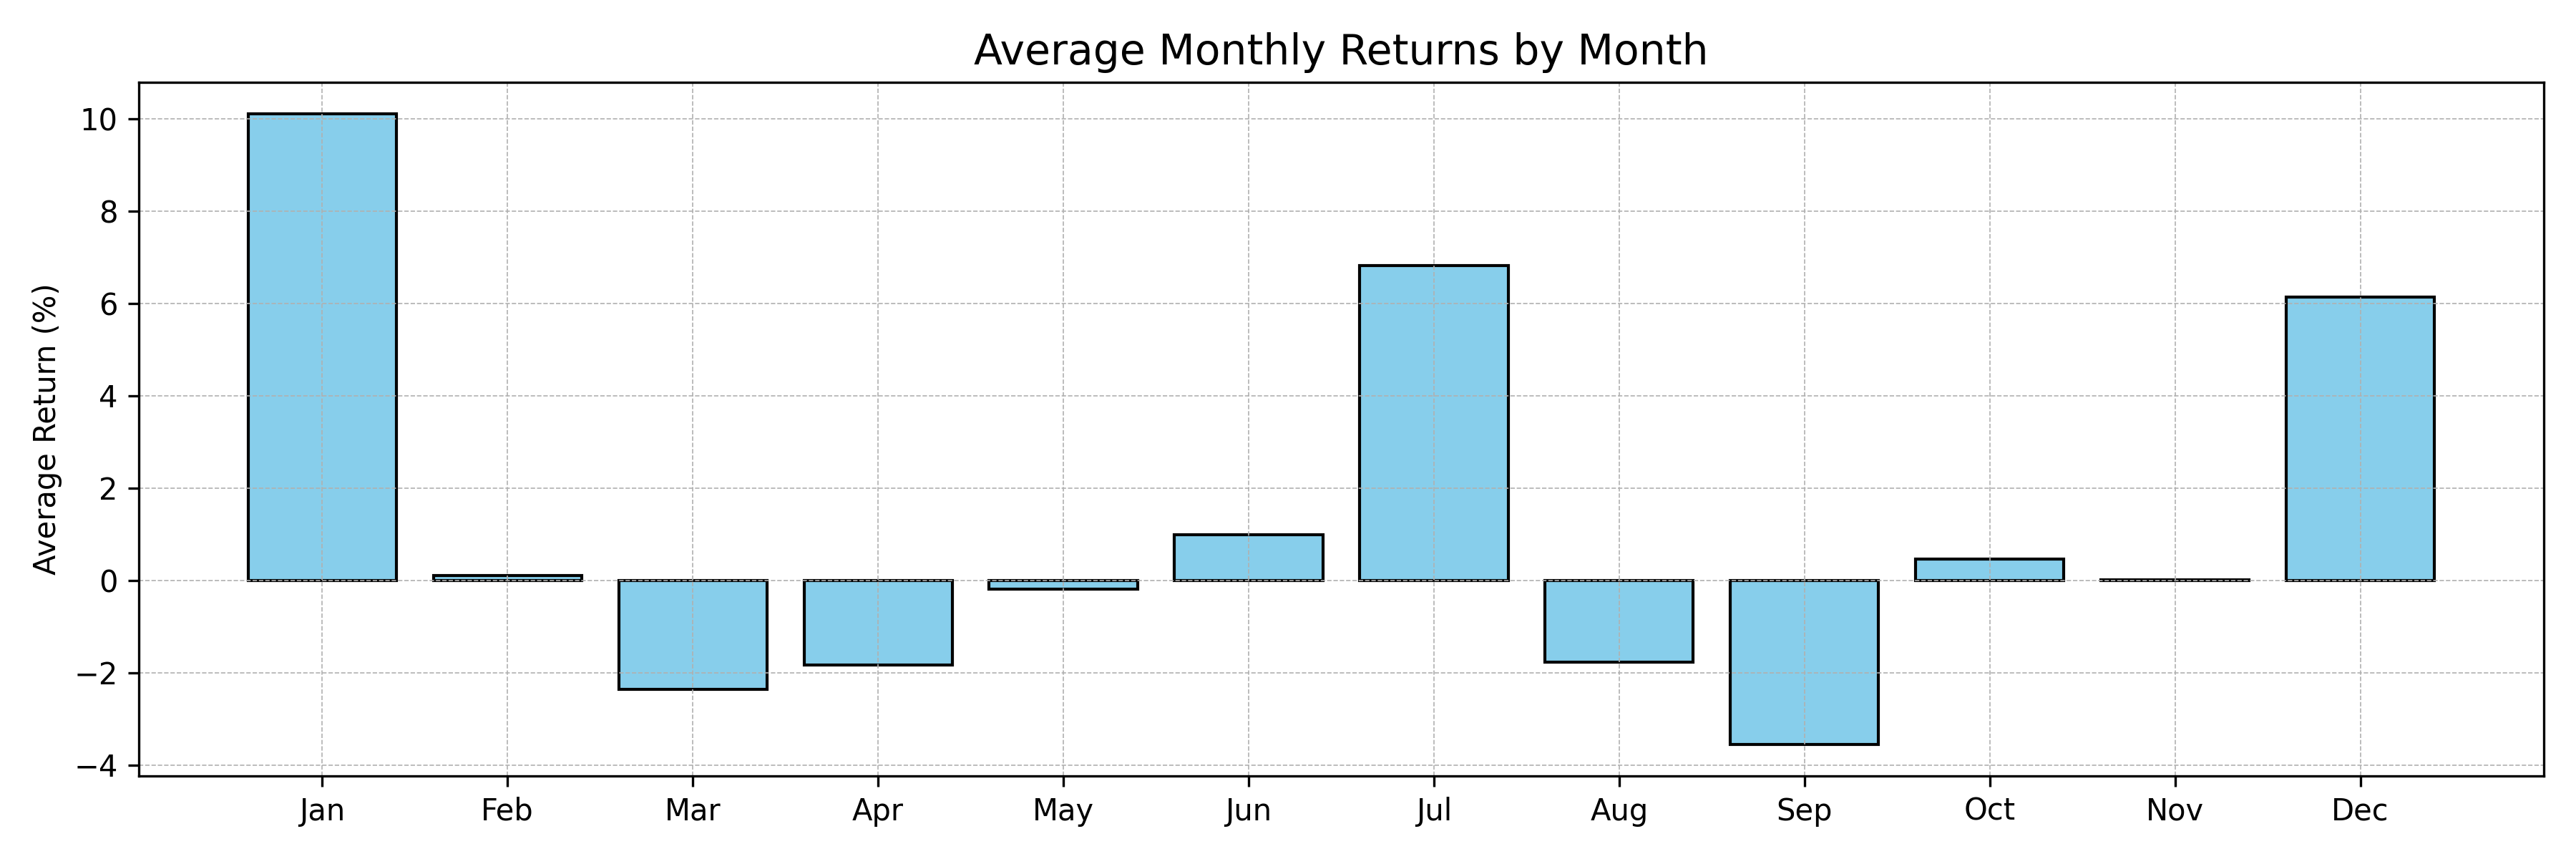
\includegraphics[width=0.7\textwidth]{decomposition_outputs/NONLIFEINSU_avg_monthly_returns.png}
    \caption{Average Monthly Returns by Month -- NONLIFEINSU}
\end{figure}

\begin{table}[h!]
\centering
\caption{Average Monthly Returns -- NONLIFEINSU}
\begin{tabular}{l r}
\toprule
Month & Value (\%) \\
\midrule
Jan & 10.10 \\
Feb & 0.11 \\
Mar & -2.37 \\
Apr & -1.83 \\
May & -0.18 \\
Jun & 0.99 \\
Jul & 6.82 \\
Aug & -1.77 \\
Sep & -3.55 \\
Oct & 0.46 \\
Nov & 0.01 \\
Dec & 6.14 \\
\bottomrule
\end{tabular}
\end{table}

\begin{table}[h!]
\centering
\caption{Average Seasonality -- NONLIFEINSU}
\begin{tabular}{l r}
\toprule
Month & Value (\%) \\
\midrule
Jan & 5.82 \\
Feb & 1.26 \\
Mar & 0.23 \\
Apr & -7.53 \\
May & -0.48 \\
Jun & 2.43 \\
Jul & 3.06 \\
Aug & -2.94 \\
Sep & -4.85 \\
Oct & -0.95 \\
Nov & 0.16 \\
Dec & 2.27 \\
\bottomrule
\end{tabular}
\end{table}


\clearpage

\subsection{OTHERS}
\textbf{Mean Monthly Return:} 1.19\% \\
\textbf{Median Monthly Return:} 0.61\% \\
\textbf{Standard Deviation:} 2.85\% \\
\textbf{Best Month:} Jul (6.32\%) \\
\textbf{Worst Month:} Mar (-4.06\%) \\
\textbf{Seasonal Amplitude:} 10.38\% \\
\textbf{August Return:} 0.12\% \\

\begin{figure}[h!]
    \centering
    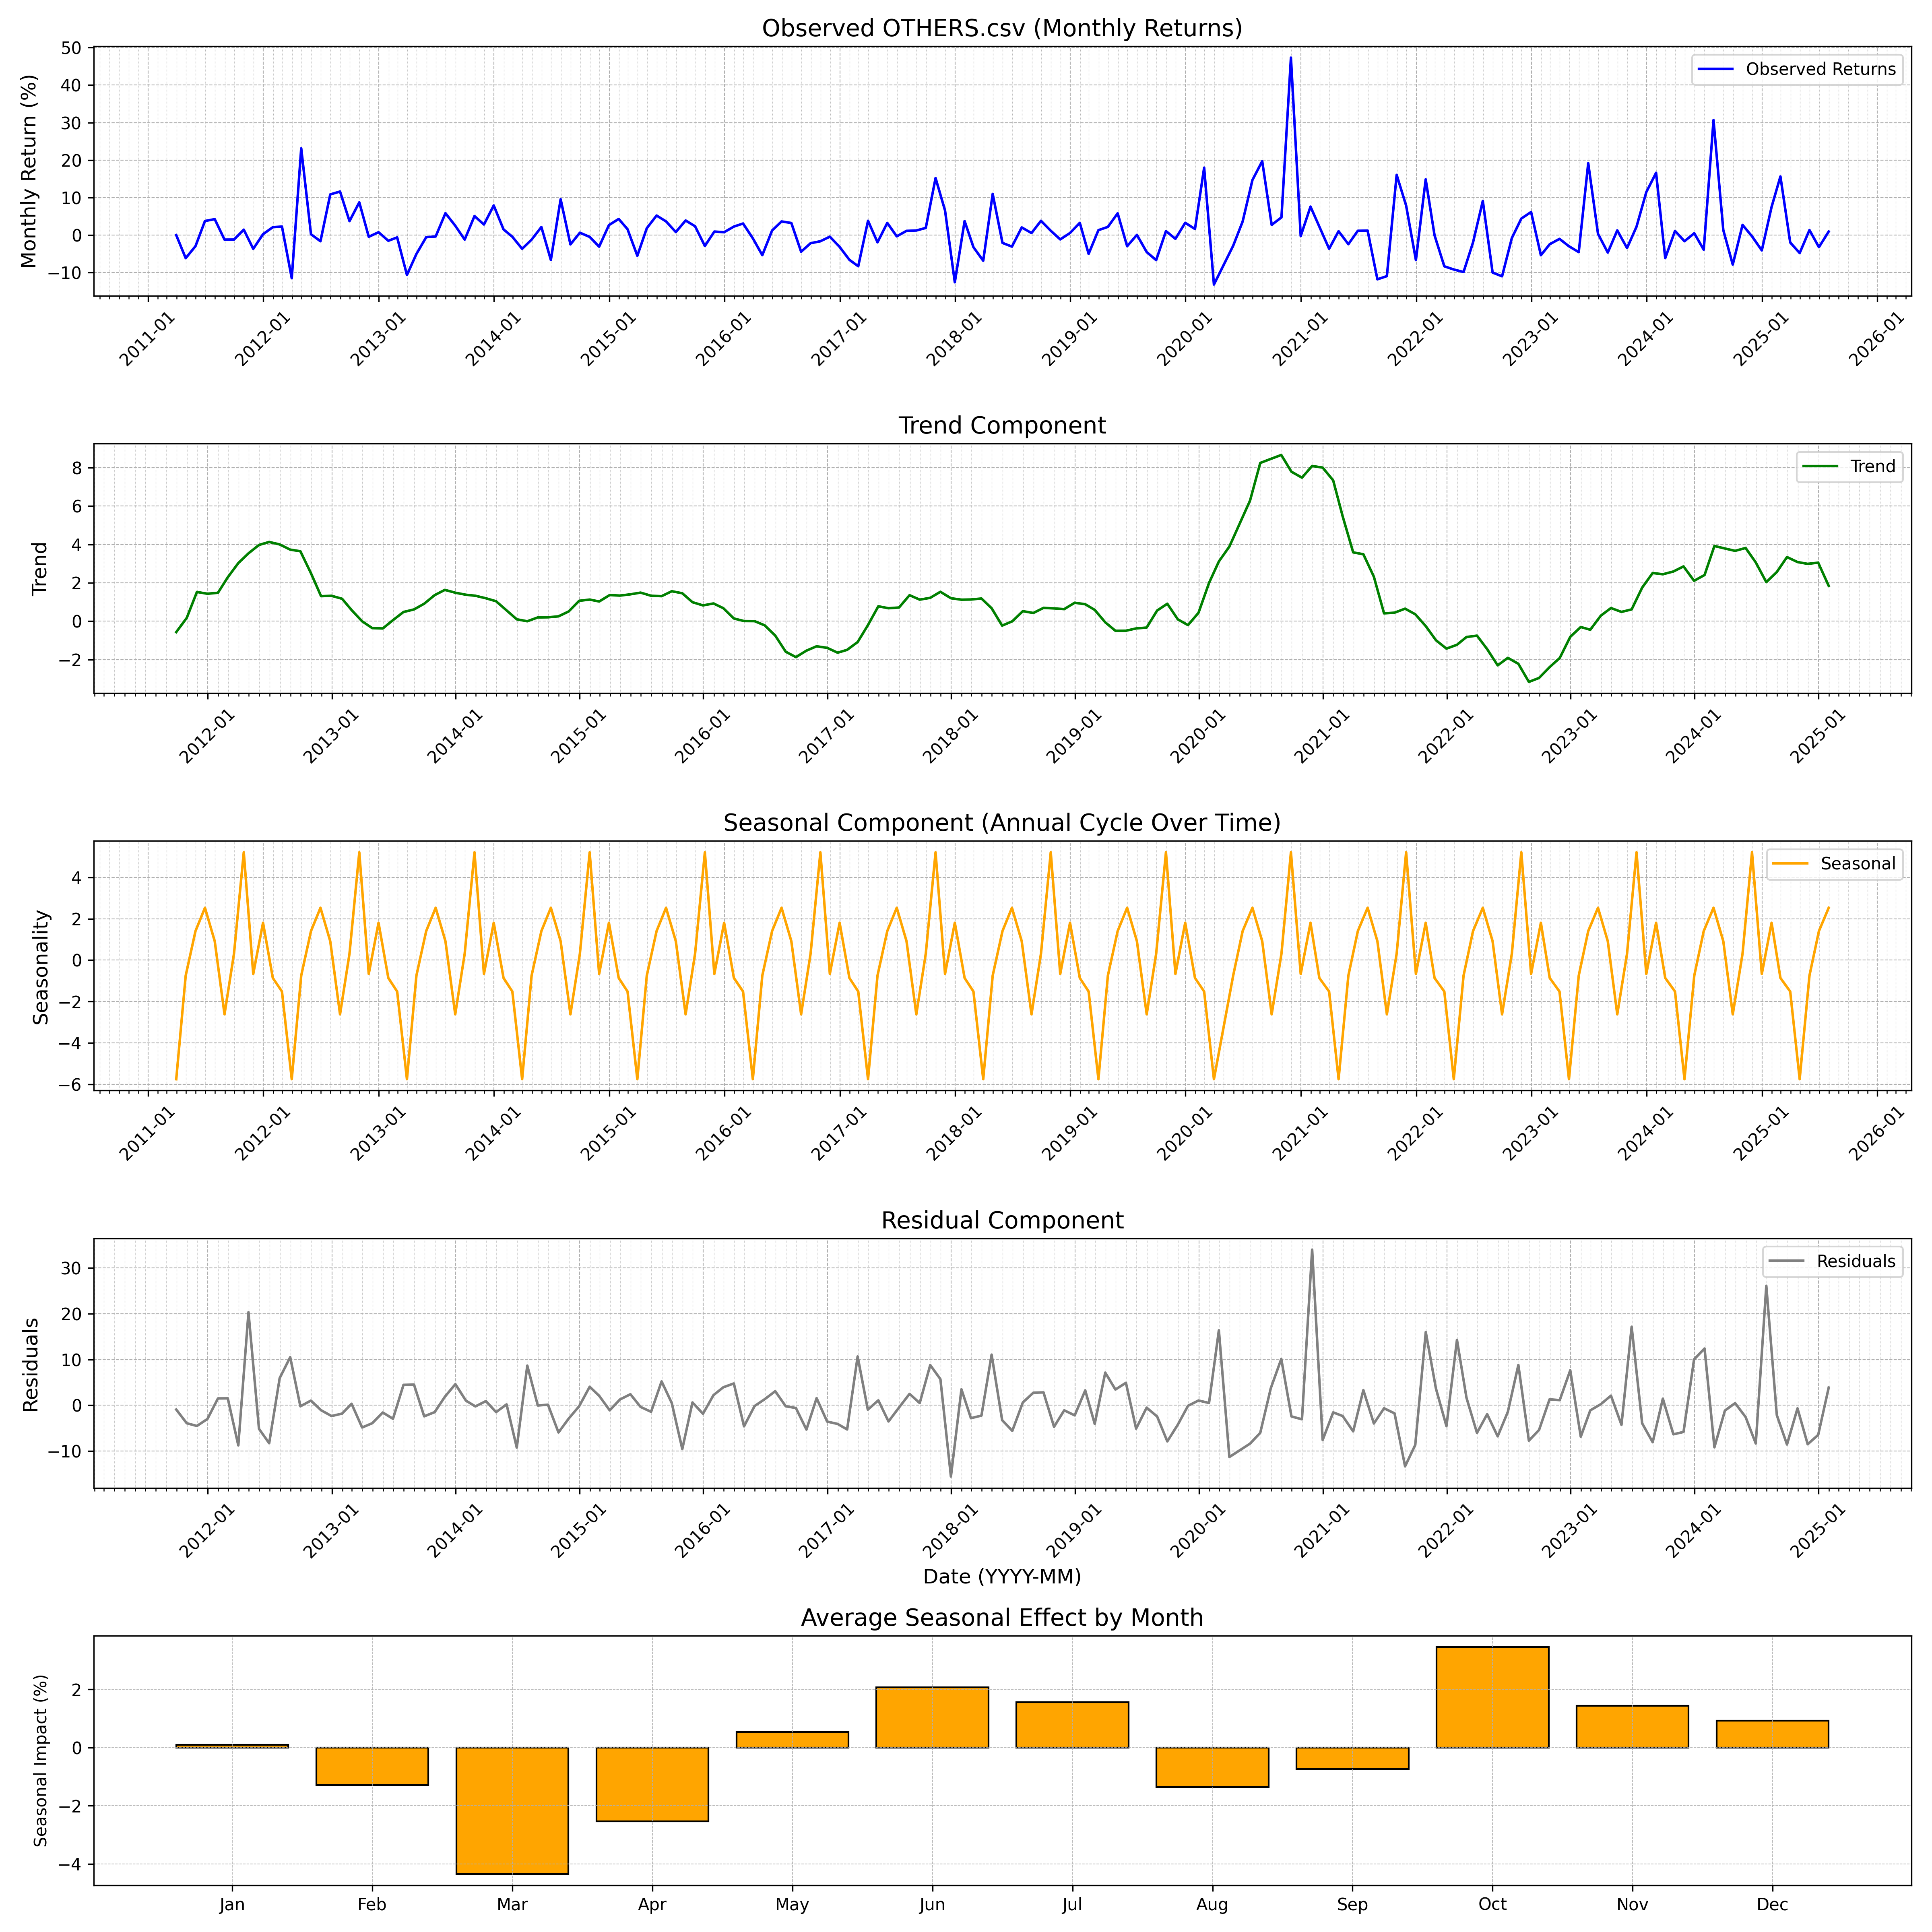
\includegraphics[width=0.9\textwidth]{decomposition_outputs/OTHERS_seasonal_decomposition.png}
    \caption{Seasonal Decomposition of OTHERS Index Monthly Returns}
\end{figure}

\begin{figure}[h!]
    \centering
    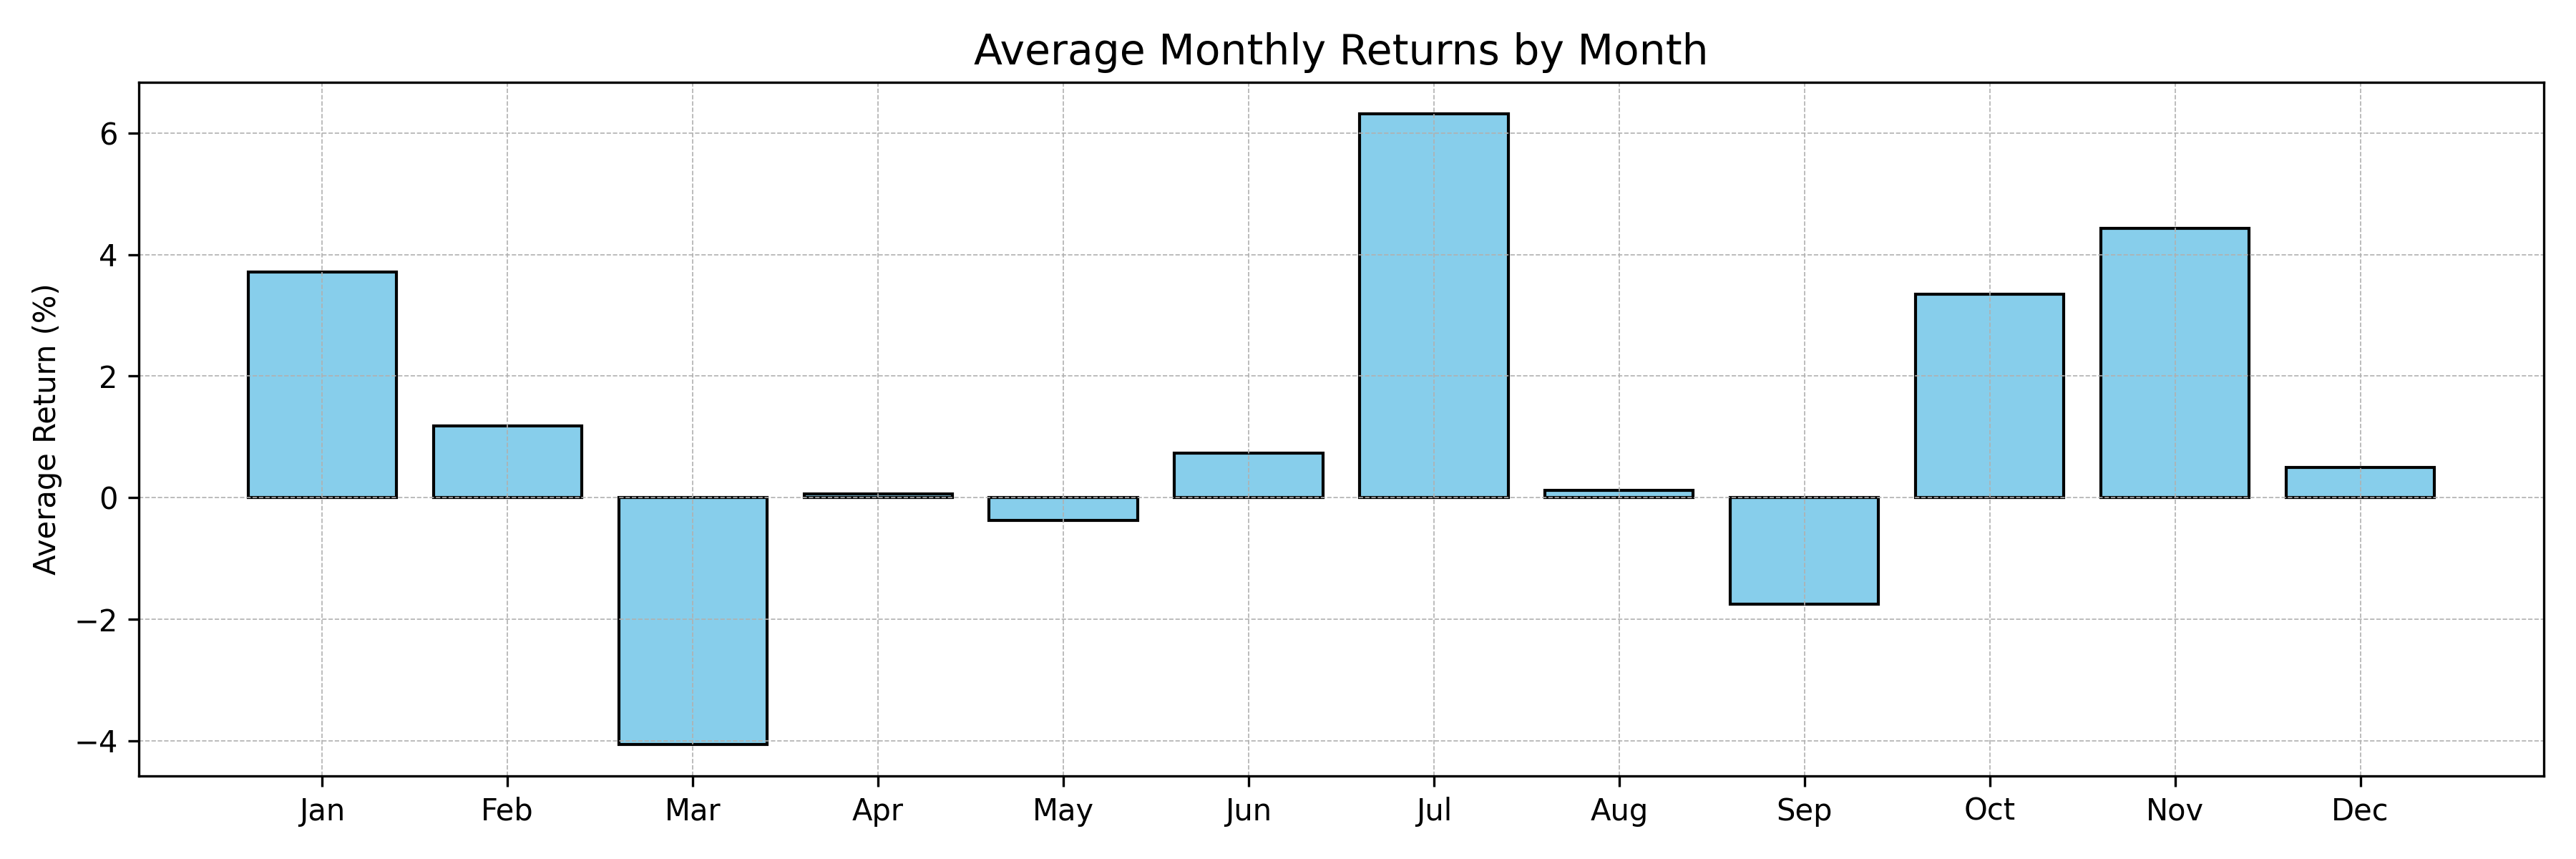
\includegraphics[width=0.7\textwidth]{decomposition_outputs/OTHERS_avg_monthly_returns.png}
    \caption{Average Monthly Returns by Month -- OTHERS}
\end{figure}

\begin{table}[h!]
\centering
\caption{Average Monthly Returns -- OTHERS}
\begin{tabular}{l r}
\toprule
Month & Value (\%) \\
\midrule
Jan & 3.71 \\
Feb & 1.19 \\
Mar & -4.06 \\
Apr & 0.07 \\
May & -0.37 \\
Jun & 0.73 \\
Jul & 6.32 \\
Aug & 0.12 \\
Sep & -1.76 \\
Oct & 3.35 \\
Nov & 4.43 \\
Dec & 0.50 \\
\bottomrule
\end{tabular}
\end{table}

\begin{table}[h!]
\centering
\caption{Average Seasonality -- OTHERS}
\begin{tabular}{l r}
\toprule
Month & Value (\%) \\
\midrule
Jan & 0.09 \\
Feb & -1.28 \\
Mar & -4.35 \\
Apr & -2.54 \\
May & 0.54 \\
Jun & 2.08 \\
Jul & 1.56 \\
Aug & -1.36 \\
Sep & -0.74 \\
Oct & 3.46 \\
Nov & 1.43 \\
Dec & 0.92 \\
\bottomrule
\end{tabular}
\end{table}


\clearpage

\subsection{TRADING}
\textbf{Mean Monthly Return:} 3.13\% \\
\textbf{Median Monthly Return:} 1.25\% \\
\textbf{Standard Deviation:} 5.71\% \\
\textbf{Best Month:} Nov (19.35\%) \\
\textbf{Worst Month:} Apr (-2.15\%) \\
\textbf{Seasonal Amplitude:} 21.50\% \\
\textbf{August Return:} 0.12\% \\

\begin{figure}[h!]
    \centering
    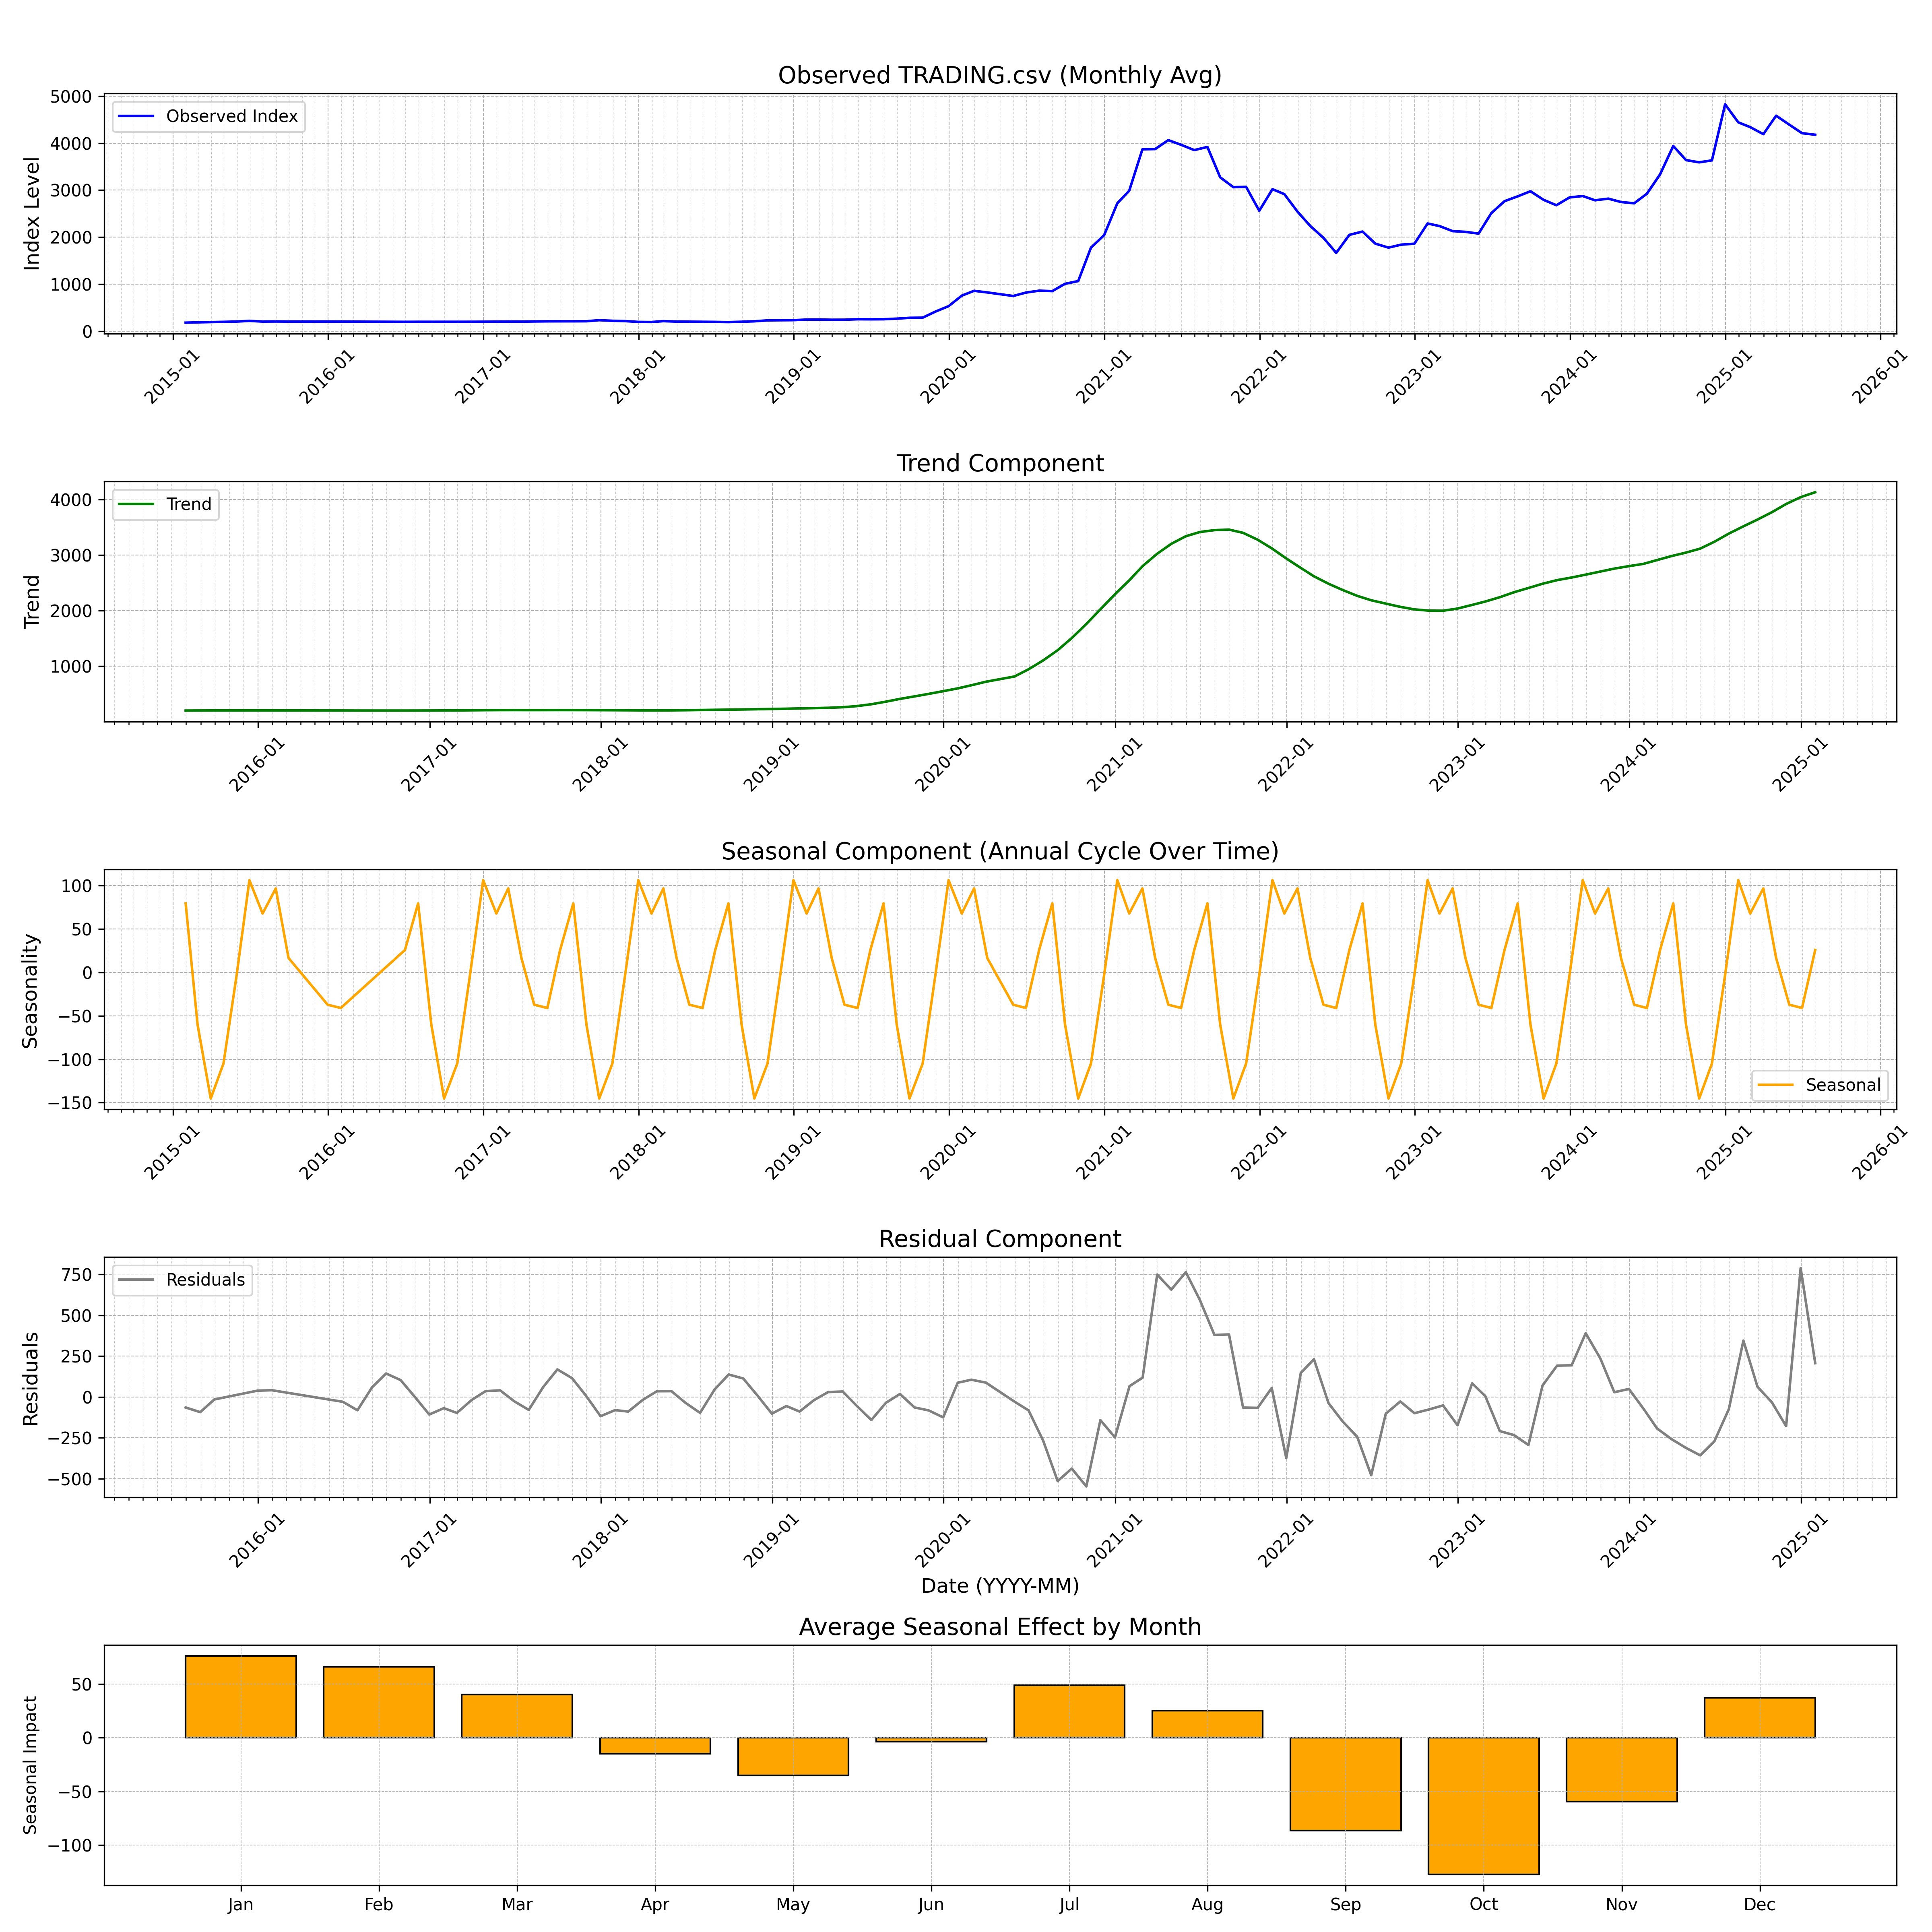
\includegraphics[width=0.9\textwidth]{decomposition_outputs/TRADING_seasonal_decomposition.png}
    \caption{Seasonal Decomposition of TRADING Index Monthly Returns}
\end{figure}

\begin{figure}[h!]
    \centering
    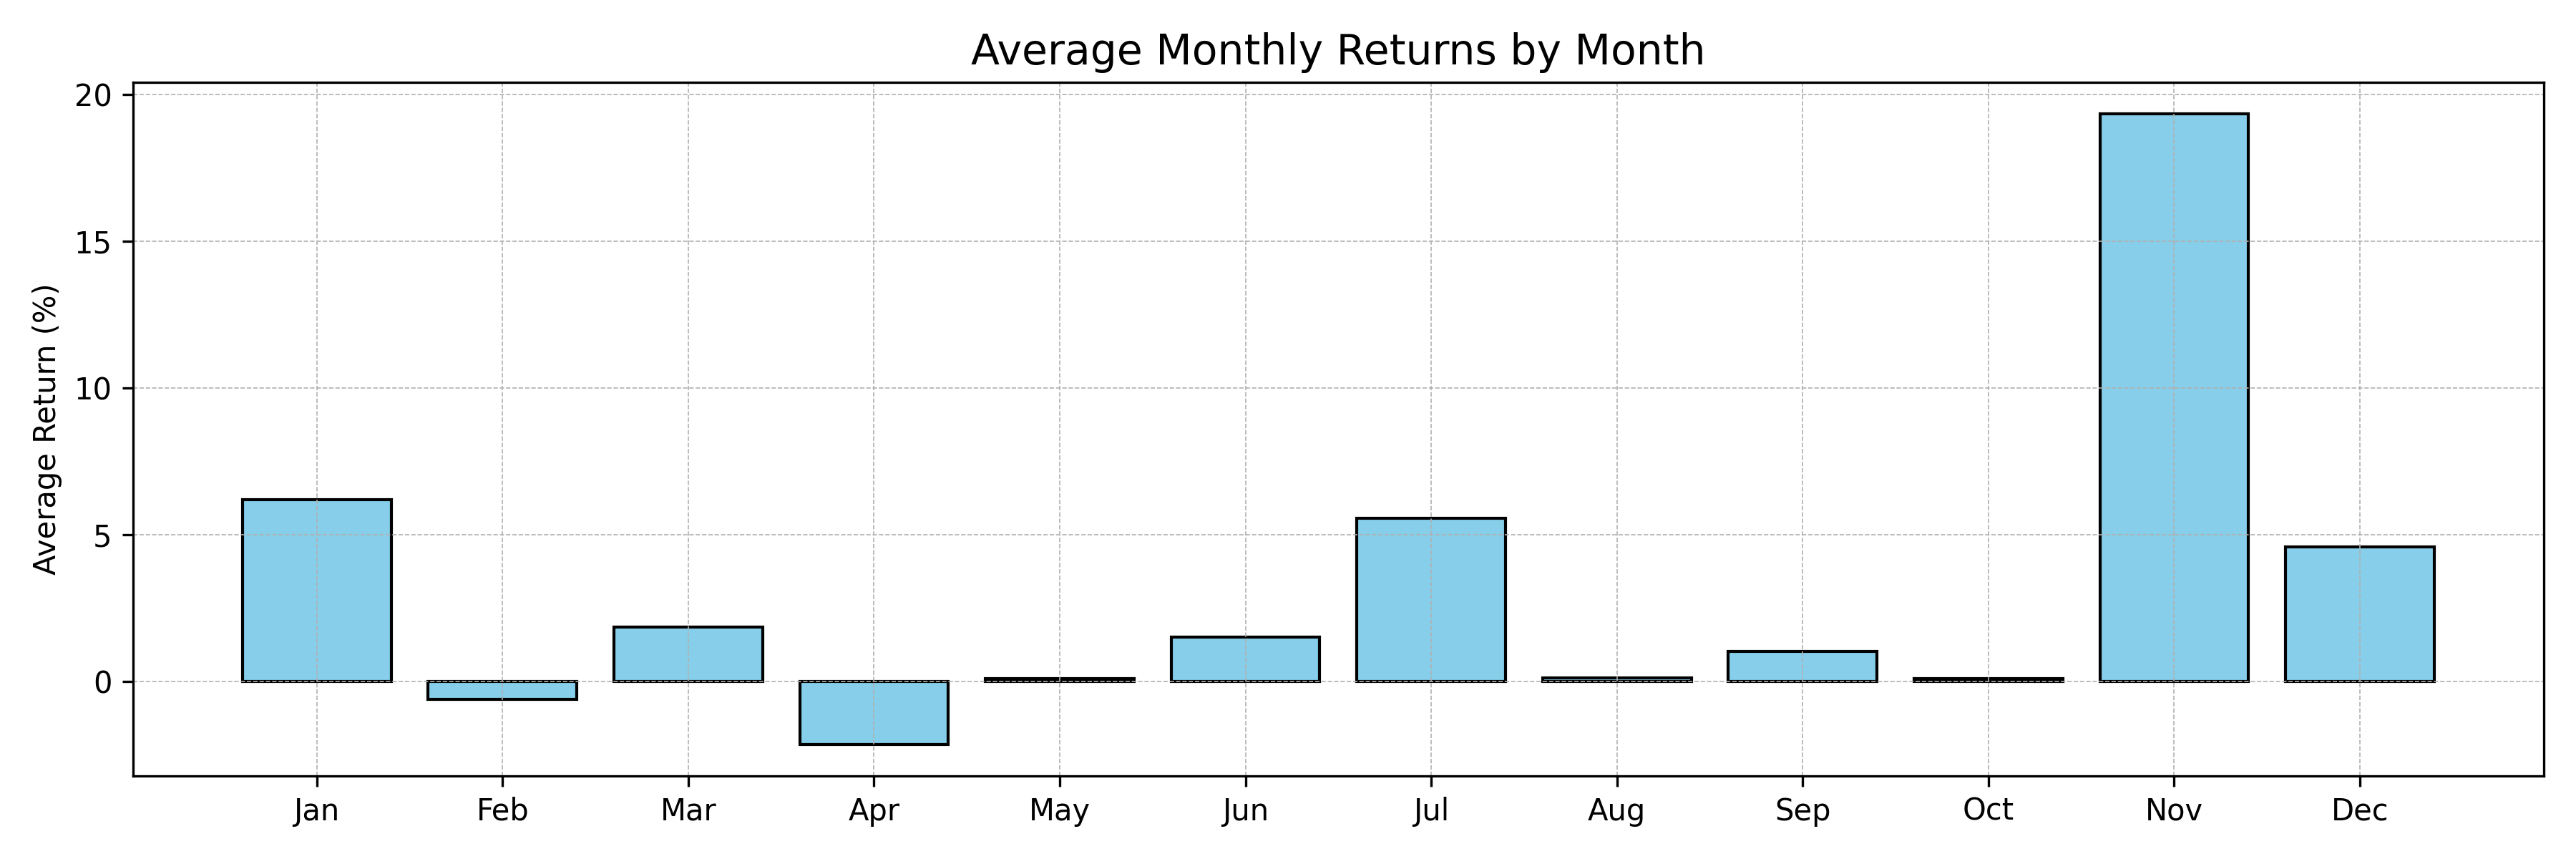
\includegraphics[width=0.7\textwidth]{decomposition_outputs/TRADING_avg_monthly_returns.png}
    \caption{Average Monthly Returns by Month -- TRADING}
\end{figure}

\begin{table}[h!]
\centering
\caption{Average Monthly Returns -- TRADING}
\begin{tabular}{l r}
\toprule
Month & Value (\%) \\
\midrule
Jan & 6.19 \\
Feb & -0.61 \\
Mar & 1.84 \\
Apr & -2.15 \\
May & 0.10 \\
Jun & 1.50 \\
Jul & 5.56 \\
Aug & 0.12 \\
Sep & 1.01 \\
Oct & 0.08 \\
Nov & 19.35 \\
Dec & 4.58 \\
\bottomrule
\end{tabular}
\end{table}

\begin{table}[h!]
\centering
\caption{Average Seasonality -- TRADING}
\begin{tabular}{l r}
\toprule
Month & Value (\%) \\
\midrule
Jan & 1.46 \\
Feb & -0.86 \\
Mar & -2.64 \\
Apr & -4.48 \\
May & -1.98 \\
Jun & 1.08 \\
Jul & 0.15 \\
Aug & -3.70 \\
Sep & -2.53 \\
Oct & 4.10 \\
Nov & 6.30 \\
Dec & 3.42 \\
\bottomrule
\end{tabular}
\end{table}


\clearpage

\section{Cross-Sector Statistical Summary}
\begin{table}[h!]
\centering
\caption{Summary Statistics Across Sectors}
\begin{tabular}{lcccccc}
\toprule
Sector & Mean & Std Dev & Best Month & Worst Month & Amplitude & August Ret \\
\midrule}
BANKING & 1.16\% & 3.24\% & Jul (9.30\%) & Mar (-2.16\%) & 11.46\% & -1.77\% \\
DEVBANK & 2.16\% & 3.31\% & Jul (9.92\%) & Sep (-1.75\%) & 11.67\% & -0.16\% \\
FINANCE & 1.48\% & 3.49\% & Jul (10.05\%) & Sep (-2.78\%) & 12.83\% & -1.93\% \\
HOTELS & 1.76\% & 2.75\% & Jul (6.40\%) & Aug (-2.52\%) & 8.92\% & -2.52\% \\
HYDROPOWER & 1.47\% & 2.93\% & Jan (6.78\%) & Aug (-3.06\%) & 9.84\% & -3.06\% \\
INVESTMENT & 0.39\% & 5.74\% & Jul (11.63\%) & Sep (-9.31\%) & 20.94\% & -5.92\% \\
LIFEINSU & 1.23\% & 4.43\% & Dec (9.06\%) & Sep (-3.70\%) & 12.76\% & -3.17\% \\
MANUFACTURE & 1.71\% & 2.52\% & Jul (5.72\%) & Mar (-2.69\%) & 8.41\% & 0.49\% \\
MICROFINANCE & 1.75\% & 4.80\% & Jan (11.78\%) & Mar (-3.46\%) & 15.24\% & -3.46\% \\
NONLIFEINSU & 1.24\% & 4.20\% & Jan (10.10\%) & Sep (-3.55\%) & 13.65\% & -1.77\% \\
OTHERS & 1.19\% & 2.85\% & Jul (6.32\%) & Mar (-4.06\%) & 10.38\% & 0.12\% \\
TRADING & 3.13\% & 5.71\% & Nov (19.35\%) & Apr (-2.15\%) & 21.50\% & 0.12\% \\
\bottomrule
\end{tabular}
\end{table}

\section{Interpretation and Investment Recommendations}
\subsection{Interpretation}
The analysis reveals robust and persistent seasonal patterns across NEPSE subindices. July is the most favorable month for returns, while August and September are consistently weak. The seasonal amplitude is highest in Investment, Insurance, and Microfinance sectors, indicating strong cyclical effects. Trend components are generally positive, supporting long-term sector growth, but are interrupted by cyclical corrections.

\subsection{Investment Recommendations}
\begin{itemize}
    \item \textbf{Tactical Allocation:} Overweight sectors in July and November (for Trading), underweight in August–September.
    \item \textbf{Risk Management:} Use volatility and drawdown statistics to size positions and set stop-losses.
    \item \textbf{Diversification:} Blend high-seasonality sectors (e.g., Investment, Microfinance) with more stable ones (e.g., Banking, Manufacture) to optimize risk-adjusted returns.
    \item \textbf{Further Research:} Investigate macroeconomic, regulatory, and behavioral drivers of observed seasonality.
    \item \textbf{Systematic Strategies:} Consider calendar-based rotation strategies, increasing exposure before July and reducing after, especially in sectors with high seasonal amplitude.
\end{itemize}

\section{Appendix}
All decomposition plots, tables, and code are available in the \texttt{decomposition\_outputs} directory.

\end{document}
